%By Douglas Bish
%The text is licensed under the
%\href{http://creativecommons.org/licenses/by-sa/4.0/}{Creative Commons
%Attribution-ShareAlike 4.0 International License}.
%
%This file has been modified by Robert Hildebrand 2020.  
%CC BY SA 4.0 licence still applies.


\documentclass[11pt,myequations,myarticle]{article}
\usepackage[top=1.0in, bottom=1.0in, left=1.0in, right=1.0in]{geometry}
\usepackage{latexsym}
\usepackage[pdftex]{graphicx}
\usepackage{amsmath}
\usepackage{amsfonts}
\usepackage{longtable}
\usepackage{color}   
\usepackage{colortbl}
\usepackage{hyperref}
\usepackage{tikz}
\usetikzlibrary{arrows, positioning, automata, patterns}
\usepackage{pgfplots} 
\usepackage{comment} %\begin{comment} \end{comment}
\hypersetup{
    colorlinks=true, % set to true if you want colored links
    linktoc=all,     % set to all if you want both sections and subsections linked
    linkcolor=blue,  % choose some color if you want links to stand out
}
\usepackage{titlesec}

\titleformat*{\section}{\LARGE\bfseries}
\titleformat*{\subsection}{\Large\bfseries}
\titleformat*{\subsubsection}{\Large\bfseries}


\usepackage{fancyhdr}
\pagestyle{fancy}
\fancyhf{}
%\fancyhead[RE]{\leftmark}
%\fancyhead[LO]{\rightmark}
\fancyfoot[C]{\thepage}
\fancyfoot[R]{\hyperlink {toc}{$\uparrow$}}
\fancypagestyle{plain}{%  the preset of fancyhdr 
    \fancyhf{} % clear all header and footer fields
    \fancyfoot[C]{\textbf{\thepage}} % except the center
    \renewcommand{\headrulewidth}{0pt}
    \renewcommand{\footrulewidth}{0pt}}

% Base colors: red, green, blue, cyan, magenta, yellow, black, gray, darkgray, lightgray, brown, lime, olive, orange, pink, purple, teal, violet and white. Mix colors: blue!50!cyan
% https://en.wikibooks.org/wiki/LaTeX/PGF/TikZ#Color

% https://www.ams.org/open-math-notes/omn-view-listing?listingId=110636
% https://sites.math.washington.edu/~burke/crs/407/notes/index.html

\def\sspace{ \renewcommand{\baselinestretch}{1.0}\small\normalsize}
\setlength\parindent{0pt} %\noindent for entire document

\cellcolor{red}

%\newcommand{\cr}[1]{\mathbf{#1}} % change to \mathbb

\newcommand{\rc}{\cellcolor{red}} % change cell color red in table
\newcommand{\hi}{\cellcolor{red}} % change cell color red in table

\newtheorem{example}{Example}%[section]
\newtheorem{ICE}{ICE}%[section]
\newtheorem{problem}{Problem}%[section]
\newtheorem{solution}{Solution}%[section]

\setcounter{tocdepth}{4}
\setcounter{secnumdepth}{4}







\begin{document} \pagenumbering{arabic} \setcounter{page}{0} \sspace
\begin{center}{\LARGE Optimization} \end{center} \Large
\tableofcontents


%\vspace{10mm} \fbox{\begin{minipage}{28em} \end{minipage}}


\newpage \section{Introduction to Optimization}
%By Douglas Bish
%The text is licensed under the
%\href{http://creativecommons.org/licenses/by-sa/4.0/}{Creative Commons
%Attribution-ShareAlike 4.0 International License}.
%
%This file has been modified by Robert Hildebrand 2020.  
%CC BY SA 4.0 licence still applies.


Optimization (i.e., Mathematical Programming) seeks to select, from a set of alternative solutions (decisions), a solution that is ``best" for a given performance criteria (i.e., maximize or minimizes the criteria). The following is a general optimization problem: 
$$ \text{max} \{f(\mathbf{x},\mathbf{y}): A(\mathbf{x)} + G(\mathbf{y}) \le \mathbf{b}_1, H(\mathbf{x)} + W(\mathbf{y}) =  \mathbf{b}_2, \mathbf{x} \in \mathcal{Z^+}, \mathbf{y} \in \mathcal{R^+}\},$$ 

where $\mathbf{x}$ and $\mathbf{y}$ are vectors of decision variables, $f(\mathbf{x},\mathbf{y})$ is the {\it objective function}, which defines the ``best'' solution (in this case the optimization problem seeks to maximize the objective function), and $A(\mathbf{x)} + G(\mathbf{y}) \le \mathbf{b}_1$, $H(\mathbf{x)} + W(\mathbf{y}) = \mathbf{b}_2$, $\mathbf{x} \in \mathcal{Z^+}$, and $\mathbf{y} \in \mathcal{R^+}$ are the {\it constraints} that define the set of possible solutions.


\bigskip Depending on the nature of the objective function, the constraints, and the input parameters, we can make some broad classifications of optimization problems, as follows:

\bigskip \underline{\bf Linear Optimization:} Linear optimization, i.e., a linear program (LP), has a linear objective function subject to a set of linear constraints and continuous decision variables.\\

 {\bf Definition:} A function $f(x_1,x_2,\cdots,x_n)$ is linear if, and only if, we have $f(x_1,x_2,\cdots,x_n) = c_1x_1 + c_2x_2 + \cdots + c_nx_n$, where the  $c_1,c_2,\cdots,c_n$ coefficients are constants.  \\

An LP has the following general form:
$$ \text{max} \{\mathbf{cx}: \mathbf{A}\mathbf{x} = \mathbf{b},  x \in \mathcal{R}\},$$ where $\mathbf{x}$ is a vector of decision variables, and the vectors $\mathbf{c}$ and $\mathbf{b}$, as well as the matrix $\mathbf{A}$, are constant problem parameters.

\bigskip \underline{\bf Nonlinear Optimization:} Nonlinear optimization, i.e., a nonlinear program, is similar to an LP, but objective function and/or the constraints are nonlinear. \\

\underline{\bf Integer Optimization:} Integer optimization, , i.e., an integer program (IP), is much like an LP, but some) variables restricted to take only integer values. \\
 
% Add others, ...
% Dynamic Program - Optimize a multi-stage problem, which is often recursive in nature.
% Stochastic Program - Optimize a problem where some of the input data is stochastic.
% Network Optimization - Optimize problems with special network structures.



\bigskip To use optimization, first you must formulate your model, based on the system of interest and any simplifications required (i.e., assumptions).  Formulating the model is not enough, we are also interested in solving the problem, and in a reasonable amount of time (however that is determined). To solve these problems, algorithms are developed.  An algorithms is a step-by-step process for finding a solution.  We can broadly define different types of algorithms as follows:
\begin{itemize}
\item Optimal algorithms - processes that solve the model to optimality (and proves optimality).
\item Near-optimal algorithms with bounds (heuristics), processes that do not guarantee optimality, but provides ``good" solutions with known bounds.
\item Other heuristic algorithms, processes that provide a ``good" solution, but bounds are not provided, or are not that useful.
\end{itemize}

Algorithms can also be categorized based on performance, for instance, usually a {\it polynomial time algorithm} is better than an {\it exponential time algorithm}.

\bigskip The class will almost exclusively focus on Linear Programs (LP) because: 1) LP are useful for many problems; 2) LPs are, relatively, easy to solve; and most importantly 3) LP are an important foundation for further courses in optimization.

\subsection{Notation}

\begin{itemize}
\item We use bold text to indicate a matrix or vector, e.g., the matrix ${\bf A}$ or the vector ${\bf x}$.
\end{itemize}

\newpage \section{Linear Optimization}
In this section, we study on linear optimization problems, i.e., linear programs (LPs).

\subsection{Problem Formulation} %By Douglas Bish
%The text is licensed under the
%\href{http://creativecommons.org/licenses/by-sa/4.0/}{Creative Commons
%Attribution-ShareAlike 4.0 International License}.
%
%This file has been modified by Robert Hildebrand 2020.  
%CC BY SA 4.0 licence still applies.


Remember, for a linear program (LP), we want to maximize or minimize a linear {\bf objective function} of the continous decision variables, while considering linear constraints on the values of the decision variables.

%\bigskip {\bf Definition:} 
\begin{definition}{Linear Function}
A function $f(x_1,x_2,\cdots,x_n)$ is \emph{linear} if, and only if, we have $f(x_1,x_2,\cdots,x_n) = c_1x_1 + c_2x_2 + \cdots + c_nx_n$, where the  $c_1,c_2,\cdots,c_n$ coefficients are constants.  
\end{definition}

\bigskip  \underline{\bf A Generic Linear Program (LP)}

\medskip  \underline{Decision Variables:}\\
$x_i$ : continuous variables ($x_i \in \mathcal{R}$, i.e., a real number), $\forall i = 1,\cdots,3$.

\medskip \underline{Parameters (known input parameters):}\\
$c_i$ : cost coefficients $\forall i = 1,\cdots,3$ \\
$a_{ij}$ : constraint coefficients $\forall i = 1,\cdots,3,~ j = 1,\cdots,4$ \\
$b_j$ : right hand side coefficient for constraint $j$, $j = 1,\cdots,4$

\begin{align}
\mbox{Min~~} & z = c_1x_1 + c_2x_2 + c_3x_3  \label{eq:OF1}\\
\mbox{s.t.~~} & a_{11}x_1 + a_{12}x_2 + a_{13} x_3 \ge b_1 \label{eq:C1} \\
& a_{21}x_1 + a_{22}x_2 + a_{23} x_3 \le b_2 \label{eq:C2} \\
& a_{31}x_1 + a_{32}x_2 + a_{33} x_3 = b_3 \label{eq:C3}\\
& a_{41}x_1 + a_{42}x_2 + a_{43} x_3 \ge b_4 \label{eq:C4}\\
& x_1 \ge 0, x_2 \le 0, x_3~urs \label{eq:C5}.
\end{align}

Eq.~(\ref{eq:OF1}) is the objective function, (\ref{eq:C1})-(\ref{eq:C4}) are the functional constraints, while (\ref{eq:C5}) is the sign restrictions ({\it ur}s signifies that the variable is unrestricted). If we were to add any one of these following constraints $x_2 \in \{0, 1\}$ ($x_2$ is binary-valued) or $x_3 \in \mathcal{Z}$ ($x_3$ is integer-valued) we would have an Integer Program.  For the purposes of this class, an Integer Program (IP) is just an LP with added integer restrictions on (some) variables.

While, in general, solvers will take any form of the LP, there are some special forms we use in analysis:\\

\medskip \underline{\bf LP Standard Form}: The standard form has all constraints as equalities, and all variables as non-negative.  The generic LP is not in standard form, but any LP can be converted to standard form. \\

Since $x_2$ is non-positive and $x_3$ unrestricted, perform the following substitutions $x_2=-\hat{x}_2$ and $x_3 = x_3^+ -x_3^-$, where $\hat{x}_2$, $x_3^+$, $x_3^- \ge 0$.   Eqs.~(\ref{eq:C1}) and (\ref{eq:C4}) are in the form left-hand side (LHS) $\ge$ right-hand side (RHS), so to make an equality, subtract a non-negative slack variable from the LHS ($s_1$ and $s_4$).  Eq.~(\ref{eq:C2}) is in the form LHS $\le$ RHS, so add a non-negative slack variable to the LHS.
\begin{align*}
\mbox{Min~~} & z = c_1x_1 - c_2\hat{x}_2 + c_3 (x_3^+ -x_3^-)  \\
\mbox{s.t.~~} & a_{11}x_1 - a_{12}x_2 + a_{13} (x_3^+ -x_3^-) - s_1 = b_1 \\
& a_{21}x_1 - a_{22}\hat{x}_2 + a_{23} (x_3^+ -x_3^-) + s_2 = b_2 \\
&  a_{31}x_1 - a_{32}\hat{x}_2 + a_{33} (x_3^+ -x_3^-) = b_3 \\
& a_{41}x_1 - a_{42}\hat{x}_2 + a_{43} x_3 - s_4 = b_4 \\
& x_1, \hat{x}_2, x_3^+, x_3^-, s_1, s_2, s_4 \ge 0.
\end{align*}

\medskip \underline{\bf  LP Canonical Form}: For a minimization problem the canonical form of the LP has the LHS of each constraint greater than or equal to the the RHS, and a maximization the LHS less than or equal to the RHS, and non-negative variables.

Next we consider some formulation examples:

\bigskip  {\bf Production Problem:} You have 21 units of transparent aluminum alloy (TAA), LazWeld1, a joining robot leased for 23 hours, and CrumCut1, a cutting robot leased for 17 hours of aluminum cutting. You also have production code for a bookcase, desk, and cabinet, along with commitments to buy any of these you can produce for \$18,  \$16, and  \$10 apiece, respectively.  A bookcase requires 2 units of TAA, 3 hours of joining, and 1 hour of cutting, a desk requires 2 units of TAA, 2 hours of joining, and 2 hour of cutting, and a cabinet requires 1 unit of TAA, 2 hours of joining, and 1 hour of cutting. Formulate an LP to maximize your revenue given your current resources.

\medskip \underline{Decision variables:} \\
$x_i$ : number of units of product $i$ to produce, \\
$\forall i = \{bookcase,~desk,~cabinet\}$.
\begin{align*}
\max~& z = 18x_1 + 16x_2 + 10x_3 :  \\
& 2x_1 + 2x_2 + 1x_3 \le 21 & (TAA) \\
& 3x_1 + 2x_2 + 2x_3 \le 23 & (LazWeld1) \\
&  1x_1 + 2x_2 + 1x_3 \le 17 & (CrumCut1)  \\
& x_1, x_2, x_3 \ge 0.
\end{align*}





\bigskip {\bf Work Scheduling Problem:} You are the manager of LP Burger. The following table shows the minimum number of employees required to staff the restaurant on each day of the week. Each employees must work for five consecutive days. Formulate an LP to find the minimum number of employees required to staff the restaurant.

\begin{table}[h!] \begin{center} \begin{tabular} {|l|l|} 
\hline Day of Week & Workers Required   \\ \hline
\hline  1 = Monday & 6  \\
\hline  2 = Tuesday & 4  \\
\hline  3 = Wednesday & 5  \\
\hline  4 = Thursday & 4  \\
\hline  5 = Friday & 3  \\
\hline  6 = Saturday & 7  \\
\hline  7 = Sunday & 7  \\
\hline \end{tabular} \end{center} \end{table}

\underline{Decision variables:} \\
$x_i$ : the number of workers that start 5 consecutive days of work on day $i$, $ i = 1,\cdots,7$ \\

\begin{align*}
\mbox{Min~~ } & z = x_1 + x_2 + x_3 + x_4 + x_5 + x_6 + x_7  \\
\mbox{s.t.~~} & x_1 + x_4 + x_5 + x_6 + x_7 \ge 6 \\
& x_2 + x_5 + x_6 + x_7 + x_1 \ge 4 \\
& x_3 + x_6 + x_7 + x_1 + x_2 \ge 5 \\
& x_4 + x_7 + x_1 + x_2 + x_3 \ge 4 \\
& x_5 + x_1 + x_2 + x_3 + x_4 \ge 3 \\
& x_6 + x_2 + x_3 + x_4 + x_5 \ge 7 \\
& x_7 + x_3 + x_4 + x_5 + x_6 \ge 7 \\
& x_1, x_2, x_3, x_4, x_5, x_6, x_7 \ge 0.
\end{align*}

The solution is as follows:
\begin{table}[h!] \begin{center} \begin{tabular} {|l|l|}
\hline   LP Solution        & IP Solution \\
\hline  $z_{LP} = 7.333$    & $z_I = 8.0$ \\
\hline  $x_1 = 0$           & $x_1 = 0$ \\
\hline  $x_2 = 0.333$       & $x_2 = 0 $ \\
\hline  $x_3 = 1$           & $x_3 = 0$ \\
\hline  $x_4 = 2.333$       & $x_4 = 3$ \\
\hline  $x_5 = 0$           & $x_5 = 0 $ \\
\hline  $x_6 = 3.333$       & $x_6 = 4 $ \\
\hline  $x_7 = 0.333$       & $x_7 = 1 $ \\
\hline
\end{tabular} \end{center} \end{table}

\medskip  LP Burger has changed it's policy, and allows, at most, two part time workers, who work for two consecutive days in a week.  Formulate this problem.

\underline{Decision variables:} \\
$x_i$ : the number of workers that start 5 consecutive days of work on day $i$, $ i = 1,\cdots,7$ \\
$y_i$ : the number of workers that start 2 consecutive days of work on day $i$, $ i = 1,\cdots,7$.

\begin{align*}
\mbox{Min~~ } & z = 5(x_1 + x_2 + x_3 + x_4 + x_5 + x_6 + x_7) \\
& + 2(y_1 + y_2 + y_3 + y_4 + y_5 + y_6 + y_7) \nonumber \\
\mbox{s.t.~~} & x_1 + x_4 + x_5 + x_6 + x_7 + y_1 + y_7 \ge 6 \\
& x_2 + x_5 + x_6 + x_7 + x_1 + y_2 + y_1 \ge 4 \\
&           x_3 + x_6 + x_7 + x_1 + x_2 + y_3 + y_2 \ge 5 \\
&           x_4 + x_7 + x_1 + x_2 + x_3 + y_4 + y_3 \ge 4 \\
&           x_5 + x_1 + x_2 + x_3 + x_4 + y_5 + y_4 \ge 3 \\
&           x_6 + x_2 + x_3 + x_4 + x_5 + y_6 + y_5 \ge 7 \\
&           x_7 + x_3 + x_4 + x_5 + x_6 + y_7 + y_6 \ge 7 \\
&           y_1 + y_2 + y_3 + y_4 + y_5 + y_6 + y_7 \le 2 \\
&           x_i \ge 0, y_i \ge 0, \forall i = 1,\cdots,7.
\end{align*}

\bigskip  {\bf The Diet Problem:} In the future (as envisioned in a bad 70's science fiction film) all food is in tablet form, and there are four types, green, blue, yellow, and red. A balanced, futuristic diet requires, at least 20 units of Iron, 25 units of Vitamin B, 30 units of Vitamin C, and 15 units of Vitamin D. Formulate an LP that ensures a balanced diet at the minimum possible cost.

\begin{table}[h!] \begin{center} \begin{tabular} {|c|c|c|c|c|c|}
\hline Tablet  & Iron &  B &  C  &  D & Cost (\$) \\ \hline
\hline  green (1)  & 6    & 6  & 7          & 4        &  1.25 \\
\hline  blue (2)  & 4    & 5  & 4          & 9        &  1.05 \\
\hline  yellow (3) & 5    & 2  & 5          & 6        &  0.85 \\
\hline  red (4)   & 3    & 6  & 3          & 2        &  0.65 \\ \hline
\end{tabular} \end{center} \end{table}

Now we formulate the problem:

\smallskip  \underline{Decision variables:} \\
$x_i$ : number of tablet of type $i$ to include in the diet, $\forall i \in \{1,2,3,4\}$.
\begin{align*}
\mbox{Min~~ } & z = 1.25x_1 + 1.05x_2 + 0.85x_3 + 0.65x_4 \\
\mbox{s.t.~~} &  6x_1 + 4x_2 + 5x_3 + 3x_4 \ge 20  \\
& 6x_1 + 5x_2 + 2x_3 + 6x_4 \ge 25 \\
& 7x_1 + 4x_2 + 5x_3 + 3x_4 \ge 30 \\
& 4x_1 + 9x_2 + 6x_3 + 2x_4 \ge 15  \\
& x_1, x_2, x_3, x_4 \ge 0. 
\end{align*}

%The optimal diet costs \$5.35, and consists of 4.0625 green tablets and 0.3125 blue tablets.

\bigskip  {\bf The Next Diet Problem:} Progress is important, and our last problem had too many tablets, so we are going to produce a single, purple, 10 gram tablet for our futuristic diet requires, which are at least 20 units of Iron, 25 units of Vitamin B, 30 units of Vitamin C, and 15 units of Vitamin D, and 2000 calories. The tablet is made from blending 4 nutritious chemicals; the following table shows the units of our nutrients per, and cost of, grams of each chemical.
\begin{table}[h!] \begin{center} \begin{tabular} {|c|c|c|c|c|c|c|}
\hline Tablet  & Iron  &  B &  C &  D & Calories & Cost (\$) \\ \hline
\hline  Chem 1  & 6    & 6         & 7         & 4         &  1000    & 1.25 \\
\hline  Chem 2  & 4    & 5         & 4         & 9         &  250     & 1.05 \\
\hline  Chem 3  & 5    & 2         & 5         & 6         &  850     & 0.85 \\
\hline  Chem 4  & 3    & 6         & 3         & 2         &  750     & 0.65 \\
\hline
\end{tabular} \end{center} \end{table}
Formulate an LP that ensures a balanced diet at the minimum possible cost.

\smallskip \underline{Decision variables:} \\
$x_i$ : grams of chemical $i$ to include in the purple tablet, $\forall i = 1,2,3,4$.
\begin{align*}
\mbox{Min} & z = 1.25x_1 + 1.05x_2 + 0.85x_3 + 0.65x_4 \\
\mbox{s.t.~~} &  6x_1 + 4x_2 + 5x_3 + 3x_4 \ge 20 \\
& 6x_1 + 5x_2 + 2x_3 + 6x_4 \ge 25  \\
& 7x_1 + 4x_2 + 5x_3 + 3x_4 \ge 30  \\
& 4x_1 + 9x_2 + 6x_3 + 2x_4 \ge 15  \\
& 1000x_1 + 250x_2 + 850x_3 + 750x_4 \ge 2000 \\
& x_1 + x_2 + x_3 + x_4 = 10  \\
& x_1, x_2, x_3, x_4 \ge 0. 
\end{align*}

\bigskip {\bf The Assignment Problem:} Consider the assignment of $n$ teams to $n$ projects, where each team ranks the projects, where their favorite project is given a rank of $n$, their next favorite $n-1$, and their least favorite project is given a rank of 1.  The assignment problem is formulated as follows (we denote ranks using the $R$-parameter):

\smallskip \underline{Variables:} \\
$x_{ij}$ : 1 if project $i$ assigned to team $j$, else 0.
\begin{align*}
\mbox{Max~}   & z = \sum_{i=1}^{n}\sum_{j=1}^{n} R_{ij} x_{ij}  \\
\mbox{s.t.~}& \sum_{i=1}^{n} x_{ij} = 1,~~ \forall j = 1,\cdots,n  \\
& \sum_{j=1}^{n} x_{ij} = 1,~~ \forall i = 1,\cdots,n  \\
& x_{ij} \ge 0,~~ \forall i = 1,\cdots,n, j = 1,\cdots,n. 
\end{align*}
The assignment problem has an integrality property, such that if we remove the binary restriction on the $x$ variables (now just non-negative, i.e., $x_{ij} \ge 0$) then we still get binary assignments, despite the fact that it is now an LP.  This property is very interesting and useful. Of course, the objective function might not quite what we want, we might be interested ensuring that the team with the worst assignment is as good as possible (a fairness criteria). One way of doing this is to modify the assignment problem using a max-min objective:

\medskip {\bf Max-min Assignment-like Formulation} \\
\begin{eqnarray}
& Max  & z  \nonumber \\
& s.t. & \sum_{i=1}^{n} x_{ij} = 1,~~ \forall j = 1,\cdots,n \nonumber \\
&      & \sum_{j=1}^{n} x_{ij} = 1,~~ \forall i = 1,\cdots,n \nonumber \\
&      & x_{ij} \ge 0,~~ \forall i = 1,\cdots,n, J = 1,\cdots,n \nonumber \\
&      & z \le \sum_{i=1}^{n} R_{ij} x_{ij},~~ \forall j = 1,\cdots,n. \nonumber
\end{eqnarray}
Does this formulation have the integrality property (it is not an assignment problem)?  Consider a very simple example where two teams are to be assigned to two projects and the teams give the projects the following rankings:
\begin{table}[h!] \begin{center} \begin{tabular} {|c||c|c|}
\hline           & Project~1 & Project~2 \\ \hline \hline
\hline Team 1    & 2  & 1  \\
\hline Team 2    & 2  & 1 \\ \hline
\end{tabular} \end{center} \end{table}
Both teams prefer Project 2.  For both problems, if we remove the binary restriction on the
$x$-variable, they can take values between (and including) zero and one. For the assignment problem the optimal solution will have $z=3$, and fractional $x$-values will not improve $z$. For the max-min assignment problem this is not the case, the optimal solution will have $z=1.5$, which occurs when each team is assigned half of each project (i.e., for Team 1 we have $x_{11} = 0.5$ and $x_{21} = 0.5$).


\newpage \bigskip  {\bf Linear Data Models:} Consider a data set that consists of $n$ data points $(x_i,y_i)$.  We want to fit the best line to this data, such that given an $x$-value, we can predict the associated $y$-value.  Thus, the form is $y_ i = \alpha x_i + \beta$ and we want to choose the $\alpha$ and $\beta$ values such that we minimize the error for our $n$ data points.

\smallskip  \underline{\bf Variables:}\\
$e_i$ : error for data point $i$, $i = 1,\cdots,n$. \\
$\alpha$ : slope of fitted line. \\
$\beta$ : intercept of fitted line.
\begin{eqnarray}
& Min   & \sum_{i=1}^n |e_i|  \nonumber \\
& s.t.  & \alpha x_i + \beta - y_i = e_i,~~ i=1,\cdots,n \nonumber \\
&       & e_i, \alpha, \beta ~ urs \nonumber.
\end{eqnarray}

Of course, absolute values are not linear function, so we can linearize as follows:

\smallskip  \underline{\bf Decision variables:}\\
$e_i^+$ : positive error for data point $i$, $i = 1,\cdots,n$. \\
$e_i^-$ : negative error for data point $i$, $i = 1,\cdots,n$. \\
$\alpha$ : slope of fitted line. \\
$\beta$ : intercept of fitted line.
\begin{eqnarray}
& Min   & \sum_{i=1}^n e_i^+ +e_i^- \nonumber \\
& s.t.  & \alpha x_i + \beta - y_i = e_i^+-e_i^-,~~ i=1,\cdots,n \nonumber \\
&       & e_i^+, e_i^- \ge 0, \alpha, \beta ~ urs \nonumber.
\end{eqnarray}
 
\bigskip {\bf Two-Person Zero-Sum Games:} Consider a game with two players, $\mathcal{A}$ and $\mathcal{B}$. In each round of the game, $\mathcal{A}$ chooses one out of $m$ possible actions, while $\mathcal{B}$ chooses one out of $n$ actions.  If $\mathcal{A}$ takes action $j$ while $\mathcal{B}$ takes action $i$, then $c_{ij}$ is the payoff for $\mathcal{A}$ , if $c_{ij} > 0$, $\mathcal{A}$ ``wins" $c_{ij}$ (and $\mathcal{B}$ losses that amount), and if $c_{ij} < 0$ if $\mathcal{B}$ ``wins" $-c_{ij}$ (and $\mathcal{A}$ losses that amount).  This is a two-person zero-sum game.

\smallskip Rock, Paper, Scissors is a two-person zero-sum game, with the following payoff matrix.
\begin{center} \begin{tabular}{c|c|c|c|c|}
\multicolumn{5}{ c }{~~~~$\mathcal{A}$} \\ \cline{2-5}
              &         & {\bf R} & {\bf P} & {\bf S} \\ \cline{2-5}
              & {\bf R} & 0       & 1       & -1      \\ \cline{2-5}
$\mathcal{B}$ & {\bf P} & -1      & 0       & 1       \\ \cline{2-5}
              & {\bf S} & 1       & -1      & 0       \\ \cline{2-5}
\end{tabular} \end{center}

\smallskip  We can have a similar game, but with a different payoff matrix, as follows:
\begin{center} \begin{tabular}{c|c|c|c|c|}
\multicolumn{5}{ c }{~~~~$\mathcal{A}$} \\ \cline{2-5}
              &         & {\bf R} & {\bf P} & {\bf S} \\ \cline{2-5}
              & {\bf R} & 4       & -1      & -1 \\ \cline{2-5}
$\mathcal{B}$ & {\bf P} & -2      & 4       & -2 \\ \cline{2-5}
              & {\bf S} & -3      & -3      & 4 \\ \cline{2-5}
\end{tabular} \end{center}

\medskip What is the optimal strategy for $\mathcal{A}$ (for either game)? We define $x_j$ as the probability that $\mathcal{A}$ takes action $j$ (related to the columns).  Then the payoff for $\mathcal{A}$, if $\mathcal{B}$ takes action $i$ is $\sum_{j=1}^m c_{ij}x_{j}$. Of course, $\mathcal{A}$ does not know what action $\mathcal{B}$ will take, so let's find a strategy that maximizes the minimum expected winnings of $\mathcal{A}$ given any random strategy of $\mathcal{B}$, which we can formulate as follows:
\begin{eqnarray}
& Max  & (min_{i=1,\cdots,n} \sum_{j=1}^m  c_{ij}x_i) \nonumber \\
& s.t. & \sum_{j=1}^m x_j = 1 \nonumber \\
&      & x_j \ge 0,~~ i = 1,\cdots,m, \nonumber
\end{eqnarray}
which can be linearized as follows:
\begin{eqnarray}
& Max  & z \nonumber \\
& s.t. & z \le \sum_{j=1}^m  c_{ij}x_j,~~ i = 1,\cdots,n \nonumber \\
&      & \sum_{j=1}^m x_j = 1 \nonumber \\
&      & x_j \ge 0,~~ i = 1,\cdots,m. \nonumber
\end{eqnarray}

The last two constraints ensure the that $x_i$-variables are valid probabilities. If you solved this LP for the first game (i.e., payoff matrix) you find the best strategy is $x_1 = 1/3$, $x_2 = 1/3$, and $x_3 = 1/3$ and there is no expected gain for player $\mathcal{A}$.  For the second game, the best strategy is $x_1 = 23/107$, $x_2 = 37/107$, and $x_3 = 47/107$, with $\mathcal{A}$ gaining, on average, $8/107$ per round.


\subsection{Linear Algebra Review} %By Douglas Bish
%The text is licensed under the
%\href{http://creativecommons.org/licenses/by-sa/4.0/}{Creative Commons
%Attribution-ShareAlike 4.0 International License}.
%
%This file has been modified by Robert Hildebrand 2020.  
%CC BY SA 4.0 licence still applies.

\underline{\bf Vectors and Linear and Convex Combinations} \\

{\bf Vectors:} Vector $\bf n$ has ${n}$-elements and represents a point (or an arrow from the origin to the point, denoting a direction) in $\mathcal{R}^n$ space (Euclidean or real space). Vectors can be expressed as either row or column vectors. \vspace{-2mm}
\begin{description}
\item[Vector Addition:] Two vectors of the same size can be added, componentwise, e.g., for vectors
$\mathbf{a}=(2,3)$ and $\mathbf{b} = (3,2)$,  $\mathbf{a} + \mathbf{b} = (2+3,3+2) = (5,5)$. \vspace{-2mm}
\item[Scalar Multiplication:] A vector can be multiplied by a scalar $k$ (constant) component-wise. If $k > 0$ then this does not change the direction represented by the vector, it just scales the vector. \vspace{-2mm}
\item[Inner or Dot Product:] Two vectors of the same size can be multiplied to produce a real number.  For example, $\mathbf{a}\mathbf{b} = 2*3 + 3*2 = 10$.
\end{description} 

\bigskip{\bf Linear Combination:}  The vector ${\mathbf b}$ is a {\bf linear combination} of ${\mathbf a_1}, {\mathbf a_2}, \cdots, {\mathbf a_k}$ if ${\mathbf b} = \sum_{i=1}^k \lambda_i {\mathbf a_i}$ for $\lambda_1, \lambda_2,\cdots, \lambda_k \in \mathcal{R}$. If $\lambda_1, \lambda_2,\cdots,\lambda_k \in \mathcal{R}_{\ge 0}$ then ${\mathbf b}$ is a {\it non-negative linear combination} of ${\mathbf a_1},{\mathbf a_2},\cdots,{\mathbf a_k}$. \\

{\bf Convex Combination:}  The vector ${\mathbf b}$ is a {\bf convex combination} of ${\mathbf a_1},{\mathbf a_2},\cdots,{\mathbf a_k}$ if ${\mathbf b} = \sum_{i=1}^k \lambda_i {\mathbf a_i}$, for $\lambda_1, \lambda_2,\cdots,\lambda_k \in \mathcal{R}_{\ge 0}$ and $\sum_{i=1}^k \lambda_i = 1$ . For example, any convex combination of two points will lie on the line segment between the points. \\

{\bf Linear Independence:}  Vectors ${\mathbf a_1},{\mathbf a_2},\cdots,{\mathbf a_k}$ are {\it linearly independent} if the following linear combination $\sum_{i=1}^k \lambda_i {\mathbf a_i} = {\mathbf 0}$ implies that $\lambda_i = 0,~ i = 1,2,\cdots,k$. In $\mathcal{R}^2$ two vectors are only linearly dependent if they lie on the same line. Can you have three linearly independent vectors in $\mathcal{R}^2$? \\

%\bigskip {\bf Example~1} determine if the vectors $[1, 2]$ and $[-1, 1]$ are linearly independent.

%\bigskip {\bf Example~2} determine if the vectors $[1, 2, 3]$, $[-1, 1, 1]$, and $[0, 3, 2]$ are linearly independent.

%\bigskip To span $\mathrm{R^m}$ a linear combination of the vectors $\mathbf{a_i},~i=1,\cdots,m$, must be able to represent any vector in $\mathrm{R^m}$, i.e., $\sum_{i=1}^m\lambda_i\mathbf{a_i}$ can represent any vector in $\mathrm{R^m}$ by appropriately setting the $\lambda$'s. A set of vectors is a {\it basis} in $\mathrm{R^m}$ if they span $\mathrm{R^m}$ and removing any vector from the set leaves a set that does not span $\mathrm{R^m}$, in this case, $m$ linearly independent vectors (i.e., if $\sum_{i=1}^k\lambda_i\mathbf{a_i} = \mathbf{0}$ can only occur if $\lambda_i=0$ for all $i=1,\cdots,j$) form a basis and are a minimum spanning set.

{\bf Spanning Set:}  Vectors ${\mathbf a_1},{\mathbf a_2},\cdots,{\mathbf a_k}$ span $\mathcal{R}^m$ is any vector in $\mathcal{R}^m$ can be represented as a linear combination of ${\mathbf a_1},{\mathbf a_2},\cdots,{\mathbf a_k}$, i.e., $\sum_{i=1}^m\lambda_i\mathbf{a_i}$ can represent any vector in $\mathcal{R}^m$. \\

{\bf Basis:} Vectors ${\mathbf a_1},{\mathbf a_2},\cdots,{\mathbf a_k}$ form a basis of $\mathcal{R}^m$ if they span $\mathcal{R}^m$ and any smaller subset of these vectors does not span $\mathcal{R}^m$. Vectors ${\mathbf a_1},{\mathbf a_2},\cdots,{\mathbf a_k}$ can only form a basis of $\mathcal{R}^m$ if $k = m$ and they are linearly independent.

\newpage \underline{\bf Convex and Polyhedral Sets} \\

{\bf Convex Set:} Set $\mathcal{S}$ in $\mathcal{R}^n$ is a {\it convex set} if a line segment joining any pair of points $\mathbf{a_1}$ and $\mathbf{a_2}$ in $\mathcal{S}$ is completely contained in $\mathcal{s}$, that is, $\lambda\mathbf{a_1} + (1-\lambda)\mathbf{a_2} \in \mathcal{S}, \forall \lambda \in [0,1]$. \\

{\bf Hyperplanes and Half-Spaces:} A hyperplane in $\mathcal{R}^n$ divides $\mathcal{R}^n$ into 2 half-spaces (like a line does in $\mathcal{R}^2$). A hyperplane is the set $\{\mathbf{x}: \mathbf{p}\mathbf{x} = k\}$, where $\mathbf{p}$ is the gradient to the hyperplane (i.e., the coefficients of our linear expression). The corresponding half-spaces is the set of points $\{\mathbf{x}: \mathbf{p}\mathbf{x} \ge k\}$ and $\{\mathbf{x}: \mathbf{p}\mathbf{x} \le k\}$. \\

{\bf Polyhedral Set:} A {\it polyhedral set} (or polyhedron) is the set of points in the intersection of a finite set of half-spaces. Set $\mathcal{S} = \{\mathbf{x}: \mathbf{A} \mathbf{x} \le \mathbf{b}, \mathbf{x} \ge \mathbf{0}\}$, where $\mathbf{A}$ is an $m \times n$ matrix, $\mathbf{x}$ is an $n$-vector, and $\mathbf{b}$ is an $m$-vector, is a {\it polyhedral set} defined by $m + n$ hyperplanes (i.e., the intersection of $m + n$ half-spaces).
\begin{itemize}
\item Polyhedral sets are convex. 
\item A polytope is a bounded polyhedral set.
\item A polyhedral cone is a polyhedral set where the hyperplanes (that define the half-spaces) pass through the origin, thus $\mathcal{C} = \{\mathbf{x}: \mathbf{A} \mathbf{x} \le \mathbf{0}\}$ is a polyhedral cone.
\end{itemize}

{\bf Edges and Faces:} An {\it edge} of a polyhedral set $\mathcal{S}$ is defined by $n-1$ hyperplanes, and a {\it face} of $\mathcal{S}$ by one of more defining hyperplanes of $\mathcal{S}$, thus an extreme point and an edge are faces (an extreme point is a zero-dimensional face and an edge a one-dimensional face).  In $\mathcal{R}^2$ faces are only edges and extreme points, but in $\mathcal{R}^3$ there is a third type of face, and so on... \\

{\bf Extreme Points:} $\mathbf{x} \in \mathcal{S}$ is an extreme point of $\mathcal{S}$ if:
\begin{description}
\item[Definition 1:] $\mathbf{x}$ is not a convex combination of two other points in $\mathcal{S}$, that is, all line segments that are completely in $\mathcal{S}$ that contain $\mathbf{x}$ must have $\mathbf{x}$ as an endpoint.
\item[Definition 2:] $\mathbf{x}$ lies on $n$ linearly independent defining hyperplanes of $\mathcal{S}$.
\end{description}


If more than $n$ hyperplanes pass through an extreme points then it is a degenerate extreme point, and the polyhedral set is considered degenerate. This just adds a bit of complexity to the algorithms we will study, but it is quite common. \\
  

\underline {\bf Unbounded Sets:} \\ 

{\bf Rays:} A ray in $\mathcal{R}^n$ is the set of points $\{\mathbf{x}: \mathbf{x_0} + \lambda\mathbf{d},~ \lambda \ge 0\}$, where $\mathbf{x_0}$ is the vertex and $\mathbf{d}$ is the direction of the ray.\\


{\bf Convex Cone:} A {\it Convex Cone} is a convex set that consists of rays emanating from the origin.  A convex cone is completely specified by its extreme directions.  If $\mathcal{C}$ is convex cone, then for any $\mathbf{x} \in \mathcal{C}$ we have $\lambda \mathbf{x} \in \mathcal{C},~ \lambda \ge 0$. \\

{\bf Unbounded Polyhedral Sets:} If $\mathcal{S}$ is unbounded, it will have {\it directions}. $\mathbf{d}$ is a direction of $\mathcal{S}$ only if $\mathbf{A} \mathbf{x} + \lambda\mathbf{d} \le \mathbf{b}, \mathbf{x} + \lambda\mathbf{d} \ge \mathbf{0}$ for all $\lambda \ge 0$ and all $\mathbf{x} \in \mathcal{S}$.  In other words, consider the ray $\{\mathbf{x}: \mathbf{x_0} + \lambda\mathbf{d},~ \lambda \ge 0\}$ in $\mathcal{R}^n$, where $\mathbf{x_0}$ is the vertex and $\mathbf{d}$ is the direction of the ray. $\mathbf{d} \ne \mathbf{0}$ is a {\bf direction} of set $\mathcal{S}$ if for each $\mathbf{x_0}$ in $\mathcal{S}$ the ray $\{\mathbf{x_0} + \lambda\mathbf{d},~ \lambda \ge 0\}$ also belongs to $\mathcal{S}$. \\

{\bf Extreme Directions:} An {\it extreme direction} of $\mathcal{S}$ is a direction that {\it cannot} be represented as positive linear combination of other directions of $\mathcal{S}$. A non-negative linear combination of extreme directions can be used to represent all other directions of $\mathcal{S}$. A polyhedral cone is completely specified by its extreme directions. \\

Let's define a procedure for finding the extreme directions, using the following LP's feasible region.  Graphically, we can see that the extreme directions should follow the the $s_1=0$ (red) line and the $s_3 = 0$ (orange) line. 
 
\begin{minipage}[t][][b]{.4\linewidth}
\begin{align*}
\mbox{max~~} & z = -5x_1 - x_2  \\\
\mbox{s.t.~~} & x_1 - 4x_2 +s_1 = 0  \\
& -x_1 + x_2 + s_2 = 1 \\
& -x_1 + 2x_2 +s_3 = 4 \\
& x_1, x_2, s_1, s_2, s_3 \ge 0.
\end{align*}
\end{minipage}%
\begin{minipage}[t][][b]{.6\linewidth}
\begin{center}  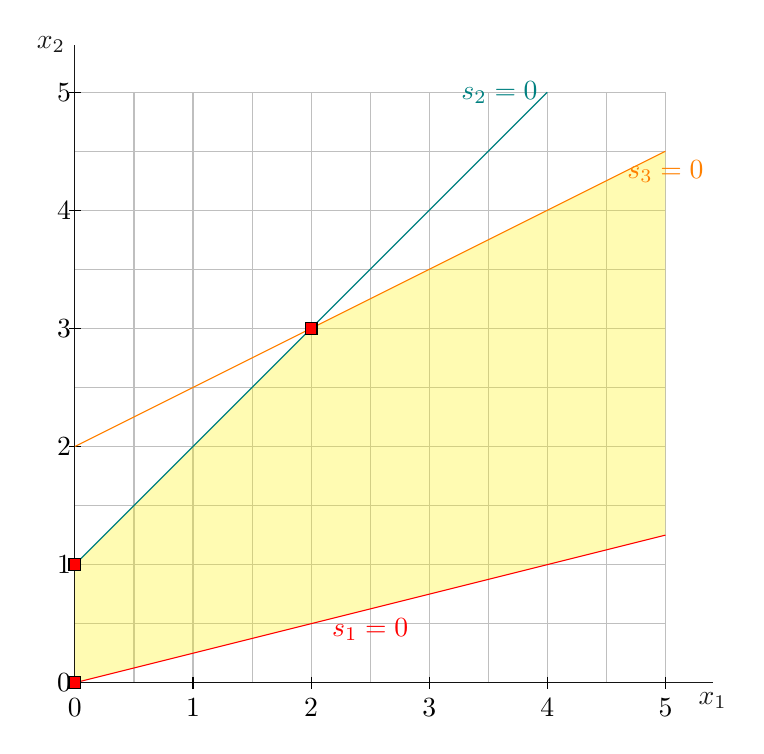
\begin{tikzpicture} [scale=1.5]
    \draw[gray!50, thin, step=.5] (0,0) grid (5,5);
    \draw[opacity=0.9] (0,0) -- (5.4,0) node[below] {$x_1$};
    \draw[opacity=0.9] (0,0) -- (0,5.4) node[left] {$x_2$}; % option \draw[very thick,->]

    \foreach \x in {0,...,5} \draw (\x,0.05) -- (\x,-0.05) node[below] {\x};
    \foreach \y in {0,...,5} \draw (-0.05,\y) -- (0.05,\y) node[left] {\y};

    \fill[yellow,opacity=0.3] (0,0) -- (0,1) -- (2,3) -- (5,4.5) --(5,1.25)-- cycle;

    \draw [red](0,0) -- node[below] {$s_1=0$} (5, 1.25);
    \draw [teal] (0,1)  --  (4,5) node[left, sloped] {$s_2=0$};
    \draw [orange](0,2) --  (5,4.5) node[below, sloped] {$s_3=0$}; %node[above right ,sloped] 
	\filldraw[fill=red] (-0.05,-0.05) rectangle (0.05,0.05);
	\filldraw[fill=red] (-0.05,.95) rectangle (0.05,1.05);
	\filldraw[fill=red] (1.95,2.95) rectangle (2.05,3.05);
\end{tikzpicture} \end{center} 
\end{minipage}

\begin{center}  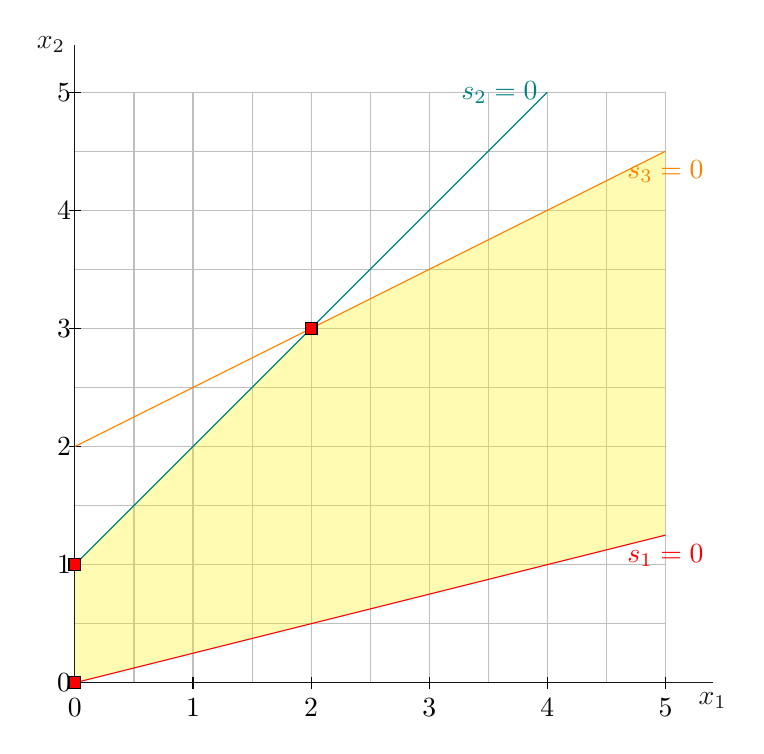
\begin{tikzpicture} [scale=1.5]
    \draw[gray!50, thin, step=.5] (0,0) grid (5,5);
    \draw[opacity=0.9] (0,0) -- (5.4,0) node[below] {$x_1$};
    \draw[opacity=0.9] (0,0) -- (0,5.4) node[left] {$x_2$}; % option \draw[very thick,->]

    \foreach \x in {0,...,5} \draw (\x,0.05) -- (\x,-0.05) node[below] {\x};
    \foreach \y in {0,...,5} \draw (-0.05,\y) -- (0.05,\y) node[left] {\y};

    \fill[yellow,opacity=0.3] (0,0) -- (0,1) -- (2,3) -- (5,4.5) --(5,1.25)-- cycle;

\draw[domain=0:4,smooth,variable=\x, teal] plot ({\x},{\x+1}) node[left] {$s_2=0$};
\draw[domain=0:5,smooth,variable=\x, red] plot ({\x},{\x*1/4}) node[below] {$s_1=0$};
%    \draw [red](0,0) -- node[below] {$s_1=0$} (5, 1.25);
    %\draw [teal] (0,1)  --  (4,5) node[left, sloped] {$s_2=0$};
    \draw [orange](0,2) --  (5,4.5) node[below, sloped] {$s_3=0$}; %node[above right ,sloped] 
	\filldraw[fill=red] (-0.05,-0.05) rectangle (0.05,0.05);
	\filldraw[fill=red] (-0.05,.95) rectangle (0.05,1.05);
	\filldraw[fill=red] (1.95,2.95) rectangle (2.05,3.05);
\end{tikzpicture} \end{center} 

% \draw[scale=0.5,domain=-3:3,smooth,variable=\x,blue] plot ({\x},{\x*\x});


\medskip E.g., consider the $s_3=0$ (orange) line, to find the extreme direction start at extreme point (2,3) and find another feasible point on the orange line, say (4,4) and subtract (2,3) from (4,4), which yields (2,1). 

\medskip This is related to the slope in two-dimensions, as discussed in class, the rise is 1 and the run is 2. So this direction has a slope of 1/2, but this does not carry over easily to higher dimensions where directions cannot be defined by a single number. 

\medskip To find the extreme directions we can change the right-hand-side to $\mathbf{b} = \mathbf{0}$, which forms a polyhedral cone (in yellow), and then add the constraint $x_1 + x_2 = 1$. The intersection of the cone and  $x_1 + x_2 = 1$ form a line segment.

\begin{minipage}[t][][b]{.4\linewidth} \vspace{0mm}
\begin{align*}
\mbox{max~~} & z = -5x_1 - x_2  \\
\mbox{s.t.~~} & x_1 - 4x_2 +s_1 = 0  \\
& -x_1 + x_2 + s_2 = 0 \\
& -x_1 + 2x_2 +s_3 = 0 \\
& x_1 + x_2 = 1 \\
& x_1, x_2, s_1, s_2, s_3 \ge 0.
\end{align*}
\end{minipage}%
\begin{minipage}[t][][b]{.6\linewidth}
\begin{center} 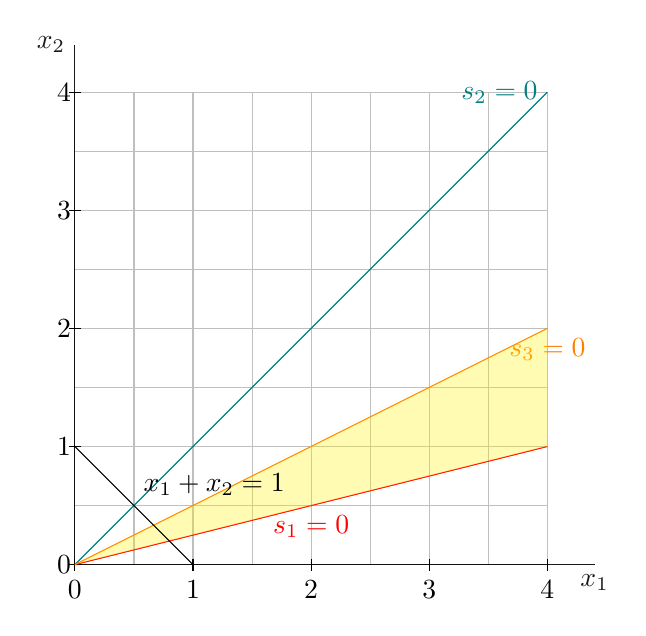
\begin{tikzpicture} [scale=1.5]
\draw[gray!50, thin, step=.5] (0,0) grid (4,4);
\draw[opacity=0.9] (0,0) -- (4.4,0) node[below] {$x_1$};
\draw[opacity=0.9] (0,0) -- (0,4.4) node[left] {$x_2$}; % option \draw[very thick,->]

\foreach \x in {0,...,4} \draw (\x,0.05) -- (\x,-0.05) node[below] {\x};
\foreach \y in {0,...,4} \draw (-0.05,\y) -- (0.05,\y) node[left] {\y};
        
\draw [red](0, 0) -- node[below] {$s_1=0$} (4, 1);
\draw [teal] (0,0)  -- (4,4) node[left, sloped] {$s_2=0$};
\draw [orange](0,0) -- (4,2) node[below, sloped] {$s_3=0$}; 
\fill[yellow,opacity=0.3] (0,0) -- (4,2) -- (4,1) --  cycle; % \draw [orange!50!blue] 

\draw [black] (0,1)  -- node[above right] {$x_1+x_2 = 1$} (1,0); 
\end{tikzpicture} \end{center} 
\end{minipage}



\begin{center} 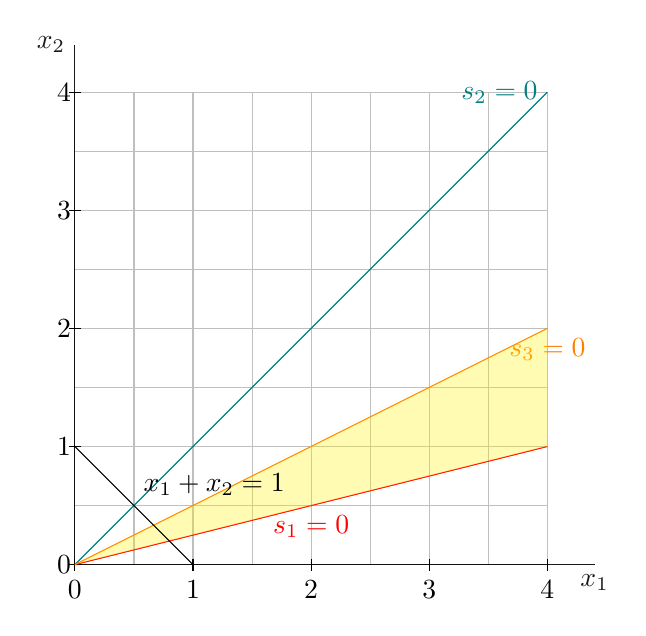
\begin{tikzpicture} [scale=1.5]
\draw[gray!50, thin, step=.5] (0,0) grid (4,4);
\draw[opacity=0.9] (0,0) -- (4.4,0) node[below] {$x_1$};
\draw[opacity=0.9] (0,0) -- (0,4.4) node[left] {$x_2$}; % option \draw[very thick,->]

\foreach \x in {0,...,4} \draw (\x,0.05) -- (\x,-0.05) node[below] {\x};
\foreach \y in {0,...,4} \draw (-0.05,\y) -- (0.05,\y) node[left] {\y};
        
\draw [red](0, 0) -- node[below] {$s_1=0$} (4, 1);
\draw [teal] (0,0)  -- (4,4) node[left, sloped] {$s_2=0$};
\draw [orange](0,0) -- (4,2) node[below, sloped] {$s_3=0$}; 
\fill[yellow,opacity=0.3] (0,0) -- (4,2) -- (4,1) --  cycle; % \draw [orange!50!blue] 

\draw [black] (0,1)  -- node[above right] {$x_1+x_2 = 1$} (1,0); 
\end{tikzpicture} \end{center} 


\medskip Magnifying for clarity, and removing the $s_2=0$ (teal) line, as it is redundant, and marking the extreme points of the new feasible region, (4/5, 1/5) and (2/3, 1/3), with red boxes, we have:

\begin{center}  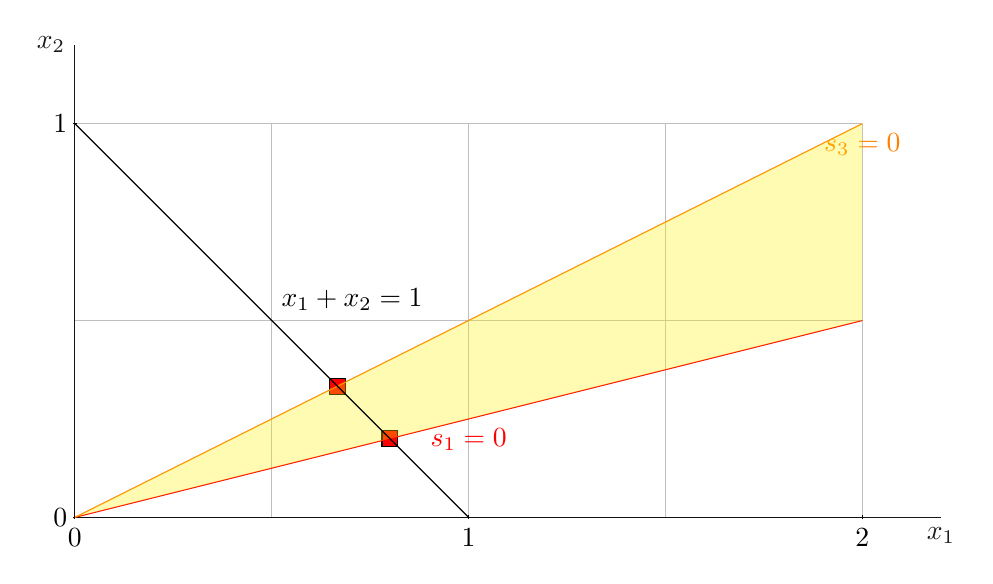
\begin{tikzpicture} [x=50mm, y=50mm] [scale=1.5]
\draw[gray!50, thin, step=.5] (0,0) grid (2,1);
\draw[opacity=0.9] (0,0) -- (2.2,0) node[below] {$x_1$};
\draw[opacity=0.9] (0,0) -- (0,1.2) node[left] {$x_2$}; % option \draw[very thick,->]

\foreach \x in {0,...,2} \draw (\x,0.005) -- (\x,-0.005) node[below] {\x};
\foreach \y in {0,...,1} \draw (-0.005,\y) -- (0.005,\y) node[left] {\y};

\filldraw[fill=red] (0.8-0.02,0.2-0.02) rectangle (0.8+0.02,0.2+0.02);
\filldraw[fill=red] (0.667-0.02,0.333-0.02) rectangle (0.667+0.02,0.333+0.02);

\draw [red](0, 0) -- node[below] {$s_1=0$} (2, .5);
\draw [orange](0,0) -- (2,1) node[below, sloped] {$s_3=0$}; 
\fill[yellow,opacity=0.3] (0,0) -- (2,.5) -- (2,1) --  cycle; % \draw [orange!50!blue] 
\draw [black] (0,1)  -- node[above right] {$x_1+x_2 = 1$} (1,0); 
\end{tikzpicture} \end{center} 

The extreme directions are thus (4/5, 1/5) and (2/3, 1/3). \\

{\bf Representation Theorem:} Let  $\mathbf{x_1}, \mathbf{x_2},\cdots \mathbf{x_k}$ be the set of extreme points of $\mathcal{S}$, and if $\mathcal{S}$ is unbounded, $\mathbf{d_1}, \mathbf{d_2},\cdots \mathbf{d_l}$ be the set of extreme directions. Then any $\mathbf{x} \in \mathcal{S}$ is equal to a convex combination of the extreme points and a non-negative linear combination of the extreme directions: $\mathbf{x} = \sum_{j=1}^k \lambda_j \mathbf{x_j} + \sum_{j=1}^l \mu_j \mathbf{d_j}$, where $\sum_{j=1}^k \lambda_j = 1$, $\lambda_j \ge 0,~\forall  j=1,2,\cdots,k$, and $\mu_j \ge 0,~\forall j=1,2,\cdots,l$.

 \begin{minipage}[t][][b]{.4\linewidth}
\begin{align*}
\mbox{max~~} & z = -5x_1 - x_2  \\\
\mbox{s.t.~~} & x_1 - 4x_2 +s_1 = 0  \\
& -x_1 + x_2 + s_2 = 1 \\
& -x_1 + 2x_2 +s_3 = 4 \\
& x_1, x_2, s_1, s_2, s_3 \ge 0.
\end{align*}
\end{minipage}%
\begin{minipage}[t][][b]{.6\linewidth}
\begin{center}  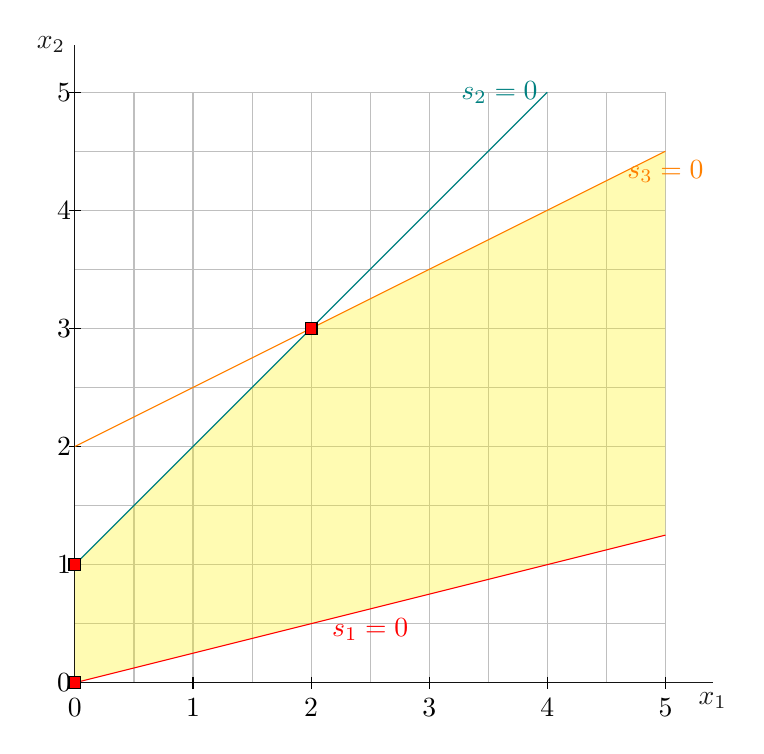
\begin{tikzpicture} [scale=1.5]
    \draw[gray!50, thin, step=.5] (0,0) grid (5,5);
    \draw[opacity=0.9] (0,0) -- (5.4,0) node[below] {$x_1$};
    \draw[opacity=0.9] (0,0) -- (0,5.4) node[left] {$x_2$}; % option \draw[very thick,->]

    \foreach \x in {0,...,5} \draw (\x,0.05) -- (\x,-0.05) node[below] {\x};
    \foreach \y in {0,...,5} \draw (-0.05,\y) -- (0.05,\y) node[left] {\y};

    \fill[yellow,opacity=0.3] (0,0) -- (0,1) -- (2,3) -- (5,4.5) --(5,1.25)-- cycle;

    \draw [red](0,0) -- node[below] {$s_1=0$} (5, 1.25);
    \draw [teal] (0,1)  --  (4,5) node[left, sloped] {$s_2=0$};
    \draw [orange](0,2) --  (5,4.5) node[below, sloped] {$s_3=0$}; %node[above right ,sloped] 
	\filldraw[fill=red] (-0.05,-0.05) rectangle (0.05,0.05);
	\filldraw[fill=red] (-0.05,.95) rectangle (0.05,1.05);
	\filldraw[fill=red] (1.95,2.95) rectangle (2.05,3.05);
\end{tikzpicture} \end{center} 
\end{minipage}

Represent point (1/2, 1) as a convex combination of the extreme points of the above LP.  Find $\lambda$s to solve the following system of equations:

$$\lambda_1 \left[
  \begin{array}{c}
  0 \\
  0 \\
  \end{array} \right]+
 \lambda_2 \left[
  \begin{array}{c}
  0 \\
  1 \\
  \end{array} \right] +
 \lambda_3 \left[
  \begin{array}{c}
  2 \\
  3 \\
  \end{array} \right]  =
 \left[
  \begin{array}{c}
  1/2 \\
  1 \\
  \end{array} \right] 
$$


\newpage The Variable (Canonical Form) and Requirement Space 

\begin{minipage}[t][][b]{.4\linewidth}
\begin{align*}
\mbox{max~~} & z = 2x_1 + x_2  \\\
\mbox{s.t.~~} & x_1 - x_2 +s_1 =  2  \\
& x_1 + x_2 +s_2  = 3 \\
& x_1, x_2, s_1 , s_2  \ge 0.
\end{align*}
\end{minipage}%
\begin{minipage}[t][][b]{.6\linewidth}
\begin{center}  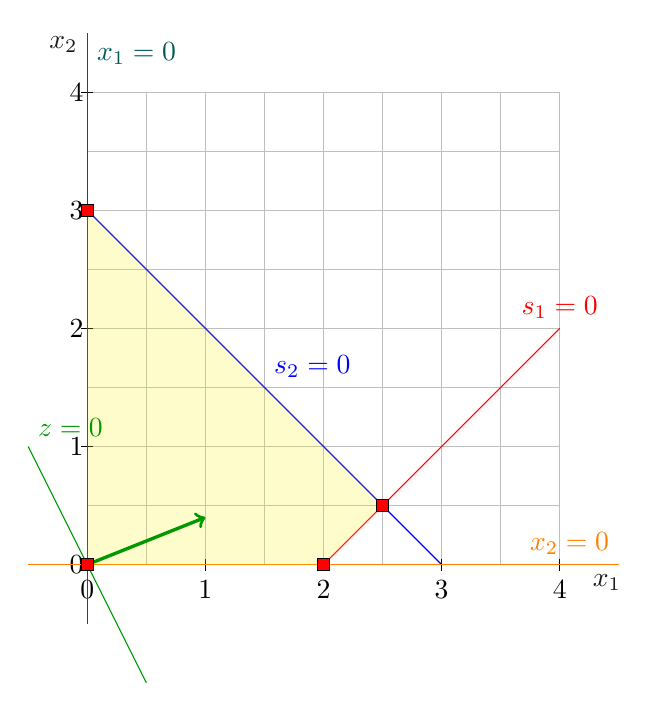
\begin{tikzpicture} [scale=1.5]
\draw[gray!50, thin, step=.5] (0,0) grid (4,4);
\draw[opacity=0.9] (0,0) -- (4.4,0) node[below] {$x_1$};
\draw[opacity=0.9] (0,0) -- (0,4.4) node[left] {$x_2$};

\foreach \x in {0,...,4} \draw (\x,0.05) -- (\x,-0.05) node[below] {\x};
\foreach \y in {0,...,4} \draw (-0.05,\y) -- (0.05,\y) node[left] {\y};

\draw [red](2, 0) --  (4, 2) node[above] {$s_1= 0$};
\draw [blue] (0,3)  -- node[above right] {$s_2=0$} (3,0) ;
\draw [teal!70!black](0,-.5) --  (0,4.5) node[below right] {$x_1=0$}; 
\draw [orange](-.5,0) --  (4.5,0) node[above left] {$x_2=0$}; 

\fill[yellow,opacity=0.2] (0,0) -- (2,0) -- (2.5,0.5) -- (0,3) -- cycle;

\draw [green!60!black] (-0.5, 1)  node[above right] {$z=0$} --  (0.5, -1)  ; % o.f.
\draw [green!60!black, very thick,->](0,0) -- (0+1, 0+2/5); % gradient

\filldraw[fill=red] (-0.05,-0.05) rectangle (0.05,0.05);
\filldraw[fill=red] (2.45,0.45) rectangle (2.55,0.55);
\filldraw[fill=red] (1.95,-0.05) rectangle (2.05,0.05);
\filldraw[fill=red] (-0.05,2.95) rectangle (0.05,3.05);    
\end{tikzpicture} \end{center} 
\end{minipage}



\begin{minipage}[t][][b]{.4\linewidth}
\begin{align*}
\mbox{max~~} & z = 2x_1 + x_2  \\\
\mbox{s.t.~~} & x_1 - x_2 +s_1 =  2  \\
& x_1 + x_2 +s_2  = 3 \\
& x_1, x_2, s_1 , s_2  \ge 0.
\end{align*}
\end{minipage}%
\begin{minipage}[t][][b]{.6\linewidth}
\begin{center}  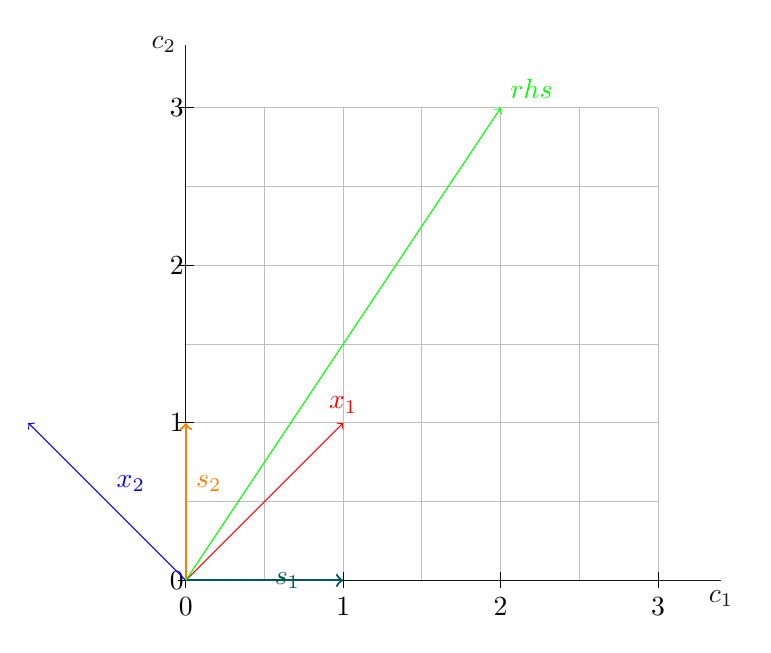
\begin{tikzpicture}[x=20mm, y=20mm] [scale=1.5]  % requirement space
\draw[gray!50, thin, step=.5] (0,0) grid (3,3);
\draw[opacity=0.9] (0,0) -- (3.4,0) node[below] {$c_1$};
\draw[opacity=0.9] (0,0) -- (0,3.4) node[left] {$c_2$};

\foreach \x in {0,...,3} \draw (\x,0.05) -- (\x,-0.05) node[below] {\x};
\foreach \y in {0,...,3} \draw (-0.05,\y) -- (0.05,\y) node[left] {\y};

\draw [red,->](0, 0) --  (1, 1) node[above] {$x_1$};
\draw [blue,->] (0,0)  -- node[above right] {$x_2$} (-1,1) ;
\draw [thick, teal!70!black,->](0,0) -- node[right] {$s_1$} (1,0); 
\draw [thick, orange,->](0,0) -- node[above right] {$s_2$} (0,1); 
\draw [green,->] (0, 0)  --  (2,3) node[above right] {$rhs$}   ; 
\end{tikzpicture} \end{center} 
\end{minipage}


\newpage \underline {\bf Tableaus} \\  % introducing tableaus

After putting an LP into standard form, we can put the system of equations into a table form, the ``tableau". \\

\begin{minipage}[t][][b]{.4\linewidth} \vspace{-5mm}
\begin{align*}
\mbox{max~~} & z = 2x_1 + x_2  \\
\mbox{s.t.~~} & x_1 - x_2 +s_1 =  2  \\
& x_1 + x_2 +s_2  = 3 \\
& x_1, x_2, s_1 , s_2  \ge 0.
\end{align*}
\end{minipage}%
\begin{minipage}[t][][b]{.6\linewidth}
\begin{center} \begin{tabular} {l|c||c|c|c|c|c|}  \cline{2-7}
max & $z$	& $x_1$ & $x_2$  & $x_3$	& $x_4$	& $rhs$ \\ \cline{2-7}
(r0 - z)	    & 1		& -2        &  -1        &	 0 	    &	  0		&   0    \\ \cline{2-7}
(r1 - $x_3$)			& 0		&	 1        &     -1     &	 1 			&	  0 		&	  2   \\
(r2 - $x_4$)			& 0		&	  1       &	    1    &	 0 		&	  1 		&	   3   \\ \cline{2-7}
\end{tabular} \end{center}
\end{minipage} \\
 
\bigskip Why are the coefficients negative in row zero, we change $z = 2x_1 + x_2 $ to $z - 2x_1 - x_2 =0$ so we have only constants on the right-hand-side (rhs). \\

This tableau represents a basic solution, because it contains an identity matrix.  The basic variables are those variables having columns in the identity matrix (here, $x_3$ and $x_4$), and it is feasible because the rhs for row $1-m$ are non-negative. \\

We can consider $z$ a permanent member of an expanded basis if we treat row zero like any other row (although the rhs of row~0 can be negative).

\newpage \underline{\bf Basic Solutions and Extreme Points}

\begin{minipage}[t][][b]{.55\linewidth} \vspace{2mm}
\begin{center} \begin{tabular} {l|c||c|c|c|c|c|}  \cline{2-7}
max & $z$	& $x_1$ & $x_2$  & $x_3$	& $x_4$	& $rhs$ \\ \cline{2-7}
(r0 - z)	    & 1		& -2        &  -1        &	 0 	    &	  0		&   0    \\ \cline{2-7}
(r1 - $x_3$)			& 0		&	 1        &     -1     &	 1 			&	  0 		&	  2   \\
(r2 - $x_4$)			& 0		&	  1       &	    1    &	 0 		&	  1 		&	   3   \\ \cline{2-7}
\end{tabular} \end{center}
\end{minipage}%
\begin{minipage}[t][][b]{.45\linewidth}
\begin{center}  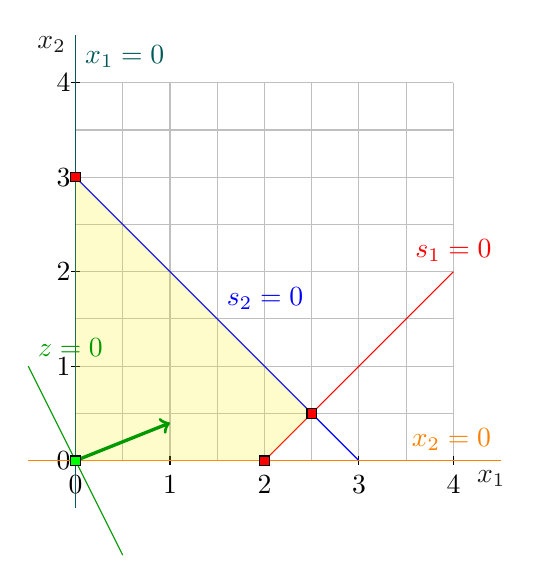
\begin{tikzpicture} [scale=1.2]
\draw[gray!50, thin, step=.5] (0,0) grid (4,4);
\draw[opacity=0.9] (0,0) -- (4.4,0) node[below] {$x_1$};
\draw[opacity=0.9] (0,0) -- (0,4.4) node[left] {$x_2$};

\foreach \x in {0,...,4} \draw (\x,0.05) -- (\x,-0.05) node[below] {\x};
\foreach \y in {0,...,4} \draw (-0.05,\y) -- (0.05,\y) node[left] {\y};

\draw [red](2, 0) --  (4, 2) node[above] {$s_1= 0$};
\draw [blue] (0,3)  -- node[above right] {$s_2=0$} (3,0) ;
\draw [teal!70!black](0,-.5) --  (0,4.5) node[below right] {$x_1=0$}; 
\draw [orange](-.5,0) --  (4.5,0) node[above left] {$x_2=0$}; 

\fill[yellow,opacity=0.2] (0,0) -- (2,0) -- (2.5,0.5) -- (0,3) -- cycle;

\draw [green!60!black] (-0.5, 1)  node[above right] {$z=0$} --  (0.5, -1)  ; % o.f.
\draw [green!60!black, very thick,->](0,0) -- (0+1, 0+2/5); % gradient

\filldraw[fill=green] (-0.05,-0.05) rectangle (0.05,0.05);
\filldraw[fill=red] (2.45,0.45) rectangle (2.55,0.55);
\filldraw[fill=red] (1.95,-0.05) rectangle (2.05,0.05);
\filldraw[fill=red] (-0.05,2.95) rectangle (0.05,3.05);    
\end{tikzpicture} \end{center} 
\end{minipage}

Here the basic variables are $x_3 = 2$ and $x_4=3$, and the $z$-value of objective function value is 0. \\

Let's go to the extreme point (2,0) which has basic variables $x_1$ and $x_4$ (this new extreme point is adjacent to the extreme point (0,0). Why? \\
% they share an edge, and are defined by the same n-1 hypeplanes.
\begin{center} \begin{tabular} {l|c||c|c|c|c|c|}  \cline{2-7}
max & $z$	& $x_1$ & $x_2$  & $x_3$	& $x_4$	& $rhs$ \\ \cline{2-7}
(r0 - z)	    & 1		& -2        &  -1        &	 0 	    &	  0		&   0    \\ \cline{2-7}
(r1 - $x_3$)			& 0		&	 1        &     -1     &	 1 			&	  0 		&	  2   \\
(r2 - $x_4$)			& 0		&	  1       &	    1    &	 0 		&	  1 		&	   3   \\ \cline{2-7}
\end{tabular} \end{center}

First get a 1 coefficent in row~1 in the  $x_1$ column by multiplying row~1 by a scalar (no action needed, already equals one).\\
 
\begin{center} \begin{tabular} {l|c||c|c|c|c|c|}  \cline{2-7}
max 			& $z$	& $x_1$ & $x_2$  & $x_3$	& $x_4$	& $rhs$ \\ \cline{2-7}
(r0 - z)	    & 1		& -2        &  -1        &	 0 	    &	  0		&   0    \\ \cline{2-7}
(r1 - $x_3$)	& 0		&	 1        &     -1     &	 1 			&	  0 		&	  2   \\
(r2 - $x_4$)	& 0		&	  1       &	    1    &	 0 		&	  1 		&	   3   \\ \cline{2-7}
\end{tabular} \end{center}

Then use row~1 to zero out the row~0 coefficient for $x_1$ by multiplying row~1 by 2 and adding it to row~0 to get a new row~0.\\


\begin{center} \begin{tabular} {l|c||c|c|c|c|c|}  \cline{2-7}
max 			& $z$	& $x_1$ & $x_2$  & $x_3$	& $x_4$	& $rhs$ \\ \cline{2-7}
(r0 -z)	    	& 1		& 0     & -3     &	 2 	&	  0	&   4    \\ \cline{2-7}
(r1 - $x_3$)	& 0		& 1     & -1     &	 1 	&	  0 &	  2   \\
(r2 - $x_4$)	& 0		& 1     &  1    &	 0 	&	  1 &	   3   \\ \cline{2-7}
\end{tabular} \end{center}

Lastly use row~1 to zero out the row~20 coefficient for $x_1$ by multiplying row~1 by -1 and adding it to row~2 to get a new row 2. \\


\begin{center} \begin{tabular} {l|c||c|c|c|c|c|}  \cline{2-7}
max 			& $z$	& $x_1$ & $x_2$  & $x_3$	& $x_4$	& $rhs$ \\ \cline{2-7}
(r0 -z)	    	& 1		& 0     & -3     &	 2 	&	  0	&   4    \\ \cline{2-7}
(r1 - $x_3$)	& 0		& 1     & -1     &	 1 	&	  0 &	2   \\
(r2 - $x_4$)	& 0		& 0     &  2    &	-1 	&	  1 &	1   \\ \cline{2-7}
\end{tabular} \end{center}

\newpage The nonbasic variables for this tableau are $x_2$ and $x_3$, so we can graph the new LP in the nonbasic variable space.

\begin{minipage}[t][][b]{.55\linewidth} \vspace{2mm}
\begin{center} \begin{tabular} {l|c||c|c|c|c|c|}  \cline{2-7}
max 			& $z$	& $x_1$ & $x_2$  & $x_3$	& $x_4$	& $rhs$ \\ \cline{2-7}
(r0 -z)	    	& 1		& 0     & -3     &	 2 	&	  0	&   4    \\ \cline{2-7}
(r1 - $x_3$)	& 0		& 1     & -1     &	 1 	&	  0 &	2   \\
(r2 - $x_4$)	& 0		& 0     &  2    &	-1 	&	  1 &	1   \\ \cline{2-7}
\end{tabular} \end{center}
\end{minipage}%
\begin{minipage}[t][][b]{.45\linewidth}
\begin{center}  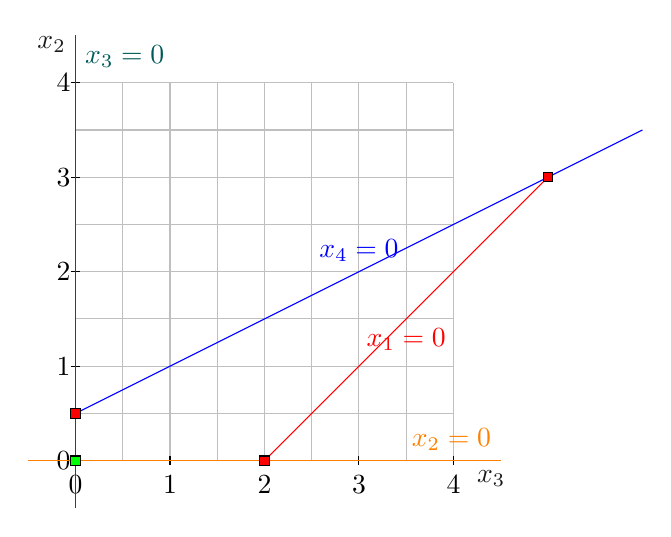
\begin{tikzpicture} [scale=1.2]
\draw[gray!50, thin, step=.5] (0,0) grid (4,4);
\draw[opacity=0.9] (0,0) -- (4.4,0) node[below] {$x_3$};
\draw[opacity=0.9] (0,0) -- (0,4.4) node[left] {$x_2$};

\foreach \x in {0,...,4} \draw (\x,0.05) -- (\x,-0.05) node[below] {\x};
\foreach \y in {0,...,4} \draw (-0.05,\y) -- (0.05,\y) node[left] {\y};

\draw [red](2, 0) --  node[below] {$x_1= 0$} (5, 3) ;
\draw [blue] (0,0.5)  -- node[above] {$x_4=0$} (6,3.5) ;
\draw [teal!70!black](0,-.5) --  (0,4.5) node[below right] {$x_3=0$}; 
\draw [orange](-.5,0) --  (4.5,0) node[above left] {$x_2=0$}; 

%\fill[yellow,opacity=0.2] (0,0) -- (2,0) -- (2.5,0.5) -- (0,3) -- cycle;

%\draw [green!60!black] (-0.5, 1)  node[above right] {$z=0$} --  (0.5, -1)  ; % o.f.
%\draw [green!60!black, very thick,->](0,0) -- (0+1, 0+2/5); % gradient

\filldraw[fill=green] (-0.05,-0.05) rectangle (0.05,0.05);
\filldraw[fill=red] (1.95,-0.05) rectangle (2.05,0.05);
\filldraw[fill=red] (4.95,2.95) rectangle (5.05,3.05);
\filldraw[fill=red] (-0.05,0.45) rectangle (0.05,0.55);    
\end{tikzpicture} \end{center} 
\end{minipage}



\newpage \underline{\bf Matrix Math}

\bigskip  An $m \times n$ matrix is an array of real numbers with $m$ rows and $n$ columns. Any matrix can be represented by its constituent set of row or column vectors. \\

$\mathbf{A} =
\left[
  \begin{array}{cc}
    1 & 3 \\
    6 & 4 \\
  \end{array}
\right]     =
\left[
  \begin{array}{cc}
  \mathbf{a_1} & \mathbf{a_2} \\
  \end{array}
\right]     =
\left[
  \begin{array}{c}
  \mathbf{a^1} \\
  \mathbf{a^2} \\
  \end{array}
\right], $ \\

\noindent where
$\mathbf{a_1} =
\left[
  \begin{array}{c}
  1 \\
  6 \\
  \end{array}
\right],~ \mathbf{a_2} =
\left[
  \begin{array}{c}
  3 \\
  4 \\
  \end{array} \right],~
\mathbf{a^1} =
\left[\begin{array}{cc}
  1 & 3 \\
\end{array} \right],~ $and$~
\mathbf{a^2} = \left[\begin{array}{cc}
  6 & 4 \\
\end{array} \right]$.  Additionally, $a_{11} = 1$, $a_{12} = 3$, $a_{21} = 6$, $a_{22} = 4$. \\

{\bf Matrix Addition:} Two matrices of the same dimension can be added componentwise, thus $\mathbf{C} = \mathbf{A} + \mathbf{B}$ means that $c_{ij} = a_{ij} + b_{ij}$. \\

{\bf Scalar Multiplication:} Just like it sounds. If $k$ is a scalar, then $k\mathbf{A}$ means that every component of $\mathbf{A}$ is multiplied by $k$. \\

{\bf Matrix Multiplication:} $\mathbf{A}$ is a $m \times n$ matrix and $\mathbf{B}$ is a $p \times q$ matrix.  $\mathbf{AB}$ (matrix multiplication) is only defined if $n = p$ and the result is a $m \times q$ matrix, $\mathbf{BA}$ is only defined if $q = m$ and the result is a $p \times n$. $\mathbf{AB}$ is not necessarily equal to $\mathbf{BA}$, thus $\mathbf{C} = \mathbf{AB}$ where $c_{ij} = \sum_{k=1}^n a_{ik}b_{kj},~ i=1,\cdots,m,~ j=1,\cdots,p$, e.g., $c_{11}$ is the sum of the the componentwise multiplication of the first row of $\mathbf{A}$ and the first column of $\mathbf{B}$. \\

{\bf Identity Matrix:} A square matrix (denoted by $\mathbf{I}$) with all zero components, except for the diagonal: \\
$\left[ \begin{array}{ccc}
     1 & 0 & 0 \\
     0 & 1 & 0 \\
     0 & 0 & 1 \\
\end{array} \right]$ \\


{\bf Elementary Matrix Operations:}
These operations are used to solve systems of linear equations or inverting a matrix. The three operations are as follows (for any matrix $\mathbf{A}$):

\begin{itemize}
\item Interchange two rows of $\mathbf{A}$.
\item Multiply a row by a nonzero scalar.
\item Replace row $i$ with row $i$ plus row $j$ multiplied by a nonzero scalar.
\end{itemize}

\bigskip {\bf Inverting a Matrix:}

\bigskip $\mathbf{A} = \left[
   \begin{array}{ccc}
     3 & 9 & 2 \\
     1 & 1 & 1 \\
     5 & 4 & 7 \\
   \end{array} \right]~and~\mathbf{A^{-1}} = \left[
   \begin{array}{ccc}
     -\frac{3}{11} & 5 & -\frac{7}{11} \\
     \frac{2}{11} & -1 & \frac{1}{11} \\
     \frac{1}{11} & -3 & \frac{6}{11} \\
   \end{array} \right]$

\bigskip To find $\mathbf{A^{-1}}$ using elementary row operations to transform $\mathbf{A}$ into an identity matrix, while performing these same operations on the attached identity matrix.

\bigskip $\left[ \begin{array}{ccc|ccc} \nonumber
         3 & 9 & 2 & 1 & 0 & 0 \\
         1 & 1 & 1 & 0 & 1 & 0 \\
         5 & 4 & 7 & 0 & 0 & 1 \\
\end{array} \right] \Rightarrow
\left[ \begin{array}{ccc|ccc} \nonumber
         1 & 0 & 0 & -\frac{3}{11} & 5 & -\frac{7}{11} \\
         0 & 1 & 0 & \frac{2}{11} & -1 & \frac{1}{11} \\
         0 & 0 & 1 & \frac{1}{11} & -3 & \frac{6}{11} \\
\end{array} \right].$ \\

{\bf Rank of a Matrix:} $\mathbf{A}$ is a $m \times n$ matrix then rank$(\mathbf{A}) \le min\{m,~n\}$, if rank$(\mathbf{A}) = min\{m,~n\}$, then $\mathbf{A}$ is of full rank.  If $\mathbf{A}$ is not full rank, but of rank $k$, where $k < min\{m,~n\}$, then using the elementary row operations, we can transform $\mathbf{A}$ to the following:
$\left[
   \begin{array}{cc}
     \mathbf{I_k} & \mathbf{Q}  \\
     0            & 0 \\
\end{array} \right]$

\begin{comment}
\bigskip {\bf Simultaneous Linear Equations}

\bigskip Consider the system $\mathbf{A} \mathbf{x} = \mathbf{b}$, where $\mathbf{A}$ is a $m \times n$ matrix of rank $m$ and $m \le n$. We can partition $\mathbf{A}$ such that $\mathbf{A} = [\mathbf{B}, \mathbf{N}]$, where
\begin{itemize}
\item the {\it basis matrix} $\mathbf{B}$ is a nonsingular (i.e., it consists of $m$ linearly dependent columns of $\mathbf{A}$) $m \times m$ matrix.
\item the {\it nonbasic matrix} $\mathbf{N}$ is a $m \times n-m$ matrix
\end{itemize}

The vector $\mathbf{x}$ can be divided in a similar way (each column corresponds to a variable), yielding $\mathbf{x_B}$ and $\mathbf{x_N}$. \\

We can write our system as follows: 
$$\mathbf{B} \mathbf{x_B} + \mathbf{N} \mathbf{x_N} = \mathbf{b}.$$ 
$$\mathbf{B} \mathbf{x_B}  = \mathbf{b}-  \mathbf{N} \mathbf{x_N}.$$ 
Premultiplying by $\mathbf{B^{-1}}$ yields:  
$$\mathbf{x_B} = \mathbf{B^{-1}}\mathbf{b} - \mathbf{B^{-1}} \mathbf{N} \mathbf{x_N}.$$ 

By setting $\mathbf{x_N} = \mathbf{0}$ and solving we (potentially) find a {\it basic feasible solution} to the system, which corresponds to an extreme point of the feasible region, remember that the nonbasic variables $\mathbf{x_N} = \mathbf{0}$ represent the defining hyperplanes for a solution. For any set of $m$ variables, the result can be:

\begin{enumerate}
\item a basic feasible solution, $\mathbf{x_B} \ge \mathbf{0}$.
\item a basic infeasible solution, some $x \in \mathbf{x_B} \le 0$.
\item a set of linearly dependent columns that does not span the $m$-space.
\end{enumerate}

For this system there are possibly ${n \choose m}$ basic solutions, that is, the number of basic feasible solutions is bounded by $n!/m!(n-m)!$ from above.  \\




\bigskip The following are the four possible cases for an LP:
%Describe (0.5, 1) in terms of extreme points and directions.
%Describe (3, 2) in terms of extreme points and directions.



\begin{itemize}
\item Unique optimal solution 
\item Multiple optimal solutions
\item Unbounded optimal objective value
\item Empty feasible region (an infeasible LP)
\end{itemize}
\end{comment}

\subsection{Linear Optimization Theory} %By Douglas Bish
%The text is licensed under the
%\href{http://creativecommons.org/licenses/by-sa/4.0/}{Creative Commons
%Attribution-ShareAlike 4.0 International License}.
%
%This file has been modified by Robert Hildebrand 2020.  
%CC BY SA 4.0 licence still applies.


Consider an arbitrary LP, which we will call the primal ($P$): 
$$(P):\max \{\mathbf{cx}: \mathbf{Ax} \le \mathbf{b}, \mathbf{x} \ge 0\},$$ 
where $\mathbf{A}$ is an $m\times n$ matrix, and $\mathbf{x}$ is a $n$ element column vector.  Every prmal LP has a related LP, which we call the dual, the dual of ($P$) is:
$$(D):\min \{\mathbf{wb}: \mathbf{wA} \ge \mathbf{c}, \mathbf{w} \ge 0\}.$$ 

Before we discuss properties of duality, and why it is important, we start with how to formulate the dual for any given LP. If the LP has a different form like $P$, we find the dual based on the $P$ and $D$ example above.  If the LP does not have this form, we can transform it to this form, or use the rules in the following table, first noting that:

\begin{itemize}
\item The dual of problem $D$ is problem $P$.
\item Each primal constraint has an associated dual variable ($w_i$) and each dual constraint has an associated primal variable ($x_i$).
\item When the primal is a maximization, the dual is a minimization, and vice versa.
\end{itemize}

\begin{align*}
\max~& {\bf cx}:~~~~~~~~~~~~			& \min~ & {\bf wb}:  \\
&{\bf a_{1*}x} \le b_1~(w_1 \ge 0)   &     & {\bf wa_{*1}} \ge c_1~(x_1 \ge 0) \\ 
&{\bf a_{2*}x} = b_2~(w_2~urs)       &     & {\bf wa_{*2}} = c_2~(x_2~urs) \\
&{\bf a_{3*}x} \ge b_3~(w_3 \le 0) &        & {\bf wa_{*3}} \le c_3~(x_3 \le 0) \\
&\vdots 							   &      & \vdots \\ 
&x_1 \ge 0, x_2~urs, x_3 \le 0, \cdots &  	 & w_1 \ge 0, w_2~urs, w_3 \le 0,\cdots   
\end{align*}


To illustrate the relationship between the primal and dual, consider this production problem we previously formulated: \\

{\bf Production Problem:} You have 21 units of transparent aluminum alloy (TAA), LazWeld1, a joining robot leased for 23 hours, and CrumCut1, a cutting robot leased for 17 hours of aluminum cutting. You also have production code for a bookcase, desk, and cabinet, along with commitments to buy any of these you can produce for \$18,  \$16, and  \$10 apiece, respectively.  A bookcase requires 2 units of TAA, 3 hours of joining, and 1 hour of cutting, a desk requires 2 units of TAA, 2 hours of joining, and 2 hour of cutting, and a cabinet requires 1 unit of TAA, 2 hours of joining, and 1 hour of cutting. Formulate an LP to maximize your revenue given your current resources.

\medskip \underline{Decision variables:} \\
$x_i$ : number of units of product $i$ to produce, \\
$\forall i = \{bookcase,~desk,~cabinet\}$.
\begin{align*}
\max~& z = 18x_1 + 16x_2 + 10x_3 :  \\
& 2x_1 + 2x_2 + 1x_3 \le 21 & (TAA) \\
& 3x_1 + 2x_2 + 2x_3 \le 23 & (LazWeld1) \\
&  1x_1 + 2x_2 + 1x_3 \le 17 & (CrumCut1)  \\
& x_1, x_2, x_3 \ge 0.
\end{align*}

Considering the formulation above as the primal, consider a new, related, problem: You have an offer to buy all your resources (the leased hours for the two robots, and the TAA).  Formulate an LP to find the minimum value of the resources given the above plans for the three products and commitments to buy them.

\medskip \underline{Decision variables:} \\
$w_i$ : selling price, per unit, for resource $i$, $\forall i = \{TAA,~ LazWeld1,~CrumCut1\}$.
\begin{align*}
\min~~& 21w_1 +23w_2 +17w_3:  \\
&  2w_1 +3w_2 + 1w_3 \ge 18  \\
& 2w_1 +2w_2 + 2w_3 \ge 16 \\
& 1w_1 +2w_2 + 1w_3 \ge 10 \\
& w_1, w_2, w_3 \ge 0. 
\end{align*}


Define $\mathbf{w}=\mathbf{c}_B\mathbf{B}^{-1}$ as the vector of {\it shadow prices}, where $w_i$ represents the change in the objective function value caused by a unit change to the associated $b_i$ parameter (i.e., increasing the amount of resource~$i$ by one unit, see dual objective function). \\

\vspace{10mm} Consider the following primal tableau (where $z_p$ is the primal objective function value) for $(P): (max~\{\mathbf{cx}: \mathbf{Ax} \le \mathbf{b}, \mathbf{x} \ge 0\})$  

\begin{center} \begin{tabular} {l|c|c|c|} \cline{2-4}
		& $z_P$ 			& $x_i$	 						           & rhs \\ \cline{2-4}
$z_P$ 	& 1	   				& $\mathbf{c_BB^{-1}a_i}-c_i$ 	 	& $\mathbf{c_BB^{-1}b}$ \\
$BV$  	& $\mathbf{0}$ 	& $\mathbf{B^{-1}a_i}$   			& $\mathbf{B^{-1}b}$ \\\cline{2-4}
\end{tabular} \end{center} 

Observe that if a basis for $P$ is optimal, then the row zero coefficients for the variables are greater than, or equal to, zero, that is, $c_BB^{-1}a_i-c_i \ge 0$ for each $x_i$ (if the variable is a slack, this simplifies to $c_BB^{-1} \ge 0$). \\

Substituting $w=c_BB^{-1}$ we get $\mathbf{wA} \ge \mathbf{c}, \mathbf{w} \ge 0$ which corresponds to dual feasibility.

$$(D):\min \{\mathbf{wb}: \mathbf{wA} \ge \mathbf{c}, \mathbf{w} \ge 0\}.$$


{\bf Weak Duality Property} \\
If $\mathbf{x}$ and $\mathbf{w}$ are feasible solutions to $P$ and $D$, respectively, then $\mathbf{cx} \le \mathbf{wAx} \le \mathbf{wb}$.

$$(P):\max \{\mathbf{cx}: \mathbf{Ax} \le \mathbf{b}, \mathbf{x} \ge 0\}.$$ 
$$(D):\min \{\mathbf{wb}: \mathbf{wA} \ge \mathbf{c}, \mathbf{w} \ge 0\}.$$

This implies that the objective function value for a feasible solution to $P$ is a lower bound on the objective function value for the optimal solution to $D$, and the objective function value for a feasible solution to $D$ is an upper bound on the objective function value for the optimal solution to $P$. \\

Thus if the objective function values are equal, i.e., $\mathbf{cx} = \mathbf{wb}$, then the solutions $\mathbf{x}$ and $\mathbf{w}$ are optimal. \\

\vspace{6mm} {\bf Fundamental Theorem of Duality} \\
For problems $P$ and $D$ (i.e., any primal dual set) exactly one of the following is true:
\begin{enumerate}
\item Both have optimal solutions $\mathbf{x}$ and $\mathbf{w}$ where $\mathbf{cx} = \mathbf{wb}$.
\item One problem is unbounded (i.e., the objective function value can become arbitrarily large for a maximization,  or arbitrarily small for a minimization), and the other is infeasible.
\item Both are infeasible.
\end{enumerate}


\subsubsection{Optimality Conditions} 

\vspace{6mm} {\bf Farka's Lemma} \\
Consider the following two systems:
\begin{enumerate}
\item $\mathbf{Ax} \ge \mathbf{0}$, $\mathbf{cx} < 0$.
\item $\mathbf{wA} = \mathbf{c}$, $\mathbf{w} \ge 0$.
\end{enumerate}

Farka's Lemma - exactly one of these systems has a solution. \\


\vspace{3mm} {\bf Suppose system~1 has $\mathbf{x}$ as a solution:}
\begin{itemize}
\item If $\mathbf{w}$ were a solution to system~2, then post-multiplying each side of $\mathbf{wA} = \mathbf{c}$ by $\mathbf{x}$ would yield $\mathbf{wAx} = \mathbf{cx}$.
\item Since $\mathbf{Ax} \ge \mathbf{0}$ and $\mathbf{w} \ge 0$, this implies that $\mathbf{cx} \ge 0$, which violates $\mathbf{cx} < 0$.
\item Thus we show that if system~1 has a solution, system~2 cannot have one.
\end{itemize}

\vspace{3mm} {\bf Suppose system~1 has no solution:}
\begin{itemize}
\item Consider the following LP: $\min\{\mathbf{cx}: \mathbf{Ax} \ge \mathbf{0}$\}.
\item The optimal solution is $\mathbf{cx}=0$ and $\mathbf{x}=\mathbf{0}$.
\item The LP in standard form (substitute $\mathbf{x} = \mathbf{x'}-\mathbf{x''}$,  $\mathbf{x'} \ge 0$ and $\mathbf{x''} \ge 0$ and add $\mathbf{x^s} \ge 0$) follows: \vspace{-3mm}
$$\min\{\mathbf{cx' - cx''}: \mathbf{Ax'-Ax''-x^s} = \mathbf{0}, \mathbf{x'}, \mathbf{x''}, \mathbf{x^s} \ge 0 \}$$ 
\item \vspace{-3mm} $\mathbf{x'}=\mathbf{0}$, $\mathbf{x''}=\mathbf{0}$, $\mathbf{x^s}=\mathbf{0}$ is an optimal extreme point solution.
\item Using $\mathbf{x^s}$ as an initial feasible basis, solve with the simplex algorithm (with cycling prevention) to find a basis where $\mathbf{c_BB^{-1}a_i}-c_i \le 0$ for all variables. Define $\mathbf{w}=\mathbf{c_BB^{-1}}$. 
\item This yields $\mathbf{wA}-\mathbf{c} \le \mathbf{0}$, $-\mathbf{wA}+\mathbf{c} \le \mathbf{0}$, $-\mathbf{w} \le 0 \}$, from the columns for variables  $\mathbf{x'}$, $\mathbf{x''}$, $\mathbf{x^s}$, respectively.  Thus, $\mathbf{w} \ge 0$ and $\mathbf{wA} = \mathbf{c}$, and system~2 has a solution.
\end{itemize}


\vspace{6mm}\underline{\bf Karush-Kuhn-Tucker (KKT) Conditions} \\
$$(P):\max\{\mathbf{cx}: \mathbf{Ax} \le \mathbf{b}, \mathbf{x} \ge 0\}.$$ 
$$(D):\min\{\mathbf{wb}: \mathbf{wA} \ge \mathbf{c}, \mathbf{w} \ge 0\}.$$

\vspace{3mm} For problems $P$ and $D$, with solutions $\mathbf{x}$ and $\mathbf{w}$, respectively, we have the following conditions, which for LPs are necessary and sufficient conditions for optimality:
\begin{enumerate}
\item $\mathbf{Ax} \le \mathbf{b}$,  $\mathbf{x} \ge \mathbf{0}$ (primal feasibility).
\item $\mathbf{wA} \ge \mathbf{c}$, $\mathbf{w} \ge \mathbf{0}$  (dual feasibility).
\item $\mathbf{w}(\mathbf{Ax}-\mathbf{b}) = 0$ and $\mathbf{x}(\mathbf{c}- \mathbf{wA}) = 0$ (complementary slackness).
\end{enumerate}
Note we can rewrite the third condition as $\mathbf{w}(\mathbf{Ax}-\mathbf{b}) = \mathbf{w}\mathbf{x^s} = 0$ and $\mathbf{x}(c- \mathbf{wA}) = \mathbf{x}\mathbf{w^s} = 0$, where $\mathbf{x^s}$ and $\mathbf{w^s}$ are the slack variables for the primal and dual problems, respectively. \\

{\bf Why do the KKT conditions hold?}

\vspace{3mm}
Suppose that the LP $\min\{\mathbf{cx}: \mathbf{Ax} \ge \mathbf{b}, \mathbf{x} \ge 0\}$ has an optimal solution ${\bf x^*}$ (the dual is $\max\{{\bf wb}: {\bf wA} \le {\bf c}, {\bf w} \ge {\bf 0}\}$).

\begin{itemize}
\item Since $\mathbf{x^*}$ is optimal there is no direction $\mathbf{d}$ such that $\mathbf{c(x^* + \lambda d)} < \mathbf{cx^*}$, $\mathbf{A(x^*+ \lambda d)} \ge \mathbf{b}$, and $\mathbf{x^*+ \lambda d} \ge \mathbf{0}$ for $\lambda > 0$.
\item Let ${\bf Gx } \ge {\bf g}$ be the binding inequalities in $\mathbf{Ax} \ge \mathbf{b}$ and $\mathbf{x} \ge 0$ for solution ${\bf x^*}$ that is, ${\bf Gx^*} = {\bf g}$. 
\item Based on the optimality of ${\bf x^*}$, there is no direction $\mathbf{d}$ at ${\bf x^*}$ such that ${\bf cd} < {\bf 0}$ and ${\bf Gd} \ge {\bf 0}$ (else we could improve the solution).
\item Based on Farka's Lemma, if the system ${\bf cd} < {\bf 0}$, ${\bf Gd} \ge {\bf 0}$ does not have a solution, the system ${\bf wG} = {\bf c}$, ${\bf w} \ge {\bf 0}$ must have a solution.
\item ${\bf G}$ is composed of rows from ${\bf A}$  where ${\bf a_{i*}x^*}=b_i$ and vectors ${\bf e_{i}}$ for any $x^*_i = 0$.
\item We can divide the ${\bf w}$ into two sets:
\begin{itemize}
\item  $\{w_i,~ i:{\bf a_{i*}x^*}=b_i\}$ - those corresponding to the binding functional constraints in the primal.
\item  $\{w^s_i,~ j:x^*_i=0\}$ - those corresponding to the binding non-negativity constraints in the primal.
\end{itemize}
\item Thus ${\bf G}$ has the columns ${\bf a_{i*}^T}$ for $w_i$ and $e_{i}^T$ for $w^s_i$.
\item Since  ${\bf wG} = {\bf c}$, ${\bf w} \ge {\bf 0}$ must have a solution, this solution is feasible for ${\bf wA} \le {\bf c}, {\bf w} \ge {\bf 0}$ where $w^s_i$ are added slacks. Thus,  ${\bf G}$ is missing some columns from ${\bf A}$ (and thus some $w$ variables) and some slack variables if ${\bf wA} \le {\bf c}, {\bf w} \ge {\bf 0}$ were put into standard form, but those are not needed for feasibility based on the result, and thus can be thought of as set to zero, giving us complementary slackness.
\end{itemize}






%${\bf a_{i*}}$ - row $i$ of the matrix ${\bf A} $ 
%${\bf e_{i}}$ is a vector of all zeros, except for a 1 in the $i$ position.

%Let $\mathbf{\bar{x}}$ be a feasible solution to the LP having $\mathbf{Gx \ge g}$ as the binding inequalities in $\mathbf{Ax} \ge \mathbf{b}$ and \mathbf{x} \ge 0, that is, $\mathbf{G\bar{x} = g}$. We  


%If $\mathbf{\bar{x}}$ were optimal, then there is no direction $\mathbf{d}$ at $\mathbf{\bar{x}}$ such that $\mathbf{cd} < 0$ and $\mathbf{Gd \ge 0}$, if so we could improve the solution. Thus based on Farka's Lemma, since the system $\mathbf{cd} < 0$ and $\mathbf{Gd \ge 0}$ does not have a solution, the system $\mathbf{wG} = \mathbf{c}$, $\mathbf{w} \ge 0$ must have a solution.






\newpage{\bf Example:} Consider a production LP (the primal $P$) where the variables represent the amount of three products to produce, using three resources, represented by the functional constraints.   In standard form $P$ and $D$ have $x^s_4$, $x^s_5$, $x^s_6$ and $w^s_4$, $w^s_5$, $w^s_6$ as slack variables, respectively. % (see ClassNotes(5405).xlsx under tab P-D). \\

\vspace{3mm}\underline{Decision variables:} \\
$x_i$ : number of units of product $i$ to produce, $\forall i = \{1,~2,~3\}$.
\begin{align*}
(P): \max~~  & z_P = 18x_1 + 16x_2 + 10x_3 \\
{s.t.}~~& 2x_1 + 2x_2 + 1x_3  +x^{s}_4 = 21~~ (w_1) \\
& 3x_1 + 2x_2 + 2x_3 + x^{s}_5 = 23~~ (w_2)  \\
&  1x_1 + 2x_2 + 1x_3  + x^{s}_6 = 17~~ (w_3) \\
& x_1, x_2, x_3, x^{s}_4, x^{s}_5, x^{s}_6 \ge 0.
\end{align*} 

\begin{align*}
(D): \min~~ & z_D =21w_1 +23w_2 +17w_3  \\
{s.t.}~~ & 2w_1 +3w_2 + 1w_3 \ge 18 ~~ (x_1) \\
& 2w_1 +2w_2 + 2w_3 \ge 16 ~~ (x_2)\\
& 1w_1 +2w_2 + 1w_3 \ge 10 ~~ (x_3)\\
& 1w_1 \ge 0 \\
& 1w_2 \ge 0 \\
& 1w_3 \ge 0 \\
& w_1, w_2, w_3~urs.
\end{align*}

\underline{Decision variables:} \\
$w_i$ : unit selling price for resource $i$, $\forall i = \{1,~2,~3\}$.
\begin{align*}
(D): \min~~ & z_D =21w_1 +23w_2 +17w_3:  \\
& 2w_1 +3w_2 + 1w_3 - w^{s}_4 = 18 ~~ (x_1) \\
& 2w_1 +2w_2 + 2w_3 - w^{s}_5 = 16 ~~ (x_2)\\
& 1w_1 +2w_2 + 1w_3 - w^{s}_6 = 10 ~~ (x_3)\\
& w_1, w_2, w_3, w^{s}_4, w^{s}_5, w^{s}_6 \ge 0. 
\end{align*}

The initial basic feasible tableau for the primal, i.e., having the slack variables form the basis, follows:

\begin{center} \begin{tabular} {r|c|c|c|c|c|c|c|c|} \cline{2-9} 
$P:\max$ & $z_P$ & $x_1$ & $x_2$ & $x_3$ & $x^s_4$ & $x^s_5$ & $x^s_6$ & rhs  \\ \cline{2-9}\cline{2-9} 
$z_P$	& 1  	& -18   & -16   & -10   & 0    	  & 0      	& 0       & 0   \\ \cline{2-9}  
$x^s_4$	& 0  	& 2     & 2     & 1     & 1    	  & 0      	& 0       & 21   \\ \cline{2-9} 
$x^s_5$	& 0  	& 3     & 2     & 2     & 0    	  & 1      	& 0       & 23   \\ \cline{2-9} 
$x^s_6$	& 0  	& 1     & 2     & 1     & 0    	  & 0      	& 1       & 17   \\ \cline{2-9}
\end{tabular} \\ \vspace{3mm} 
{$x_1, x_2, x_3=0$, $x^s_4=21$, $x^s_5=23$, $x^s_6=17$  $z_P=0$} \\ \end{center}
\vspace{4mm} The following dual tableau {\bf conforms with the primal tableau through complementary slackness}.\\
\begin{center} \begin{tabular} {c|c|c|c|c|c|c|c|c|} \cline{2-9} 
$D:\min$	& $z_D$ & $w_1$ & $w_2$ & $w_3$ & $w^s_4$ & $w^s_5$ & $w^s_6$ & rhs \\ \cline{2-9}\cline{2-9}  
$z_D$	& 1     & -21   & -23   & -17     	& 0    	& 0    	& 0     	& 0   	\\ \cline{2-9}  
$w^s_4$	& 0    	& -2    & -3    & -1     	& 1  		& 0  		& 0     	& -18   \\ \cline{2-9}   
$w^s_5$ & 0    	& -2    & -2    & -2     	& 0  		& 1   		& 0     	& -16   \\ \cline{2-9}   
$w^s_6$	& 0    	& -1    & -2    & -1   	& 0   		& 0  		& 1     	& -10    \\ \cline{2-9} 
\end{tabular} \\ \vspace{3mm} 
{$w_1, w_2, w_3=0$, $w^s_4=-18$, $w^s_5=-16$, $w^s_6=-10$  $z_D=0$} \\ \end{center}

{\color{red} \bf Complementary slackness:} $w_1 x^s_4=0$, $w_2 x^s_5=0$, $w_3 x^s_6=0$, $x_1 w^s_4=0$,  $x_2 w^s_5=0$, $x_3 w^s_6=0$. \\
\vspace{-2mm}\begin{itemize}
\item If a primal variable is basic, then its corresponding dual variable must be nonbasic, and vise versa.   
\item The primal is suboptimal, and the dual tableau has a basic infeasible solution.
\item Row~0 of the primal tableau has dual variable values in the corresponding primal variable columns. 
\end{itemize}

The primal basis is not optimal, so enter $x_1$ into the basis, and remove $x^s_5$, which yields:  

\begin{center} \begin{tabular} {r|c|c|c|c|c|c|c|c|} \cline{2-9} 
P: Max & $z_P$ 	& $x_1$ 	& $x_2$ 	& $x_3$ 	& $x^{s}_4$ 	& $x^{s}_5$ 	& $x^{s}_6$ 	& rhs   \\ \cline{2-9}  
$z_P$	& 1  		& 0   		& -4   	& 2   		& 0    	& 6      	& 0     	& 138   \\ \cline{2-9}  
$x^{s}_4$	& 0  		& 0     & 2/3   	& -1/3    	& 1    	& -2/3     & 0     	& 17/3  \\ \cline{2-9} 
$x_1$	& 0  		& 1     	& 2/3    	& 2/3     	& 0    	& 1/3     	& 0     	& 23/3  \\ \cline{2-9} 
$x^{s}_6$ 	& 0  		& 0     	& 4/3     	& 1/3    	& 0    	& -1/3      & 1     	& 28/3   \\ \cline{2-9}
%\end{tabular} \end{center}
\multicolumn{9}{c}{ } \\ \cline{2-9}
%\begin{center} \begin{tabular} {c|c|c|c|c|c|c|c|c|} \cline{2-9} 
D: Min& $z_D$ 	& $w_1$ 	& $w_2$ 	& $w_3$ 	& $w^{s}_4$ 	& $w^{s}_5$ 	& $w^{s}_6$ 	& rhs   \\ \cline{2-9}   
$z_D$	& 1    	& -17/3  	& 0     	& -28/3   & -23/3   & 0    		& 0     	& 138   	\\ \cline{2-9}  
$w_2$	& 0    	& 2/3   	& 1     	& 1/3    	& -1/3 	& 0  		& 0     	& 6   \\ \cline{2-9}   
$w^{s}_5$ 	& 0    	& -2/3   	& 0    & -4/3    	& -2/3  	& 1   		& 0     	& -4   \\ \cline{2-9}   
$w^{s}_6$	& 0    	& 1/3   	& 0    & -1/3  	& -2/3  	& 0  		& 1     	& 2    \\ \cline{2-9} 
\end{tabular} \end{center}

The primal tableau does not represent an optimal basic solution, and the dual tableau does not represent a feasible basic solution. \\

Using Dantzig's rule, we enter $x_2$ into the basis, and using the ratio test we find that $x^s_6$ leaves the basis. This change in basis yields the following tableau:

\begin{center} \begin{tabular} {r|c|c|c|c|c|c|c|c|} \cline{2-9}  
P: Max&$z_P$ 	& $x_1$ 	& $x_2$ 	& $x_3$ 	& $x^{s}_4$	& $x^{s}_5$ 	& $x^{s}_6$ 	& rhs  \\ \cline{2-9}  \cline{2-9}   
$z_P$ 	& 1  		& 0     	& 0     	& 3      	& 0    	& 5     	& 3     	& 166  \\ \cline{2-9}  
$x^{s}_4$	& 0  		& 0     	& 0     	& -1/2   	& 1    	& -1/2  	& -1/2  	& 1   	\\ \cline{2-9} 
$x_1$	& 0  		& 1     	& 0     	& 1/2    	& 0    	& 1/2   	& -1/2  	& 3    \\ \cline{2-9}  
$x_2$	& 0  		& 0     	& 1     	& 1/4    	& 0    	& -1/4  	& 3/4   	& 7    \\ \cline{2-9} 
\multicolumn{9}{c}{ } \\ \cline{2-9}
D: Min& $z_D$ 	& $w_1$ 	& $w_2$ 	& $w_3$ 	& $w^{s}_4$ 	& $w^{s}_5$ 	& $w^{s}_6$ 	& rhs   \\ \cline{2-9} \cline{2-9}  
$z_D$ 	& 1    	& -1    	& 0     	& 0     	& -3    	& -7    	& 0     	& 166   \\ \cline{2-9}  
$w_2$	& 0    	& 1/2   	& 1     	& 0     	& -1/2  	& 1/4  	& 0     	& 5     \\ \cline{2-9}   
$w_3$ 	& 0    	& 1/2   	& 0     	& 1     	& 1/2  	& -3/4   	& 0     	& 3    \\ \cline{2-9}   
$w^{s}_6$	& 0    	& 1/2   	& 0     	& 0     	& -1/2   	& -1/4  	& 1     	& 3     \\ \cline{2-9} 
\end{tabular} \end{center}

\vspace{3mm}\underline{Decision variables:} \\
$x_i$ : number of units of product $i$ to produce, $\forall i = \{1,~2,~3\}$.
\begin{align*}
(P): \max~~  & z_P = 18x_1 + 16x_2 + 10x_3: \\
& 2x_1 + 2x_2 + 1x_3  +x^{s}_4 = 21~~ (w_1) \\
& 3x_1 + 2x_2 + 2x_3 + x^{s}_5 = 23~~ (w_2)  \\
&  1x_1 + 2x_2 + 1x_3  + x^{s}_6 = 17~~ (w_3) \\
& x_1, x_2, x_3, x^{s}_4, x^{s}_5, x^{s}_6 \ge 0.
\end{align*} 

The LP $\max\{\mathbf{cx}: \mathbf{Ax} \le \mathbf{b}, \mathbf{x} \ge 0\}$ has an optimal solution ${\bf x^*}$ (the dual is $\min\{{\bf wb}: {\bf wA} \ge {\bf c}, {\bf w} \ge {\bf 0}\}$).



\begin{itemize}
\item Since $\mathbf{x^*}$ is optimal there is no direction $\mathbf{d}$ such that $\mathbf{c(x^* + \lambda d)} > \mathbf{cx^*}$, $\mathbf{A(x^*+ \lambda d)} \le \mathbf{b}$, and $\mathbf{x^*+ \lambda d} \ge \mathbf{0}$ for $\lambda > 0$.
\item Let ${\bf Gx } \le {\bf g}$ be the binding inequalities in $\mathbf{Ax} \le {\bf b}$ and ${\bf x} \ge 0$ for solution ${\bf x^*}$, that is, ${\bf Gx^*} = {\bf g}$. \\

For our example, 

${\bf G|g} = \left[ \begin{array}{ccc|c}
 3 & 2 & 2  & 23\\
 1 &  2&  1 & 17\\
 0 &  0 &  -1 & 0\\

\end{array} \right]$



\item Based on the optimality of ${\bf x^*}$, there is no direction $\mathbf{d}$ at ${\bf x^*}$ such that ${\bf cd} > {\bf 0}$ and ${\bf Gd} \le {\bf 0}$ (this includes ${\bf d} \le {\bf 0}$) (else we could improve the solution).
\item From Farka's Lemma, if the system ${\bf cd} > {\bf 0}$, ${\bf Gd} \le {\bf 0}$ does not have a solution, the system ${\bf wG} = {\bf c}$, ${\bf w} \ge {\bf 0}$ must have a solution.

\begin{align*}
& 3w_2 + 1w_3 = 18 ~~ (x_1) \\
& 2w_2 + 2w_3 = 16 ~~ (x_2)\\
& 2w_2 + 1w_3 - w^{s}_6 = 10 ~~ (x_3)\\
&  w_2, w_3, w^{s}_6, \ge 0. 
\end{align*}

\begin{center} \begin{tabular} {r|c|c|c|c|c|c|c|c|} \cline{2-9}  
D: Min& $z_D$ 	& $w_1$ 	& $w_2$ 	& $w_3$ 	& $w^{s}_4$ 	& $w^{s}_5$ 	& $w^{s}_6$ 	& rhs   \\ \cline{2-9} \cline{2-9}  
$z_D$ 	& 1    	& -1    	& 0     	& 0     	& -3    	& -7    	& 0     	& 166   \\ \cline{2-9}  
$w_2$	& 0    	& 1/2   	& 1     	& 0     	& -1/2  	& 1/4  	& 0     	& 5     \\ \cline{2-9}   
$w_3$ 	& 0    	& 1/2   	& 0     	& 1     	& 1/2  	& -3/4   	& 0     	& 3    \\ \cline{2-9}   
$w^{s}_6$	& 0    	& 1/2   	& 0     	& 0     	& -1/2   	& -1/4  	& 1     	& 3     \\ \cline{2-9} 
\end{tabular} \end{center}

\end{itemize}











\newpage \fbox{\begin{minipage}{28em} {\bf Challenge~1:} Solve the following LP (as represented in the tableau), using the given tableau as a starting point. Provide the details of the algorithm to do so, and make it valid for both maximization and minimization problems. \end{minipage}}

\begin{center} \begin{tabular} {r|c|c|c|c|c|c|c|c|} \cline{2-9} 
$D:\min$& $z_D$ & $w_1$ & $w_2$ & $w_3$ & $w^s_4$ & $w^s_5$ & $w^s_6$ & rhs \\ \cline{2-9}\cline{2-9}  
$z_D$	& 1     & -21   & -23   & -17     	& 0    	& 0    	& 0     	& 0   	\\ \cline{2-9}  
$w^s_4$	& 0    	& -2    & -3    & -1     	& 1  		& 0  		& 0     	& -18   \\ \cline{2-9}   
$w^s_5$ & 0    	& -2    & -2    & -2     	& 0  		& 1   		& 0     	& -16   \\ \cline{2-9}   
$w^s_6$	& 0    	& -1    & -2    & -1   	& 0   		& 0  		& 1     	& -10    \\ \cline{2-9} 
\end{tabular}  \end{center} 


\vspace{10mm} \fbox{\begin{minipage}{28em} {\bf Challenge~2:} Given the following optimal tableau to our production LP, we can buy 12 units of resource 2 for \$4 a unit.  Should we, please provide the analysis needed to make this decision. \end{minipage}}

\begin{center} \begin{tabular} {r|c|c|c|c|c|c|c|c|} \cline{2-9}  
$P:\max$&$z_P$ & $x_1$ & $x_2$ & $x_3$ 	& $x^{s}_4$	& $x^{s}_5$ & $x^{s}_6$ & rhs  \\ \cline{2-9}  \cline{2-9}   
$z_P$ 	& 1  		& 0     	& 0     	& 3      	& 0    	& 5     	& 3     	& 166  \\ \cline{2-9}  
$x^{s}_4$	& 0  		& 0     	& 0     	& -1/2   	& 1    	& -1/2  	& -1/2  	& 1   	\\ \cline{2-9} 
$x_1$	& 0  		& 1     	& 0     	& 1/2    	& 0    	& 1/2   	& -1/2  	& 3    \\ \cline{2-9}  
$x_2$	& 0  	& 0     	& 1     	& 1/4    	& 0    	& -1/4  	& 3/4   	& 7    \\ \cline{2-9} 
\end{tabular}  \end{center} 





\begin{comment}
These tableaus represent optimal, feasible solutions. The optimal basis has $BV= (x^{s}_4, x_1, x_2)$, $\mathbf{B} = \left[\begin{array}{ccc}
    1 & 2 & 2 \\
    0 & 3 & 2 \\
    0 & 1 & 2 \\
\end{array} \right]$, and $\mathbf{c_B} = [0,~18,~16]$. Note that in the dual tableau the row zero does does not have the right signs for the primal variable values.  The formula is $\mathbf{c_B}\mathbf{B^{-1}}\mathbf{a_i}-c_i$, for the columns of the slack variables, this reduces to $\mathbf{c_B}\mathbf{B^{-1}}\mathbf{a_i}$ and $\mathbf{a_i}$ is all zeros except one element of $-1$.  Consider the columns for the non-slack variables ($w_1, w_2, w_3$), here $\mathbf{c_B}\mathbf{B^{-1}}\mathbf{a_i}$ represents the amount of resource used minus the number of resources (the $c_i$ in this case), which will always be non-positive in an optimal solution (and represents the negative of the corresponding slack variable).\\

Given this, the Simplex algorithm can be thought of in terns of the KKT conditions, it always satisfies two of those conditions, primal feasibility and complementary slackness (based on our definition of the dual variables, i.e., $w=c_BB^{-1}$.  The algorithm them moves towards dual feasibility (our optimality check), thus the row-zero optimality conditions only hold because the other two optimality conditions are always satisfied.  Given this, we can look at other algorithms.
\end{comment}







\subsection{Solution Algorithms}  %By Douglas Bish
%The text is licensed under the
%\href{http://creativecommons.org/licenses/by-sa/4.0/}{Creative Commons
%Attribution-ShareAlike 4.0 International License}.
%
%This file has been modified by Robert Hildebrand 2020.  
%CC BY SA 4.0 licence still applies.


We start with some preliminaries, and then discuss the simplex algorithm, assuming an initial basic feasible solution, including tableau formulas.  Next two extensions to the algorithm, for finding an initial basic feasible solution, are discussed. We then explore a useful algorithm for solving certain LPs that have``too many" columns.



Consider an LP $\text{max} \{\mathbf{cx}: \mathbf{Ax} = \mathbf{b}, \mathbf{x} \ge \mathbf{0} \}$ in standard form, where:  

\begin{itemize}
\item $\mathbf{A}$ is an $m \times n$ matrix of rank $m$ and $n \ge m$; $\mathbf{A}$ consists of $n$ column vectors, $\mathbf{a_1}, \mathbf{a_2}, \mathbf{a_3}, \cdots, \mathbf{a_n}$.
\item $\mathbf{c}$ and $\mathbf{x}$ are $n$-vectors.
\item $\mathbf{b}$ is an $m$-vector with non-negative elements.
\end{itemize}

We can partition the problem as $\mathbf{x}= [\mathbf{x_B}, \mathbf{x_N}]$, $\mathbf{A} = [\mathbf{B}, \mathbf{N}]$, $\mathbf{c}= [\mathbf{c_B}, \mathbf{c_N}]$, where:  

\begin{itemize}
\item $\mathbf{x_B}$ is the vector of basic variables
\item $\mathbf{B}$ is the {\it basis matrix}, a nonsingular (i.e., it consists of $m$ linearly dependent columns of $\mathbf{A}$) $m \times m$ matrix.
\item $\mathbf{c_B}$ is the vector of cost coefficients for the basic variables.
\item $\mathbf{x_N}$ is the vector of nonbasic variables
\item $\mathbf{N}$ is the {\it nonbasic matrix}, a $m \times n-m$ matrix.
\item $\mathbf{c_N}$ is the vector of cost coefficients for the basic variables.
\end{itemize}

The LP can then be written as:  
$$\text{max} \{\mathbf{c_Bx_B} + \mathbf{c_Nx_N}: \mathbf{Bx_B} + \mathbf{Nx_N} = \mathbf{b}, \mathbf{x_B, x_N} \ge 0\}.$$
For the feasible region, we can write the system of equations as follows: \\
$$\mathbf{B} \mathbf{x_B} + \mathbf{N} \mathbf{x_N} = \mathbf{b}.$$ 
$$\mathbf{B} \mathbf{x_B}  = \mathbf{b}-  \mathbf{N} \mathbf{x_N}.$$ 
Premultiplying by $\mathbf{B^{-1}}$ yields:  
$$\mathbf{x_B} = \mathbf{B^{-1}}\mathbf{b} - \mathbf{B^{-1}} \mathbf{N} \mathbf{x_N}.$$ 

By setting $\mathbf{x_N} = \mathbf{0}$ and solving we (potentially) find a {\it basic feasible solution} to the system, which corresponds to an extreme point of the feasible region. Remember that the nonbasic variables $\mathbf{x_N} = \mathbf{0}$ represent the defining hyperplanes for a solution. \\

For any set of $m$ variables, the result can be:

\begin{enumerate}
\item a basic feasible solution, $\mathbf{x_B} \ge \mathbf{0}$.
\item a basic infeasible solution, some $x \in \mathbf{x_B} \le 0$.
\item a set of linearly dependent columns that does not span the $m$-space.
\end{enumerate}

For this system there are possibly $n$ choose $m$ ${n \choose m}$ basic solutions, that is, the number of basic feasible solutions is bounded by $n!/m!(n-m)!$ from above.  \\

\subsubsection{The Simplex Algorithm}

It is common practice to put an LP into a tableau.  To do so, we first modify the objective function by bringing all the variables to the left-hand side, yielding the following tableau of LP data: 
\begin{center} \begin{tabular} {l|c|c|c|} \cline{2-4}
max                    					& $z$	        		  & $x_i$	               &  $rhs$  \\ \cline{2-4}
Row 0 ($z$)         		& 1	            		  & $-c_i$ 			  & $0$	    \\ \cline{2-4}
Rows 1-$m$                & $\mathbf{0}$ & $\mathbf{a_i}$ & $\mathbf{b}$  \\ \cline{2-4}
\end{tabular} \end{center}

We are interested in tableaus that represent basic solutions, which have a special form; the columns of coefficients for the basis to form an identity matrix, which we can obtain using elementary row operations. \\

\bigskip Consider the following LP:  
\begin{align*}
\mbox{Max~~} & z = 2x_1 + x_2  \\\
\mbox{s.t.~~} & x_1 - x_2 +x_3 =  2  \\
& x_1 + x_2 +x_4  = 3 \\
& x_1, x_2, x_3 , x_4  \ge 0,
\end{align*}
where $m$=2, $n$=4, $\mathbf{A}$=$\left[ \begin{array}{rrrr} 1 & -1 & 1 & 0 \\  1 &  1 &  0 & 1 \\ \end{array} \right],$ \\
$\mathbf{a_1}$=$ \left[ \begin{array}{c} 1  \\ 1  \\ \end{array} \right],$
$\mathbf{a_2}$=$\left[ \begin{array}{c} - 1  \\ 1  \\ \end{array} \right],$
$\mathbf{a_3}$=$\left[ \begin{array}{c} 1  \\ 0  \\ \end{array} \right],$
$\mathbf{a_4}$=$\left[ \begin{array}{c} 0  \\ 1  \\ \end{array} \right],$ \\
$\mathbf{c}$=$\left[ \begin{array}{rrrr} 2  & 1  & 0 & 0  \\ \end{array} \right],$ \\
$\mathbf{x}$=$\left[ \begin{array}{rrrr} x_1  & x_2  & x_3 & x_4  \\ \end{array} \right]^T,$ (T for transpose, $\mathbf{x}$ is a column vector), \\
and $\mathbf{b}$=$ \left[ \begin{array}{c} 2 \\ 3  \\ \end{array} \right].$\\

The tableau and graph for this LP follow:

\begin{minipage}[t][][b]{.50\linewidth} \vspace{2mm}
\begin{center} \begin{tabular} {l|c||c|c|c|c|c|}  \cline{2-7}
max & $z$	& $x_1$ & $x_2$  & $x_3$	& $x_4$	& $rhs$ \\ \cline{2-7}
($z$)	    & 1		& -2        &  -1        &	 0 	    &	  0		&   0    \\ \cline{2-7}
($x_3$)			& 0		&	 1        &     -1     &	 1 			&	  0 		&	  2   \\
($x_4$)			& 0		&	  1       &	    1    &	 0 		&	  1 		&	   3   \\ \cline{2-7}
\end{tabular} \end{center}
\end{minipage}%
\begin{minipage}[t][][b]{.50\linewidth}
\begin{center}  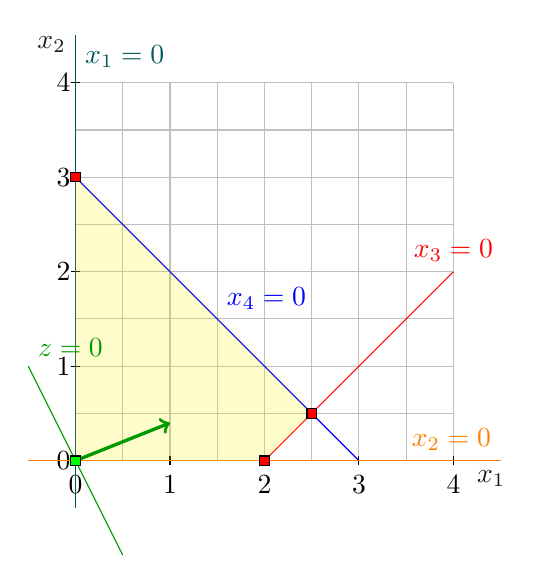
\begin{tikzpicture} [scale=1.2]
\draw[gray!50, thin, step=.5] (0,0) grid (4,4);
\draw[opacity=0.9] (0,0) -- (4.4,0) node[below] {$x_1$};
\draw[opacity=0.9] (0,0) -- (0,4.4) node[left] {$x_2$};

\foreach \x in {0,...,4} \draw (\x,0.05) -- (\x,-0.05) node[below] {\x};
\foreach \y in {0,...,4} \draw (-0.05,\y) -- (0.05,\y) node[left] {\y};

\draw [red](2, 0) --  (4, 2) node[above] {$x_3= 0$};
\draw [blue] (0,3)  -- node[above right] {$x_4=0$} (3,0) ;
\draw [teal!70!black](0,-.5) --  (0,4.5) node[below right] {$x_1=0$}; 
\draw [orange](-.5,0) --  (4.5,0) node[above left] {$x_2=0$}; 

\fill[yellow,opacity=0.2] (0,0) -- (2,0) -- (2.5,0.5) -- (0,3) -- cycle;

\draw [green!60!black] (-0.5, 1)  node[above right] {$z=0$} --  (0.5, -1)  ; % o.f.
\draw [green!60!black, very thick,->](0,0) -- (0+1, 0+2/5); % gradient

\filldraw[fill=green] (-0.05,-0.05) rectangle (0.05,0.05);
\filldraw[fill=red] (2.45,0.45) rectangle (2.55,0.55);
\filldraw[fill=red] (1.95,-0.05) rectangle (2.05,0.05);
\filldraw[fill=red] (-0.05,2.95) rectangle (0.05,3.05);    
\end{tikzpicture} \end{center} 
\end{minipage}

Luckily, this tableau already represents a basis, which has basic variables $\mathbf{x_B}=[x_3~x_4]^T$ (we can consider $z$ as a basic variable of sorts to complete the identity matrix).  Thus for this tableau we have $\mathbf{x_N}=[x_1~ x_2]^T$ ,
$\mathbf{B}$=$\left[ \begin{array}{rr} 1 & 0  \\  0 &  1 \\ \end{array} \right]$, 
$\mathbf{N}$=$\left[ \begin{array}{rr} 1 &-1  \\  1 &  1  \\ \end{array} \right]$.  This basic solution represents an extreme point if we set the nonbasic variables to zero, as we see in the graph of the LP in the nonbasic variable space. \\   

Here the basic variable values are $x_3 = 2$ and $x_4=3$, and $z = 0$. \\

The simplex algorithm (mostly), tableau version:
\begin{enumerate}
\item Put the LP into a standard form tableau, find a set of basic variables that form a feasible basis, and  modify the tableau to represent the basis using elementary row operations, we want the coefficients of the basic variables to form an identity matrix. 
\item Check optimality, for a maximization (minimization), if the Row~0 coefficients for the nonbasic variables are all nonnegative (nonpositive) then the basis is optimal. 
\item If the basis is not optimal, then find an adjacent basis that improves the solution. This will involve swapping one of the basic variables with a nonbasic variable to form a new basis. 
\item Select a nonbasic entering variable using Dantzig’s rule, specifically, for a maximization (minimization) problem pick the nonbasic variable with the smallest negative (largest positive) reduced cost. 
\item Select a variable to leave the basis.  Conceptually, as we increase the entering variable's value from zero, the values of the basis variables should change, the basic variable that goes to zero first is the leaving variable. To find the leaving variable, use the  ratio test.  For each row 1-$m$ having a positive coefficient in the entering variable column, divide the $rhs$ by the entering variable's (positive) coefficient. The basic variable corresponding to row with the smallest ratio is the leaving variable.  
\item Put the  tableau into the proper form for the new basis using elementary row operations and go to Step~2.
\end{enumerate}

\bigskip Consider the following example:

\begin{minipage}[t][][b]{.50\linewidth} \vspace{2mm}
\begin{center} \begin{tabular} {l|c||c|c|c|c|c|}  \cline{2-7}
max & $z$	& $x_1$ & $x_2$  & $x_3$	& $x_4$	& $rhs$ \\ \cline{2-7}
($z$)	    & 1		& -2        &  -1        &	 0 	    &	  0		&   0    \\ \cline{2-7}
($x_3$)			& 0		&	 1        &     -1     &	 1 			&	  0 		&	  2   \\
($x_4$)			& 0		&	  1       &	    1    &	 0 		&	  1 		&	   3   \\ \cline{2-7}
\end{tabular} \end{center}
\end{minipage}%
\begin{minipage}[t][][b]{.50\linewidth}
\begin{center}  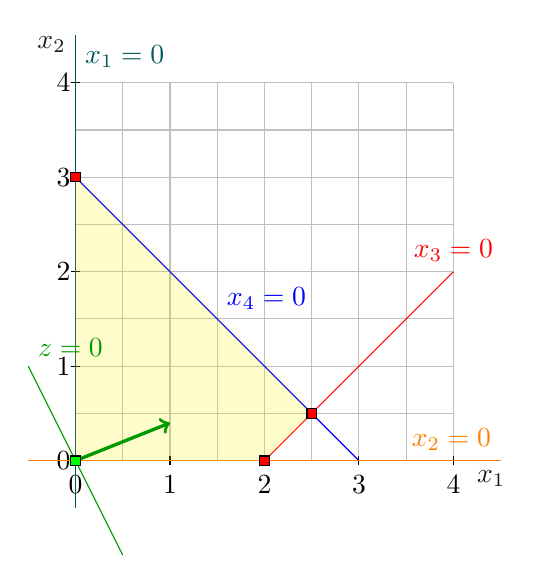
\begin{tikzpicture} [scale=1.2]
\draw[gray!50, thin, step=.5] (0,0) grid (4,4);
\draw[opacity=0.9] (0,0) -- (4.4,0) node[below] {$x_1$};
\draw[opacity=0.9] (0,0) -- (0,4.4) node[left] {$x_2$};

\foreach \x in {0,...,4} \draw (\x,0.05) -- (\x,-0.05) node[below] {\x};
\foreach \y in {0,...,4} \draw (-0.05,\y) -- (0.05,\y) node[left] {\y};

\draw [red](2, 0) --  (4, 2) node[above] {$x_3= 0$};
\draw [blue] (0,3)  -- node[above right] {$x_4=0$} (3,0) ;
\draw [teal!70!black](0,-.5) --  (0,4.5) node[below right] {$x_1=0$}; 
\draw [orange](-.5,0) --  (4.5,0) node[above left] {$x_2=0$}; 

\fill[yellow,opacity=0.2] (0,0) -- (2,0) -- (2.5,0.5) -- (0,3) -- cycle;

\draw [green!60!black] (-0.5, 1)  node[above right] {$z=0$} --  (0.5, -1)  ; % o.f.
\draw [green!60!black, very thick,->](0,0) -- (0+1, 0+2/5); % gradient

\filldraw[fill=green] (-0.05,-0.05) rectangle (0.05,0.05);
\filldraw[fill=red] (2.45,0.45) rectangle (2.55,0.55);
\filldraw[fill=red] (1.95,-0.05) rectangle (2.05,0.05);
\filldraw[fill=red] (-0.05,2.95) rectangle (0.05,3.05);    
\end{tikzpicture} \end{center} 
\end{minipage}

From the graph and tableau we can see that we are at the extreme point (0,0) and if we increase $x_1$ by one unit, the objective function ($z$-value) increases by 2, thus improving the solution.  We can increase $x_1$ by 2 and still remain in the feasible region, moving to extreme point (2,0).  Likewise, if we increase $x_2$ by one unit the objective function increases by 1, and we can increase $x_2$ by three and still remain in the feasible region, moving to extreme point (0,3).  As $x_2$ increases the basic variable $x_3$ gets larger, while the basic variable $x_4$ gets smaller, so $x_2$ enters the basis and $x_4$ leaves.\vspace{20mm}


\begin{minipage}[t][][b]{.50\linewidth} \vspace{2mm}
\begin{center} \begin{tabular} {l|c||c|c|c|c|c|}  \cline{2-7}
max 	& $z$	& $x_1$ & $x_2$  & $x_3$	& $x_4$	& $rhs$ \\ \cline{2-7}
$z$	    & 1		& 0     & -3     &	 2 	&	  0	&   4    \\ \cline{2-7}
$x_1$	& 0		& 1     & -1     &	 1 	&	  0 &	2   \\
$x_4$	& 0		& 0     &  2    &	-1 	&	  1 &	1   \\ \cline{2-7}
\end{tabular} \end{center}
\end{minipage}%
\begin{minipage}[t][][b]{.50\linewidth}
\begin{center}  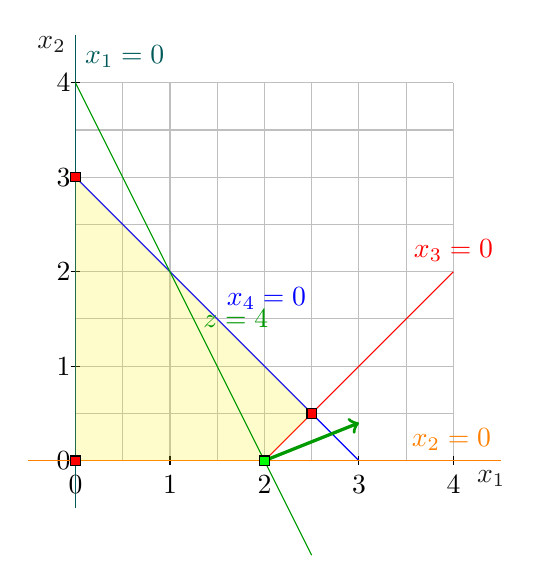
\begin{tikzpicture} [scale=1.2]
\draw[gray!50, thin, step=.5] (0,0) grid (4,4);
\draw[opacity=0.9] (0,0) -- (4.4,0) node[below] {$x_1$};
\draw[opacity=0.9] (0,0) -- (0,4.4) node[left] {$x_2$};

\foreach \x in {0,...,4} \draw (\x,0.05) -- (\x,-0.05) node[below] {\x};
\foreach \y in {0,...,4} \draw (-0.05,\y) -- (0.05,\y) node[left] {\y};

\draw [red](2, 0) --  (4, 2) node[above] {$x_3= 0$};
\draw [blue] (0,3)  -- node[above right] {$x_4=0$} (3,0) ;
\draw [teal!70!black](0,-.5) --  (0,4.5) node[below right] {$x_1=0$}; 
\draw [orange](-.5,0) --  (4.5,0) node[above left] {$x_2=0$}; 

\fill[yellow,opacity=0.2] (0,0) -- (2,0) -- (2.5,0.5) -- (0,3) -- cycle;

\draw [green!60!black] (0, 4)   -- node[right] {$z=4$}  (2.5, -1)  ; % o.f.
\draw [green!60!black, very thick,->](2,0) -- (2+1, 0+2/5); % gradient

\filldraw[fill=red] (-0.05,-0.05) rectangle (0.05,0.05);
\filldraw[fill=red] (2.45,0.45) rectangle (2.55,0.55);
\filldraw[fill=green] (1.95,-0.05) rectangle (2.05,0.05);
\filldraw[fill=red] (-0.05,2.95) rectangle (0.05,3.05);    
\end{tikzpicture} \end{center} 
\end{minipage}
~\vspace{30mm}

\begin{minipage}[t][][b]{.50\linewidth} \vspace{2mm}
\begin{center} \begin{tabular} {l|c||c|c|c|c|c|}  \cline{2-7}
max 	& $z$	& $x_1$ & $x_2$  & $x_3$	& $x_4$	& $rhs$ \\ \cline{2-7}
$z$	    & 1		& 0     & 0     &	 1/2 	&	3/2	&   11/2    \\ \cline{2-7}
$x_1$	& 0		& 1     & 0     &	 1/2 	&	 1/2 &	5/2    \\
$x_2$	& 0		& 0     & 1     &	-1/2 	&	 1/2&	1/2  \\ \cline{2-7}
\end{tabular} \end{center}
\end{minipage}%
\begin{minipage}[t][][b]{.50\linewidth}
\begin{center}  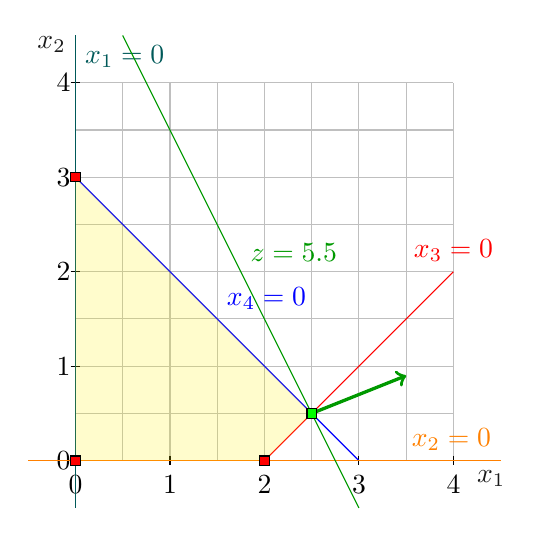
\begin{tikzpicture} [scale=1.2]
\draw[gray!50, thin, step=.5] (0,0) grid (4,4);
\draw[opacity=0.9] (0,0) -- (4.4,0) node[below] {$x_1$};
\draw[opacity=0.9] (0,0) -- (0,4.4) node[left] {$x_2$};

\foreach \x in {0,...,4} \draw (\x,0.05) -- (\x,-0.05) node[below] {\x};
\foreach \y in {0,...,4} \draw (-0.05,\y) -- (0.05,\y) node[left] {\y};

\draw [red](2, 0) --  (4, 2) node[above] {$x_3= 0$};
\draw [blue] (0,3)  -- node[above right] {$x_4=0$} (3,0) ;
\draw [teal!70!black](0,-.5) --  (0,4.5) node[below right] {$x_1=0$}; 
\draw [orange](-.5,0) --  (4.5,0) node[above left] {$x_2=0$}; 

\fill[yellow,opacity=0.2] (0,0) -- (2,0) -- (2.5,0.5) -- (0,3) -- cycle;

\draw [green!60!black] (0.5, 4.5)   -- node[above right] {$z=5.5$}  (3, -0.5)  ; % o.f.
\draw [green!60!black, very thick,->](2.5,0.5) -- (2.5+1, 0.5+2/5); % gradient

\filldraw[fill=red] (-0.05,-0.05) rectangle (0.05,0.05);
\filldraw[fill=green] (2.45,0.45) rectangle (2.55,0.55);
\filldraw[fill=red] (1.95,-0.05) rectangle (2.05,0.05);
\filldraw[fill=red] (-0.05,2.95) rectangle (0.05,3.05);    
\end{tikzpicture} \end{center} 
\end{minipage}

\vspace{10mm} Let's consider this algorithm, and what we know, and see if there are any missing parts, or other information we would find valuable.

\begin{itemize}
\item Unique optimal solution 
\item Multiple optimal solutions
\item Unbounded optimal objective value
\item Empty feasible region (an infeasible LP)
\end{itemize}

\vspace{10mm}{\bf Tableau Formulas:} \\

We can modify the tableau for a particular basis $\mathbf{B}$ using the following formulas:
\begin{center} \begin{tabular} {l|c|c|c|} \cline{2-4}
                    & $z$	        & $x_i$	                       &  $rhs$  \\ \cline{2-4}
 ($z$)         & 1	            & $\mathbf{c_BB^{-1}a_i -c_i}$ & $\mathbf{c_BB^{-1}b}$	    \\
 ($x_B$)  & $\mathbf{0}$	& $\mathbf{B^{-1}a_i}$	       & $\mathbf{B^{-1}b}$  \\ \cline{2-4}
\end{tabular} \end{center}
If we partition the variables, the formulas simplify as follows:
\begin{center} \begin{tabular} {l|c|c|c|c|} \cline{2-5}
       & $z$          & $x_{B}$	 & $x_{N}$                            & $rhs$ \\ \cline{2-5}
$z$    & 1	          & $\mathbf{c_BB^{-1}B-c_B=0}$ & $\mathbf{c_BB^{-1}N-c_{N}}$ & $\mathbf{c_BB^{-1}b}$ \\
$x_B$  & $\mathbf{0}$ & $\mathbf{B^{-1}B=I}$ & $\mathbf{B^{-1}N}$	       & $\mathbf{B^{-1}b}$ \\ \cline{2-5}
\end{tabular} \end{center} 

\bigskip The formulas for the coefficients for rows 1-$m$, that is $\mathbf{B^{-1}a_i}$ (or $\mathbf{B^{-1}A}$ for all the columns on the left-hand side) is fairly straight forward; Multiplying by $\mathbf{B^{-1}}$ is essentially the same as doing the elementary row operations required to get an identity matrix in the basic variable columns.  \\

Now consider the formula $\mathbf{c_BB^{-1}a_i -c_i}$ for the row~0 coefficients. Where did this come from? \\


Consider an expanded basis matrix $\mathbf{\hat{B}}$, which includes the $z$-variable column and row, as follows: $\left[ \begin{array}{cc}
    1 & -\mathbf{c_B} \\
    0 & \mathbf{B} \\
\end{array} \right],$
which yields $\mathbf{\hat{B}^{-1}}$ of $\left[ \begin{array}{cc}
    1 & \mathbf{c_BB^{-1}} \\
    0 & \mathbf{B^{-1}} \\
\end{array} \right],$
and the column for $x_i$ is $[-c_i, \mathbf{a_i}]^T$.  Multiplying these yields $\left[
\begin{array}{cc}
 1         & \mathbf{c_BB^{-1}} \\
\mathbf{0} & \mathbf{B^{-1}} \\
\end{array} \right] \left[
\begin{array}{c}
     -c_i \\
     \mathbf{a_i} \\
\end{array} \right],$
which results in dot product of  $[1,\mathbf{c_BB^{-1}}][-c_i, \mathbf{a_i}] = \mathbf{c_BB^{-1}a_i} - c_i$ for the first element of the resulting column vector. \\

\vspace{5mm} For example, consider the following LP:
\begin{align*}
\mbox{Max~~} & z = 2x_1 + 3x_2  \\
\mbox{s.t.~~}  & 1x_1 + 1x_2 \ge 2 \\
&      4x_1 + 6x_2 \le 9 \\
&      x_1, x_2 \ge 0. 
\end{align*}

For this problem, if we have $x_1$ ad $x_2$ as the basic variables, then \\

$\mathbf{\hat{B}} = \left[ \begin{array}{ccc}
    1 & -2 & -3 \\
    0 &  1 &  1 \\
    0 &  4 &  6 \\
\end{array} \right]$
and $\mathbf{\hat{B}^{-1}} = \left[ \begin{array}{ccc}
    1 &  0  & 1/2   \\
    0 &  3  &  -1/2 \\
    0 &  -2 &  1/2 \\
\end{array} \right],$ \\

and the column for $x_1$ is $[-2, 1, 4]^T$.  \\

When we multiply $\mathbf{\hat{B}^{-1}}$ and $[-2, 1, 4]^T$ we get \\

$\left[\begin{array}{ccccccc}
    1 & 0  & 1/2    &~& -2  & & 0 \\
    0 & 3  & -1/2   &~& 1   &=& 1 \\
    0 & -2 &  1/2   &~& 4   & & 0 \\
\end{array} \right]$


\vspace{10mm}The simplex algorithm again:
\begin{enumerate}
\item Put the LP into a standard form tableau, find a feasible basis $\mathbf{B}$ and  modify the tableau using  $\mathbf{B^{-1}}$ and the tableau formulas.
\item Check optimality, if $\mathbf{c_BB^{-1}a_i -c_i} \ge (\le)~0$ for $i: x_i \in \mathbf{x_N}$ for a maximization (minimization) problem, then the current basic solution is optimal. Stop.
\item Select an entering nonbasic variable using Dantzig's rule, specifically, entering variable $x_i$, where $i =$ \\
$ \text{min (max)}_i~\{ \mathbf{c_BB^{-1}a_i -c_i} < (>)~ 0: (i: x_i \in \mathbf{x_N})\}$ for a maximization (minimization) problem.
\item Select a variable to leave the basis using the ratio test. For entering variable $x_i$ the leaving variable is the basic variable corresponding to row~$j$, where :\\
$\text{min}_j \{[\mathbf{B^{-1}b}]_j/[\mathbf{B}^{-1}\mathbf{a_i}]_j,~( j:j = 1, \cdots,m,~[\mathbf{B}^{-1}\mathbf{a_i}]_j > 0)\}$.
\item Put the  tableau into the proper form for the new basis and go to Step~2.
\end{enumerate}



\underline{\bf Finding an Initial BFS}
When a basic feasible solution is not apparent, we an produce one using {\it artificial variables}.  This {\it artificial} basis is undesirable from the perspective of the original problem, we do not want the artificial variables in our solution, so we penalize them in the objective function, and allow the simplex algorithm to drive them to zero (if possible) and out of the basis.  There are two such methods, the {\bf Big M method} and the {\bf Two-phase method}, which we illustrate below:

\vspace{10mm}  Solve the following LP using the Big M Method and the simplex algorithm:

\begin{align*}
max~~ & z = 9x_1 + 6x_2 \\
s.t.~~
&  3x_1 + 3x_2 \le 9 \\
&  2x_1 - 2x_2 \ge 3 \\
&  2x_1 + 2x_2 \ge 4 \\
& x_1, x_2 \ge 0. \\
\end{align*}

Here is the LP is transformed into standard form by using slack variables $x_3$, $x_4$, and $x_5$, with the required artificial variables $x_6$ and $x_7$, which allow us to easily find an initial basic feasible solution (to the artificial problem).
\begin{eqnarray}
& max  & z_a = 9x_1 + 6x_2 -M x_6 - M x_7 \nonumber \\
& s.t. & 3x_1 + 3x_2 + x_3 = 9 \nonumber \\
&      & 2x_1 - 2x_2 - x_4 + x_6 = 3 \nonumber \\
&      & 2x_1 + 2x_2 - x_5 + x_7 = 4 \nonumber \\
&      & x_i \ge 0,~~ i =1,\cdots,7. \nonumber
\end{eqnarray}

\begin{center} \begin{tabular} {|c|c|c|c|c|c|c|c||c| r} \cline{1-9}
$z$	& $x_1$	& $x_2$	& $x_3$	& $x_4$	& $x_5$	& $x_6$	& $x_7$	& RHS &	ratio \\ \cline{1-9}
1	&	 -9 &	 -6 &	 0 &	  0 &	  0 &	  M &	  M &	0 & \\
0	&	  3 &	  3 &	 1 &	  0 &	  0 &	  0 &	  0 &	9 &	 \\
0	&	  2 &	 -2 &	 0 &	 -1 &	  0 &	  1 &	  0 &	3 & \\
0	&	  2 &	  2 &	 0 &	  0 &	 -1 &	  0 &	  1 &	4 &	 \\
\cline{1-9}
\end{tabular} \end{center}
\noindent This tableau is not in the correct form, it does not represent a basis, the columns for the artificial variables need to be adjusted.

\begin{center} \begin{tabular} {|c|c|c|c|c|c|c|c||c| r} \cline{1-9}
$z$	& $x_1$	  & $x_2$  & $x_3$	& $x_4$	& $x_5$	& $x_6$	& $x_7$	& RHS &	ratio \\ \cline{1-9}
1	& -9 - 4M & -6     &	 0 &	  M &	  M &	  0 &	  0 & -7M &	      \\
0	&	  3   &	     3 &	 1 &	  0 &	  0 &	  0 &	  0 &	9 &	3     \\
0	&	  2   &	    -2 &	 0 &	 -1 &	  0 &	  1 &	  0 &	3 &	3/2   \\
0	&	  2   &	     2 &	 0 &	  0 &	 -1 &	  0 &	  1 &	4 &	2     \\
\cline{1-9}
\end{tabular} \end{center}
\noindent The current solution is not optimal, so $x_1$ enters the basis, and by the ratio test, $x_6$ (an artificial variable) leaves the basis.

\begin{center} \begin{tabular} {|c|c|c|c|c|c|c|c||c| r} \cline{1-9}
$z$	&   $x_1$ & $x_2$   & $x_3$	& $x_4$	& $x_5$	& $x_6$	   & $x_7$	& RHS      & ratio \\
\cline{1-9}
1	&     0   & -15 -4M &	 0 & -9/2 -M &	  M & 9/2 + 2M &	  0 &  27/2 -M &    	\\
0	&	  0   &	     6  &	 1 &	 3/2 &	  0 &	    -3/2 &	  0 &	3/2    & 3/4     \\
0	&	  1   &	    -1  &	 0 &	-1/2 &	  0 &	   1/2 &	  0 &	3/2    & -  	\\
0	&	  0   &	     4  &	 0 &	   1 &	 -1 &	     -1 &	  1 &	  1    & 1/4        	\\ \cline{1-9}
\end{tabular} \end{center}
\noindent The current solution is not optimal, so $x_2$ enters the basis, and by the ratio test, $x_7$ (an artificial variable) leaves the basis.

\begin{center} \begin{tabular} {|c|c|c|c|c|c|c|c||c|r} \cline{1-9}
$z$	&   $x_1$ & $x_2$ & $x_3$ & $x_4$	& $x_5$	& $x_6$	   & $x_7$	& RHS     &	ratio \\
\cline{1-9}
1	&     0   &     0 &	 0    & -3/4    & -15/4 &        - &	  - &  17 1/4 &	   \\
0	&	  0   &	    0 &	 1    &	   0    &	3/2 &	     0 &   -3/2 &	  3   &	-  \\
0	&	  1   &	    0 &	 0    &	-1/4    &  -1/4 &	   1/2 &	1/4 &	  7/4 &	-  	\\
0	&	  0   &	    1 &	 0    &	 1/4    &  -1/4 &	  -1/4 &	1/4 &	  1/4 & 1   \\
\cline{1-9}
\end{tabular} \end{center}
\noindent The current solution is not optimal, so $x_4$ enters the basis, and by the ratio test, $x_2$ leaves the basis.

\begin{center} \begin{tabular} {|c|c|c|c|c|c|c|c||c|r} \cline{1-9}
$z$	&   $x_1$ & $x_2$ & $x_3$ & $x_4$ & $x_5$ & $x_6$ & $x_7$ & RHS     &	ratio \\
\cline{1-9}
1	&     0   &    3  &	 0    & 0     & -9/2  &     - &	    - &  18 &	   \\
0	&	  0   &	    0 &	 1    &	   0  &	  3/2 &	    0 &  -3/2 &	  3     &	-  \\
0	&	  1   &	    1 &	 0    &	0     &  -1/2 &	   0  &	  1/2 &	  2   &	-  	\\
0	&	  0   &	    4 &	 0    &	 1    &  -1   &	  -1 &      1 &	  1    & 1   \\ \cline{1-9}
\end{tabular} \end{center}
\noindent The current solution is not optimal, so $x_5$ enters the basis, and by the ratio test, $x_3$ leaves the basis.

\begin{center} \begin{tabular} {|c|c|c|c|c|c|c|c||c|r} \cline{1-9}
$z$	&   $x_1$ & $x_2$ & $x_3$ & $x_4$ & $x_5$ & $x_6$ & $x_7$ & RHS     &	ratio \\
\cline{1-9}
1	&     0   &    3  &	 3    & 0     & 0  &     - &	    - &  27 &	   \\
0	&	  0   &	    0 &	 2/3  &	  0   &	  1 &	    0 &  -1 &	  2     &	 \\
0	&	  1   &	    1 &	 1/3   &   0  &  0 &	   0  &	  0 &	  3   &  	\\
0	&	  0   &	    4 &	 2/3   &	1 &  0   &	  -1 &     0&	 3    &    \\
\cline{1-9}
\end{tabular} \end{center}
The current solution is optimal! \\

\bigskip Solve the following LP using the Two-phase Method and Simplex Algorithm.
\begin{align*}
max~~ & z = 2x_1 + 3x_2   \\
s.t.~~ 
& 3x_1 + 3x_2 \ge 6  \\
& 2x_1 - 2x_2 \le 2  \\
& -3x_1 + 3x_2 \le 6   \\
& x_1, x_2 \ge 0. 
\end{align*}


%\begin{center} \includegraphics[scale=0.7]{Figs_N/TwoPhase}\end{center}

Here is first phase LP (in standard form), where $x_3$, $x_4$, and $x_5$ are slack variables, and $x_6$ is an artificial variable.
\begin{eqnarray}
& min  & z_a = x_6 \nonumber \\
& s.t. & 3x_1 + 3x_2 - x_3 +x_6 = 6 \nonumber \\
&      & 2x_1 - 2x_2 + x_4 = 2 \nonumber \\
&      & -3x_1 + 3x_2 + x_5 = 6 \nonumber \\
&      & x_i \ge 0,~~ i =1,\cdots,6. \nonumber
\end{eqnarray}
Next, we put the LP into a tableau, which, still is not in the right form for our basic variables ($x_6$, $x_4$, and $x_5$).
\begin{center} \begin{tabular} {|c|c|c|c|c|c|c||c| r} \cline{1-8}
$z$	& $x_1$	& $x_2$	& $x_3$	& $x_4$	& $x_5$	& $x_6$	&  RHS & ratio \\ \cline{1-8}
1	&	  0 &	  0 &	 0 &	  0 &	  0 &	 -1 &    0 & \\
0	&	  3 &	  3 &	-1 &	  0 &	  0 &	  1 &	 6 & \\
0	&	  2 &	 -2 &	 0 &	  1 &	  0 &	  0 &	 2 & \\
0	&	  -3 &	  3 &	 0 &	  0 &	  1 &	  0 &	 6 & \\ \cline{1-8}
\end{tabular} \end{center}
To remedy this, we use row operation to modify the row 0 coefficients, yielding the following:
\begin{center} \begin{tabular} {|c|c|c|c|c|c|c||c| r} \cline{1-8}
$z$	& $x_1$	& $x_2$	& $x_3$	& $x_4$	& $x_5$	& $x_6$	&  RHS & ratio \\ \cline{1-8}
1	&	  3 &	  3 &	 -1 &	  0 &	  0 &	  0 &    6 &   \\
0	&	  3 &	  3 &	-1 &	  0 &	  0 &	  1 &	 6 &  2 \\
0	&	  2 &	 -2 &	 0 &	  1 &	  0 &	  0 &	 2 &  - \\
0	&	  -3 &	  3 &	 0 &	  0 &	  1 &	  0 &	 6 &  2 \\ \cline{1-8}
\end{tabular} \end{center}
The current solution is not optimal, either $x_1$ or $x_2$ can enter the basis, let's choose $x_2$. Then by the ratio test, either $x_6$ (an artificial variable) or $x_5$ (a slack variable) can leaves the basis.  Let's choose $x_6$.
\begin{center} \begin{tabular} {|c|c|c|c|c|c|c||c| r} \cline{1-8}
$z$	& $x_1$	& $x_2$	& $x_3$	& $x_4$	& $x_5$	& $x_6$	&  RHS & ratio \\ \cline{1-8}
1	&	  0 &	  0 &	 0 &	  0 &	  0 &  -1 &    0 & \\
0	&	  1 &	  1 &	-1/3 &	  0 &	  0 &   1/3 &	 2 & \\
0	&	  4 &	  0 &	-2/3 &	  1 &	  0 &   2/3 &	 6 & \\
0	&	 -6 &	  0 &	 1 &	  0 &	  1 &	 -1 &	 0 & \\ \cline{1-8}
\end{tabular} \end{center}
The current solution is optimal, so we end the first phase with a basic feasible solution to the original problem, with $x_2$, $x_4$, and $x_5$ as the basic variables.  Now we provide a new row zero that corresponds to the original problem.

\begin{center} \begin{tabular} {|c|c|c|c|c|c|c||c| r} \cline{1-8}
$z$	& $x_1$	& $x_2$	& $x_3$	& $x_4$	& $x_5$	& $x_6$	&  RHS & ratio \\ \cline{1-8}
1	&	  1 &	  0 &	 -1 &	  0 &	  0 &	  0 &   6 & \\
0	&	  1 &	  1 &	-1/3 &	  0 &	  0 &	  1/3 &	 2 &   \\
0	&	  4 &	  0 &	-2/3 &	  1 &	  0 &	  2/3 &	 6 &  \\
0	&	 -6 &	  0 &	 1 &	  0 &	  1 &	  -1 &	 0 &  \\ \cline{1-8}
\end{tabular} \end{center}

\begin{center} \begin{tabular} {|c|c|c|c|c|c|c||c| r} \cline{1-8}
$z$	& $x_1$	& $x_2$	& $x_3$	& $x_4$	& $x_5$	& $x_6$	&  RHS & ratio \\ \cline{1-8}
1	&	 -5 &	  0 &	  0 &	  0 &	  1 &	  -1 &   6 & \\
0	&	 -1 &	  1 &	  0 &	  0 &	1/3 &	  0 &	 2 &   \\
0	&	  0 &	  0 &	  0 &	  1 &	2/3 &	  0 &	 6 &  \\
0	&	 -6 &	  0 &	  1 &	  0 &	  1 &	  -1 &	 0 &  \\ \cline{1-8}
\end{tabular} \end{center}
From this tableau we can see that the LP is unbounded and an extreme point is [0, 2, 0, 6,0] and an extreme direction is [1, 1, 6, 0, 0].




\underline{\bf Degeneracy and the Simplex Algorithm}
\begin{comment}
$\mathbf {n} \cdot (\mathbf {r} -\mathbf {r} _{0})=0.$
(The dot here means a dot (scalar) product.) Expanded this becomes

$a(x-x_{0})+b(y-y_{0})+c(z-z_{0})=0$
which is the point-normal form of the equation of a plane.  This is just a linear equation

$ax+by+cz+d=0$,
where

$d=-(ax_{0}+by_{0}+cz_{0}).$  
Conversely, it is easily shown that if a, b, c and d are constants and a, b, and c are not all zero, then the graph of the equation

$ax+by+cz+d=0$ is a plane having the vector 

$\mathbf{ n} = (a, b, c)$ as a normal. 

This plane can also be described by the "point and a normal vector" prescription above. A suitable normal vector is given by the cross product
${\mathbf {n}}=({\mathbf {p}}_{2}-{\mathbf {p}}_{1})\times ({\mathbf {p}}_{3}-{\mathbf {p}}_{1})$,

and the point r0 can be taken to be any of the given points p1,p2 or p3[6] (or any other point in the plane).
Let p1=(x1, y1, z1), p2=(x2, y2, z2), and p3=(x3, y3, z3) be non-collinear points.

${\displaystyle \mathbf {w\times v} ={\begin{vmatrix}\mathbf {i} &\mathbf {j} &\mathbf {k} \\w_{1}&w_{2}&w_{3}\\v_{1}&v_{2}&v_{3}\\\end{vmatrix}}}$

${\displaystyle {\begin{aligned}\mathbf {w\times v} &={\begin{vmatrix}w_{2}&w_{3}\\v_{2}&v_{3}\end{vmatrix}}\mathbf {i} -{\begin{vmatrix}w_{1}&w_{3}\\v_{1}&v_{3}\end{vmatrix}}\mathbf {j} +{\begin{vmatrix}w_{1}&w_{2}\\v_{1}&v_{2}\end{vmatrix}}\mathbf {k} \\&=(w_{2}v_{3}-w_{3}v_{2})\mathbf {i} +(w_{3}v_{1}-w_{1}v_{3})\mathbf {j} +(w_{1}v_{2}-w_{2}v_{1})\mathbf {k} ,\end{aligned}}}$
\end{comment}

Degeneracy must be considered in the simplex algorithm, as it causes some trouble.  For instance, it might mislead us into thinking there are multiple optimal solutions, or provide faulty insight.  Further, the algorithm as described can {\it cycle}, that is, remain on a degenerate extreme point repeatedly cycling through a subset of bases that represent that point, never leaving. 

\begin{center} \begin{tabular} {c|c|c|c|c|c|c|c|c|c|} \cline{2-10}
min &$z$	& $x_1$ & $x_2$ & $x_3$	& $x_4$	&  $x_5 $& $x_6$ & $x_7$ & $rhs$ \\ \cline{2-10}
       &1		& 0 		  & 0         &	 0 	    &	  3/4     &   -20 & 1/2 & -6  &     0    \\ \cline{2-10}
       &0		&	 1       &	    0   &	 0 			&	  1/4 		&	-8 & -1 &   9 &   0	  \\
       &0		&	 0     &	    1      &	 0 		&	  1 /2		&	 -12 & -1/2 & 3 & 0   \\ 
       &0		&	 0     &	    0      &	 1 		&	  0		&	 0 & 1 & 0 &1   \\ \cline{2-10}
\end{tabular} \end{center}


\bigskip  Solve the following LP using the Simplex Algorithm:
\begin{eqnarray}
& \max  & z = 40x_1 + 30x_2 \nonumber \\
& s.t. & 6x_1 + 4x_2 \le 40 \nonumber \\
&      & 4x_1 + 2x_2 \le 20 \nonumber \\
&      & x_1, x_2 \ge 0. \nonumber
\end{eqnarray}

By adding slack variables, we have the following tableau.
\begin{table}[h!] \begin{center} \begin{tabular} {|c|c|c|c|c||c|}
\hline
$z$ & $x_1$ & $x_2$ & $s_1$ & $s_2$ & RHS \\ \hline
  1 & -40 & -30 & 0   & 0   & 0  \\
  0 &   6 &   4 & 1   & 0   & 40 \\
  0 &   4 &   2 & 0   & 1   & 20 \\ \hline
\end{tabular} \end{center} \end{table}
Luckily, this tableau represents a basis, where BV=$\{s_1, s_2\}$, but by inspecting the row 0 (objective function row) coefficients, we can see that this is not optimal. By Dantzig's Rule, we enter $x_1$ into the basis, and by the ratio test we see that $s_2$ leaves the basis.  By performing elementary row operations, we obtain the following tableau for
the new basis BV=$\{s_1, x_1\}$.
\begin{center} \begin{tabular} {|c|c|c|c|c||c|} \hline
$z$ & $x_1$ & $x_2$ & $s_1$ & $s_2$ & RHS \\
\hline
  1 &     0 &   -10 & 0     &    10 & 200 \\
  0 &     0 &     1 & 1     &  -3/2 & 10 \\
  0 &     1 &   1/2 & 0     &   1/4 &  5 \\
\hline
\end{tabular} \end{center}

This tableau is not optimal, entering $x_2$ into the basis can improve the objective function value. The basic variables $s_1$ and $x_1$ tie in the ration test.  If we have $x_1$ leave the basis, we get the following tableau (BV=$\{s_1, x_2\}$).
\begin{center} \begin{tabular} {|c|c|c|c|c||c|}
\hline
$z$ & $x_1$ & $x_2$ & $s_1$ & $s_2$ & RHS \\
\hline
  1 &    20 &     0 &     0 &    15 & 300 \\
  0 &    -2 &     0 &     1 &    -2 &  0 \\
  0 &     2 &     1 &     0 &   1/2 &  10 \\ \hline
\end{tabular} \end{center}
This is an optimal tableau, with an objective function value of 300,  If instead of $x_1$ leaving the basis, suppose $s_1$ left, this would lead to the following tableau (BV=$\{x_2, x_1\}$).
\begin{center} \begin{tabular} {|c|c|c|c|c||c|} \hline
$z$ & $x_1$ & $x_2$ & $s_1$ & $s_2$ & RHS \\
\hline
  1 &     0 &     0 &    10 &    -5 & 300 \\
  0 &     0 &     1 &     1 &  -3/2 &  10 \\
  0 &     1 &     0 &  -1/2 &     1 &   0 \\ \hline
\end{tabular} \end{center}
This tableau does not look optimal, yet the objective function value is the same as the optimal solution's. This occurs because the optimal extreme point is a degenerate.% as the following figure shows.


%\begin{center} \includegraphics[scale=0.7]{Figs_N/degen} \end{center}

\subsubsection{Dual Simplex Algorithm}
The dual simplex algorithm is essentially performing the simplex algorithm, on the dual problem, on the primal tableau. Remember, the Simplex algorithm, in relation to the KKT conditions, maintains primal feasibility, complementary slackness, and strives for dual feasibility. The dual simplex algorithm maintains dual feasibility, complementary slackness, and strives for primal feasibility. \\

\begin{enumerate}
\item Pick the row with the smallest $\bar{b}_i$, where $\bar{b}_i < 0$ ($\mathbf{\bar{b}} = \mathbf{B^{-1}b}$), this corresponds to the leaving variable.
\item Pick a column with the minimum $\{|z_j -c_j/y_{ij}|:y_{ij} < 0\}$, this corresponds to the entering variable.
\item Pivot, and repeat until primal feasibility is achieved.
\end{enumerate}



\subsubsection{Primal-Dual Algorithm}
The primal dual algorithm is another method for solving LPs. This algorithm starts with a feasible dual solution (not necessarily basic) and searches for a primal feasible solution will maintaining complementary slackness between the primal and dual solutions.  Consider the following primal dual pair:

\begin{align*}
&(P):\min\{\mathbf{cx}: \mathbf{Ax} = \mathbf{b}, \mathbf{x} \ge 0\} \\
&(D):\max\{{\bf wb}: \mathbf{wA} \le \mathbf{c}, {\bf w}~urs\}.
\end{align*}
To solve $P$ using the primal-dual algorithm, first find a feasible solution to $D$, it does not necessarily have to be basic, and form the following restricted primal problem:
$$(P_R):\min\{z_R= {\bf 1x^a}: \mathbf{a_j}x_j+\mathbf{x^a\mathbf} = \mathbf{b}, x_j \ge 0,~ j \in Q,~\mathbf{x^a} \ge \mathbf{0}\},$$
where $Q=\{j:wa_j = c_j\}$, that is, $Q$ is the set of indexes for binding dual constraints, and $x_j, j \in Q$ are the primal variables that can be non-zero given the current dual solution and complementary slackness. The vector $\mathbf{x^a}$ is a vector of artificial variables; this problem looks very similar to the phase~1 problem in the two-phase method.  The objective is the same, to find a basic feasible primal solution, but here we use a {\it restricted} or limited number of primal variables, those with indexes in set $Q$.\\

Solve $P_R$ (using simplex) and if $z_R=0$, stop, the solution is optimal for $P$ because we have satisfied the KKT conditions, else let $\mathbf(v)^*$ be the corresponding optimal dual solution $D_R$.

$$D_R:\max\{\mathbf{vb}: \mathbf{va_j }\le 0,~ i \in Q, \mathbf{v} \le 1, \mathbf{v}~ urs\}.$$

Note that for each $j \in Q$, $\mathbf{v^*a_j} \le 0$. For $i \notin Q$ calculate $\mathbf{v^*a_i}$, if $\mathbf{v^*a_i} > 0$ then $x_i$ can be added to the restricted primal to improve $z_R$.  To get $x_i$ into $Q$ we must modify the original dual solution $\mathbf{w}$, first we calculate $\theta$.

$$ \theta = \min_{i \notin Q} \{|(\mathbf{wa_i}-c_i)|/\mathbf{v^*a_i} : \mathbf{v^*a_i} > 0\}  > 0$$ 

We take the absolute value of $\mathbf{wa_i}-c_i)$ because if the primal problem is a minimization, this term will always be non-positive, for a primal maximization this will always be non-negative (thus the absolute value is not needed). \\

We then replace $\mathbf{w}$ by $\mathbf{w}+\theta\mathbf{v^*}$.  We use this $\theta$-step like a ratio test, changing the current dual solution such that we can enter a new primal variable into the restricted primal, one that will improve the solution (and move us closer to feasibility), while maintaining dual feasibility and complementary slackness.  \\

If we think about this algorithm on a tableau, we get the following formulas, where the $z_P$ row corresponds to our dual solution, and defines the set $Q$, and simplex is performed on on the restricted problem (using row $z^R_P$ for the objective function row, and using column defined by $Q$). 

\begin{center} \begin{tabular} {c|c|c|c|c|c|} \cline{2-6}       
		& $z$ 	& $\mathbf{x}$ 			& $\mathbf{x^s}$ 		& $\mathbf{x^a}$	& rhs  \\ \cline{2-6}\cline{2-6} 
$z_P$  	& 1  	& $\mathbf{wa_i}-c_i$	& $\mathbf{wa_i}$		& 0					& 0    \\ \cline{2-6}
$z^R_P$ & 1		& $\mathbf{va_i} $   	& $\mathbf{va_i} $		& $\mathbf{va_i}-1$ & 0    \\ \cline{2-6} \cline{2-6}       
		& 0     & $\mathbf{B^{-1}a_i}$	& $\mathbf{B^{-1}a_i}$& $\mathbf{B^{-1}a_i}$ 	& $\mathbf{B^{-1}b}$   \\ \cline{2-6}
\end{tabular} \end{center}


\begin{example}{Primal-dual algorithm}{primal-dual-alg}
Consider again the following LP and solve using the primal-dual algorithm, using a starting feasible dual solution of $\mathbf{w} = [10,0,0]$.
\end{example}
\begin{solution}

\begin{eqnarray}
& \max  & 18x_1 + 16x_2 + 10x_3  \nonumber \\
& s.t. & 2x_1 + 2x_2 + 1x_3 +x^s_4 = 21~~ (w_1) \nonumber \\
&      & 3x_1 + 2x_2 + 2x_3 + x^s_5 = 23~~ (w_2) \nonumber \\
&      & 1x_1 + 2x_2 + 1x_3 +x_6 = 17~~ (w_3) \nonumber \\
&      & x_1, x_2, x_3, x_4, x_5, x_6 \ge 0. \nonumber
\end{eqnarray}
\begin{eqnarray}
D1:& \min  & 21w_1 +23w_2 +17w_3  \nonumber \\
   & s.t. & 2w_1 +3w_2 + 1w_3 \ge 18~~ (x_1) \nonumber \\
   &      & 2w_1 +2w_2 + 2w_3 \ge 16~~ (x_2) \nonumber \\
   &      & 1w_1 +2w_2 + 1w_3 \ge 10~~ (x_3) \nonumber \\
   &      & w_1, w_2, w_3 \ge 0. \nonumber
\end{eqnarray}
Use the modified tableau method, and write $Q$ and the restricted problem for each step.  Be able to explain the complete process.

For $\mathbf{w} = [10,0,0]$ we have $Q=\{3,5,6\}$
\begin{center} \begin{tabular} {|c|c|c|c|c|c|c|c|c|}
\hline       & $x_1$ & $x_2$ & $x_3$ & $x^s_4$ & $x^s_5$ & $x^s_6$ &$x^a_7$ & rhs   \\ \hline
\hline $z$   & 2     & 4     & 0      & 10   & 0     & 0     &  0    & 210   \\
\hline $z_R$ & 0     & 0     & 0      & 0    & 0     & 0     & -1    & 0     \\
\hline       & 2     & 2     & 1      & 1    & 0     & 0     & 1     & 21    \\
\hline       & 3     & 2     & 2      & 0    & 1     & 0     & 0     & 23   \\
\hline       & 1     & 2     & 1      & 0    & 0     & 1     & 0     & 17   \\ \hline
\end{tabular} \end{center} \label{T1}

We need to make a minor adjustment to the artificial variable column.
\begin{center} \begin{tabular} {|c|c|c|c|c|c|c|c|c|c|} \hline       
			& $z_P$ & $x_1$ & $x_2$ & $x_3$ & $x^s_4$ 	& $x^s_5$ 	& $x^s_6$ 	& $x^a_7$ 	& rhs  \\ \hline\hline 
$z_P$ 	&  1  	& 2    	& 4     & 0     & 10   		& 0     	& 0  & 0   & 210   \\ \hline 
$z_R$ 	&  1	& 2    	& 2     & \hi 1     & 1    		& \hi 0     	&\hi 0     	&\hi 0     	&\hi 21    \\ \hline \hline       
			&  0    & 2     & 2     & \hi 1     & 1    		& \hi 0     	& \hi 0     	&\hi 1 &\hi  21    \\ \hline       
		& 0 	& 3     & 2     & \hi 2     & 0    		& \hi 1     	&\hi 0     	&\hi 0     	&\hi 23   \\ \hline       
		& 0 	& 1     & 2     & \hi 1      & 0    	&\hi  0     	&\hi 1     	&\hi 0     	&\hi 17   \\ \hline
\end{tabular} \end{center}

$x_3$ enters the restricted basis and $x^s_5$ leaves the restricted basis, resulting in the following tableau:
\begin{center} \begin{tabular} {|c|c|c|c|c|c|c|c|c|} \hline      
         & $x_1$ & $x_2$ & $x_3$  & $x^s_4$ 	& $x^s_5$ 	& $x^s_6$ & $x^a_7$ & rhs  \\ \hline \hline 
$z$   & 2     & 4     & 0      & 10   & 0     & 0     & 0     & 210   \\ \hline 
$z_R$ & 1/2   & 1     &\hi 0      & 1     &\hi -1/2  &\hi 0     &\hi 0      &\hi 19/2   \\ \hline \hline
       & 1/2   & 1     &\hi 0      & 1     &\hi -1/2  &\hi0     &\hi 1      &\hi 19/2   \\ \hline 
      & 3/2   & 1     &\hi 1      & 0     &\hi 1/2   &\hi 0     &\hi 0      &\hi 23/2   \\ \hline 
      & -1/2  & 1     &\hi 0      & 0     &\hi -1/2  &\hi 1     &\hi 0      &\hi 11/2   \\ \hline
\end{tabular} \end{center}

To find $\Theta$ we take the minimum of 4/1 and 2/(1/2), which are equal, and thus $\Theta=4$, using this we adjust the $z$-row, yielding the following tableau. Notice that this operation ensures that the $z$-row remains non-negative. Now $Q=\{1,2,3,6\}$. 

\begin{center} \begin{tabular} {|c|c|c|c|c|c|c|c|c|} \hline      
         & $x_1$ & $x_2$ & $x_3$  & $x^s_4$ 	& $x^s_5$ 	& $x^s_6$ & $x^a_7$ & rhs  \\ \hline \hline 
$z$   & 0     & 0     & 0      & 6   & 2     & 0     & 0     & 172   \\ \hline 
$z_R$ &\hi 1/2   &\hi 1     &\hi 0      & 1     & -1/2  &\hi 0     &\hi 0      &\hi 19/2   \\ \hline \hline
       &\hi 1/2   &\hi 1     &\hi 0      & 1     & -1/2  &\hi0     &\hi 1      &\hi 19/2   \\ \hline 
      &\hi 3/2   &\hi1     &\hi 1      & 0     & 1/2   &\hi 0     &\hi 0      &\hi 23/2   \\ \hline 
      &\hi -1/2  &\hi 1     &\hi 0      & 0     & -1/2  &\hi 1     &\hi 0      &\hi 11/2   \\ \hline
\end{tabular} \end{center}
$x_2$ enters the basis (of the restricted problem) and $x_6$ leaves.
\begin{center} \begin{tabular} {|c|c|c|c|c|c|c|c|c|}
\hline       & $x_1$ & $x_2$ & $x_3$  & $x^s_4$ 	& $x^s_5$ 	& $x^s_6$ & $x^a_7$ & rhs  \\ \hline \hline
$z$    	& 0     & 0     & 0      & 6     & 2     & 0     & 0      & 172 \\ \hline
$z_R$ 	&\hi 1     &\hi 0     &\hi 0      & 1     & 0     &\hi -1    &\hi 0      &\hi 4   \\ \hline \hline
      &\hi 1     &\hi 0     &\hi 0      & 1     & 0     & \hi-1    &\hi 1      &\hi 4   \\ \hline 
      &\hi 2     &\hi 0     &\hi 1      & 0     & 1     &\hi -1    &\hi 0      &\hi 6   \\ \hline 
       &\hi -1/2  &\hi 1     &\hi 0      & 0     & -1/2  &\hi 1     &\hi 0      &\hi 11/2   \\ \hline
\end{tabular} \end{center}

This is not an optimal solution, so now $x_1$ enters the restricted basis and $x_3$ leaves.
\begin{center} \begin{tabular} {|c|c|c|c|c|c|c|c|c|}
\hline       & $x_1$ & $x_2$ & $x_3$  & $x^s_4$ 	& $x^s_5$ 	& $x^s_6$& $x^a_7$ & rhs  \\ \hline
\hline $z$   & 0     & 0     & 0      & 6     & 2     & 0     & 0      & 172 \\
\hline $z_R$ &\hi  0     &\hi  0     &\hi  -1/2   & 1     & -1/2  &\hi  -1/2  &\hi  0      &\hi  1   \\ \hline
\hline       &\hi  0     &\hi  0     &\hi  -1/2   & 1     & -1/2  &\hi  -1/2  &\hi  1      &\hi  1   \\
\hline       &\hi  1     &\hi  0     &\hi  1/2    & 0     & 1/2   &\hi  -1/2  &\hi  0      &\hi  3   \\
\hline       &\hi  0     &\hi  1     &\hi  1/4    & 0     & -1/4  &\hi  3/4   &\hi  0      &\hi  7   \\ \hline
\end{tabular} \end{center}

\medskip \noindent Here $\Theta=6$, which yields the following, having Now $Q=\{1,2,4\}$; we can see that $x_4$ enters and $a_1$ leaves, which will change the $z_R$-row, this makes the restricted primal optimal, but does not change any other rows, and thus this is the optimal solution.
\begin{center} \begin{tabular} {|c|c|c|c|c|c|c|c|c|} \hline       
			& $x_1$ & $x_2$ & $x_3$  & $x^s_4$ 	& $x^s_5$ 	& $x^s_6$& $x^a_7$ & rhs  \\ \hline \hline
$z$   	& 0     & 0     & 3      & 0     & 5     & 3     & 0      & 166 \\ \hline
$z_R$ 	& 0     & 0     &  -1/2   &1     & -1/2  & -1/2  & 0      & 1   \\ \hline \hline
      		& 0     & 0     & -1/2   & 1     & -1/2  & -1/2  & 1      & 1   \\ \hline 
      		& 1     & 0     & 1/2    & 0     & 1/2   & -1/2  & 0      & 3   \\ \hline 
      		& 0     & 1     & 1/4    & 0     & -1/4  & 3/4   & 0      & 7   \\ \hline
\end{tabular} \end{center}
\end{solution}


\subsection{Sensitivity Analysis} %By Douglas Bish
%The text is licensed under the
%\href{http://creativecommons.org/licenses/by-sa/4.0/}{Creative Commons
%Attribution-ShareAlike 4.0 International License}.
%
%This file has been modified by Robert Hildebrand 2020.  
%CC BY SA 4.0 licence still applies.


Consider an arbitrary LP, which we will call the primal ($P$): 
$$(P):\max \{\mathbf{cx}: \mathbf{Ax} \le \mathbf{b}, \mathbf{x} \ge 0\},$$ 
where $\mathbf{A}$ is an $m\times n$ matrix, and $\mathbf{x}$ is a $n$ element column vector.  Every prmal LP has a related LP, which we call the dual, the dual of ($P$) is:
$$(D):\min \{\mathbf{wb}: \mathbf{wA} \ge \mathbf{c}, \mathbf{w} \ge 0\}.$$ 

If an LP has a different form from $P$, we can convert it to the above form to find the dual, or use the rules in the following table:

\begin{align*}
\max~& {\bf cx}:~~~~~~~~~~~~			& \min~ & {\bf wb}:  \\
&{\bf a_{1*}x} \le b_1~(w_1 \ge 0)   &     & {\bf wa_{*1}} \ge c_1~(x_1 \ge 0) \\ 
&{\bf a_{2*}x} = b_2~(w_2~urs)       &     & {\bf wa_{*2}} = c_2~(x_2~urs) \\
&{\bf a_{3*}x} \ge b_3~(w_3 \le 0) &        & {\bf wa_{*3}} \le c_3~(x_3 \le 0) \\
&\vdots 							   &      & \vdots \\ 
&x_1 \ge 0, x_2~urs, x_3 \le 0, \cdots &  	 & w_1 \ge 0, w_2~urs, w_3 \le 0,\cdots   
\end{align*}

Define $\mathbf{w}=\mathbf{c}_B\mathbf{B}^{-1}$ as the vector of {\it shadow prices}, where $w_i$ represents the change in the objective function value caused by a unit change to the associated $b_i$ parameter (i.e., increasing the amount of resource~$i$ by one unit, see dual objective function). \\

Some observations:
\begin{itemize}
\item The dual of $D$ is $P$.
\item Each primal constraint has an associated dual variable ($w_i$) and each dual constraint has an associated primal variable ($x_i$).
\item When the primal is a maximization, the dual is a minimization, and vice versa.
\end{itemize}



\vspace{10mm} Consider the following primal tableau (where $z_p$ is the primal objective function value) for $(P):~Max~\{\mathbf{cx}: \mathbf{Ax} \le \mathbf{b}, \mathbf{x} \ge 0\}.$  

\begin{center} \begin{tabular} {l|c|c|c|} \cline{2-4}
		& $z_P$ 			& $x_i$	 						           & rhs \\ \cline{2-4}
$z_P$ 	& 1	   				& $\mathbf{c_BB^{-1}a_i}-c_i$ 	 	& $\mathbf{c_BB^{-1}b}$ \\
$BV$  	& $\mathbf{0}$ 	& $\mathbf{B^{-1}a_i}$   			& $\mathbf{B^{-1}b}$ \\\cline{2-4}
\end{tabular} \end{center} 

Observe that if a basis for $P$ is optimal, then the row zero coefficients for the variables are greater than, or equal to, zero, that is, $c_BB^{-1}a_i-c_i \ge 0$ for each $x_i$ (if the variable is a slack, this simplifies to $c_BB^{-1} \ge 0$). \\

Substituting $w=c_BB^{-1}$ we get $\mathbf{wA} \ge \mathbf{c}, \mathbf{w} \ge 0$ which corresponds to dual feasibility.

$$(D):\min \{\mathbf{wb}: \mathbf{wA} \ge \mathbf{c}, \mathbf{w} \ge 0\}.$$


{\bf Weak Duality Property} \\
If $\mathbf{x}$ and $\mathbf{w}$ are feasible solutions to $P$ and $D$, respectively, then $\mathbf{cx} \le \mathbf{wAx} \le \mathbf{wb}$.

$$(P):\max \{\mathbf{cx}: \mathbf{Ax} \le \mathbf{b}, \mathbf{x} \ge 0\}.$$ 
$$(D):\min \{\mathbf{wb}: \mathbf{wA} \ge \mathbf{c}, \mathbf{w} \ge 0\}.$$

This implies that the objective function value for a feasible solution to $P$ is a lower bound on the objective function value for the optimal solution to $D$, and the objective function value for a feasible solution to $D$ is an upper bound on the objective function value for the optimal solution to $P$. \\

Thus if the objective function values are equal, i.e., $\mathbf{cx} = \mathbf{wb}$, then the solutions $\mathbf{x}$ and $\mathbf{w}$ are optimal. \\

%\vspace{6mm} {\bf Fundamental Theorem of Duality} \\
\begin{theorem}{Fundamental Theorem of Duality}
For problems $P$ and $D$ (i.e., any primal dual set) exactly one of the following is true:
\begin{enumerate}
\item Both have optimal solutions $\mathbf{x}$ and $\mathbf{w}$ where $\mathbf{cx} = \mathbf{wb}$.
\item One problem is unbounded (i.e., the objective function value can become arbitrarily large for a maximization,  or arbitrarily small for a minimization), and the other is infeasible.
\item Both are infeasible.
\end{enumerate}
\end{theorem}



%\vspace{6mm} {\bf Fark\'as Lemma} \\
\begin{theorem}{Fark\'as Lemma}
Consider the following two systems:
\begin{enumerate}
\item $\mathbf{Ax} \ge \mathbf{0}$, $\mathbf{cx} < 0$.
\item $\mathbf{wA} = \mathbf{c}$, $\mathbf{w} \ge 0$.
\end{enumerate}
Exactly one of these systems has a solution.
\end{theorem}

\vspace{3mm} {\bf Suppose system~1 has $\mathbf{x}$ as a solution:}
\begin{itemize}
\item If $\mathbf{w}$ were a solution to system~2, then post-multiplying each side of $\mathbf{wA} = \mathbf{c}$ by $\mathbf{x}$ would yield $\mathbf{wAx} = \mathbf{cx}$.
\item Since $\mathbf{Ax} \ge \mathbf{0}$ and $\mathbf{w} \ge 0$, this implies that $\mathbf{cx} \ge 0$, which violates $\mathbf{cx} < 0$.
\item Thus we show that if system~1 has a solution, system~2 cannot have one.
\end{itemize}

\vspace{3mm} {\bf Suppose system~1 has no solution:}
\begin{itemize}
\item Consider the following LP: $\min\{\mathbf{cx}: \mathbf{Ax} \ge \mathbf{0}$\}.
\item The optimal solution is $\mathbf{cx}=0$ and $\mathbf{x}=\mathbf{0}$.
\item The LP in standard form (substitute $\mathbf{x} = \mathbf{x'}-\mathbf{x''}$,  $\mathbf{x'} \ge 0$ and $\mathbf{x''} \ge 0$ and add $\mathbf{x^s} \ge 0$) follows: \vspace{-3mm}
$$\min\{\mathbf{cx' - cx''}: \mathbf{Ax'-Ax''-x^s} = \mathbf{0}, \mathbf{x'}, \mathbf{x''}, \mathbf{x^s} \ge 0 \}$$ 
\item \vspace{-3mm} $\mathbf{x'}=\mathbf{0}$, $\mathbf{x''}=\mathbf{0}$, $\mathbf{x^s}=\mathbf{0}$ is an optimal extreme point solution.
\item Using $\mathbf{x^s}$ as an initial feasible basis, solve with the simplex algorithm (with cycling prevention) to find a basis where $\mathbf{c_BB^{-1}a_i}-c_i \le 0$ for all variables. Define $\mathbf{w}=\mathbf{c_BB^{-1}}$. 
\item This yields $\mathbf{wA}-\mathbf{c} \le \mathbf{0}$, $-\mathbf{wA}+\mathbf{c} \le \mathbf{0}$, $-\mathbf{w} \le 0 \}$, from the columns for variables  $\mathbf{x'}$, $\mathbf{x''}$, $\mathbf{x^s}$, respectively.  Thus, $\mathbf{w} \ge 0$ and $\mathbf{wA} = \mathbf{c}$, and system~2 has a solution.
\end{itemize}


\vspace{6mm}\underline{\bf Karush-Kuhn-Tucker (KKT) Conditions} \\
$$(P):\max\{\mathbf{cx}: \mathbf{Ax} \le \mathbf{b}, \mathbf{x} \ge 0\}.$$ 
$$(D):\min\{\mathbf{wb}: \mathbf{wA} \ge \mathbf{c}, \mathbf{w} \ge 0\}.$$

\vspace{3mm} For problems $P$ and $D$, with solutions $\mathbf{x}$ and $\mathbf{w}$, respectively, we have the following conditions, which for LPs are necessary and sufficient conditions for optimality:
\begin{enumerate}
\item $\mathbf{Ax} \le \mathbf{b}$,  $\mathbf{x} \ge \mathbf{0}$ (primal feasibility).
\item $\mathbf{wA} \ge \mathbf{c}$, $\mathbf{w} \ge \mathbf{0}$  (dual feasibility).
\item $\mathbf{w}(\mathbf{Ax}-\mathbf{b}) = 0$ and $\mathbf{x}(\mathbf{c}- \mathbf{wA}) = 0$ (complementary slackness).
\end{enumerate}
Note we can rewrite the third condition as $\mathbf{w}(\mathbf{Ax}-\mathbf{b}) = \mathbf{w}\mathbf{x^s} = 0$ and $\mathbf{x}(c- \mathbf{wA}) = \mathbf{x}\mathbf{w^s} = 0$, where $\mathbf{x^s}$ and $\mathbf{w^s}$ are the slack variables for the primal and dual problems, respectively. \\

{\bf Why do the KKT conditions hold?}

\vspace{3mm}
Suppose that the LP $\min\{\mathbf{cx}: \mathbf{Ax} \ge \mathbf{b}, \mathbf{x} \ge 0\}$ has an optimal solution ${\bf x^*}$ (the dual is $\max\{{\bf wb}: {\bf wA} \le {\bf c}, {\bf w} \ge {\bf 0}\}$).

\begin{itemize}
\item Since $\mathbf{x^*}$ is optimal there is no direction $\mathbf{d}$ such that $\mathbf{c(x^* + \lambda d)} < \mathbf{cx^*}$, $\mathbf{A(x^*+ \lambda d)} \ge \mathbf{b}$, and $\mathbf{x^*+ \lambda d} \ge \mathbf{0}$ for $\lambda > 0$.
\item Let ${\bf Gx } \ge {\bf g}$ be the binding inequalities in $\mathbf{Ax} \ge \mathbf{b}$ and $\mathbf{x} \ge 0$ for solution ${\bf x^*}$ that is, ${\bf Gx^*} = {\bf g}$. 
\item Based on the optimality of ${\bf x^*}$, there is no direction $\mathbf{d}$ at ${\bf x^*}$ such that ${\bf cd} < {\bf 0}$ and ${\bf Gd} \ge {\bf 0}$ (else we could improve the solution).
\item Based on Farka's Lemma, if the system ${\bf cd} < {\bf 0}$, ${\bf Gd} \ge {\bf 0}$ does not have a solution, the system ${\bf wG} = {\bf c}$, ${\bf w} \ge {\bf 0}$ must have a solution.
\item ${\bf G}$ is composed of rows from ${\bf A}$  where ${\bf a_{i*}x^*}=b_i$ and vectors ${\bf e_{i}}$ for any $x^*_i = 0$.
\item We can divide the ${\bf w}$ into two sets:
\begin{itemize}
\item  $\{w_i,~ i:{\bf a_{i*}x^*}=b_i\}$ - those corresponding to the binding functional constraints in the primal.
\item  $\{w^s_i,~ j:x^*_i=0\}$ - those corresponding to the binding non-negativity constraints in the primal.
\end{itemize}
\item Thus ${\bf G}$ has the columns ${\bf a_{i*}^T}$ for $w_i$ and $e_{i}^T$ for $w^s_i$.
\item Since  ${\bf wG} = {\bf c}$, ${\bf w} \ge {\bf 0}$ must have a solution, this solution is feasible for ${\bf wA} \le {\bf c}, {\bf w} \ge {\bf 0}$ where $w^s_i$ are added slacks. Thus,  ${\bf G}$ is missing some columns from ${\bf A}$ (and thus some $w$ variables) and some slack variables if ${\bf wA} \le {\bf c}, {\bf w} \ge {\bf 0}$ were put into standard form, but those are not needed for feasibility based on the result, and thus can be thought of as set to zero, giving us complementary slackness.
\end{itemize}






%${\bf a_{i*}}$ - row $i$ of the matrix ${\bf A} $ 
%${\bf e_{i}}$ is a vector of all zeros, except for a 1 in the $i$ position.

%Let $\mathbf{\bar{x}}$ be a feasible solution to the LP having $\mathbf{Gx \ge g}$ as the binding inequalities in $\mathbf{Ax} \ge \mathbf{b}$ and \mathbf{x} \ge 0, that is, $\mathbf{G\bar{x} = g}$. We  


%If $\mathbf{\bar{x}}$ were optimal, then there is no direction $\mathbf{d}$ at $\mathbf{\bar{x}}$ such that $\mathbf{cd} < 0$ and $\mathbf{Gd \ge 0}$, if so we could improve the solution. Thus based on Farka's Lemma, since the system $\mathbf{cd} < 0$ and $\mathbf{Gd \ge 0}$ does not have a solution, the system $\mathbf{wG} = \mathbf{c}$, $\mathbf{w} \ge 0$ must have a solution.






\newpage{\bf Example:} 
\begin{example}{Production LP}{productionLP}
Consider a production LP (the primal $P$) where the variables represent the amount of three products to produce, using three resources, represented by the functional constraints.   In standard form $P$ and $D$ have $x^s_4$, $x^s_5$, $x^s_6$ and $w^s_4$, $w^s_5$, $w^s_6$ as slack variables, respectively. % (see ClassNotes(5405).xlsx under tab P-D). \\
\end{example}
\begin{solution}
\vspace{3mm}\underline{Decision variables:} \\
$x_i$ : number of units of product $i$ to produce, $\forall i = \{1,~2,~3\}$.
\begin{align*}
(P): \max~~  & z_P = 18x_1 + 16x_2 + 10x_3 \\
{s.t.}~~& 2x_1 + 2x_2 + 1x_3  +x^{s}_4 = 21~~ (w_1) \\
& 3x_1 + 2x_2 + 2x_3 + x^{s}_5 = 23~~ (w_2)  \\
&  1x_1 + 2x_2 + 1x_3  + x^{s}_6 = 17~~ (w_3) \\
& x_1, x_2, x_3, x^{s}_4, x^{s}_5, x^{s}_6 \ge 0.
\end{align*} 

\begin{align*}
(D): \min~~ & z_D =21w_1 +23w_2 +17w_3  \\
{s.t.}~~ & 2w_1 +3w_2 + 1w_3 \ge 18 ~~ (x_1) \\
& 2w_1 +2w_2 + 2w_3 \ge 16 ~~ (x_2)\\
& 1w_1 +2w_2 + 1w_3 \ge 10 ~~ (x_3)\\
& 1w_1 \ge 0 \\
& 1w_2 \ge 0 \\
& 1w_3 \ge 0 \\
& w_1, w_2, w_3~urs.
\end{align*}

\underline{Decision variables:} \\
$w_i$ : unit selling price for resource $i$, $\forall i = \{1,~2,~3\}$.
\begin{align*}
(D): \min~~ & z_D =21w_1 +23w_2 +17w_3:  \\
& 2w_1 +3w_2 + 1w_3 - w^{s}_4 = 18 ~~ (x_1) \\
& 2w_1 +2w_2 + 2w_3 - w^{s}_5 = 16 ~~ (x_2)\\
& 1w_1 +2w_2 + 1w_3 - w^{s}_6 = 10 ~~ (x_3)\\
& w_1, w_2, w_3, w^{s}_4, w^{s}_5, w^{s}_6 \ge 0. 
\end{align*}

The initial basic feasible tableau for the primal, i.e., having the slack variables form the basis, follows:

\begin{center} \begin{tabular} {r|c|c|c|c|c|c|c|c|} \cline{2-9} 
$P:\max$ & $z_P$ & $x_1$ & $x_2$ & $x_3$ & $x^s_4$ & $x^s_5$ & $x^s_6$ & rhs  \\ \cline{2-9}\cline{2-9} 
$z_P$	& 1  	& -18   & -16   & -10   & 0    	  & 0      	& 0       & 0   \\ \cline{2-9}  
$x^s_4$	& 0  	& 2     & 2     & 1     & 1    	  & 0      	& 0       & 21   \\ \cline{2-9} 
$x^s_5$	& 0  	& 3     & 2     & 2     & 0    	  & 1      	& 0       & 23   \\ \cline{2-9} 
$x^s_6$	& 0  	& 1     & 2     & 1     & 0    	  & 0      	& 1       & 17   \\ \cline{2-9}
\end{tabular} \\ \vspace{3mm} 
{$x_1, x_2, x_3=0$, $x^s_4=21$, $x^s_5=23$, $x^s_6=17$  $z_P=0$} \\ \end{center}
\vspace{4mm} The following dual tableau {\bf conforms with the primal tableau through complementary slackness}.\\
\begin{center} \begin{tabular} {c|c|c|c|c|c|c|c|c|} \cline{2-9} 
$D:\min$	& $z_D$ & $w_1$ & $w_2$ & $w_3$ & $w^s_4$ & $w^s_5$ & $w^s_6$ & rhs \\ \cline{2-9}\cline{2-9}  
$z_D$	& 1     & -21   & -23   & -17     	& 0    	& 0    	& 0     	& 0   	\\ \cline{2-9}  
$w^s_4$	& 0    	& -2    & -3    & -1     	& 1  		& 0  		& 0     	& -18   \\ \cline{2-9}   
$w^s_5$ & 0    	& -2    & -2    & -2     	& 0  		& 1   		& 0     	& -16   \\ \cline{2-9}   
$w^s_6$	& 0    	& -1    & -2    & -1   	& 0   		& 0  		& 1     	& -10    \\ \cline{2-9} 
\end{tabular} \\ \vspace{3mm} 
{$w_1, w_2, w_3=0$, $w^s_4=-18$, $w^s_5=-16$, $w^s_6=-10$  $z_D=0$} \\ \end{center}

{\color{red} \bf Complementary slackness:} $w_1 x^s_4=0$, $w_2 x^s_5=0$, $w_3 x^s_6=0$, $x_1 w^s_4=0$,  $x_2 w^s_5=0$, $x_3 w^s_6=0$. \\
\vspace{-2mm}\begin{itemize}
\item If a primal variable is basic, then its corresponding dual variable must be nonbasic, and vise versa.   
\item The primal is suboptimal, and the dual tableau has a basic infeasible solution.
\item Row~0 of the primal tableau has dual variable values in the corresponding primal variable columns. 
\end{itemize}

The primal basis is not optimal, so enter $x_1$ into the basis, and remove $x^s_5$, which yields:  

\begin{center} \begin{tabular} {r|c|c|c|c|c|c|c|c|} \cline{2-9} 
P: Max & $z_P$ 	& $x_1$ 	& $x_2$ 	& $x_3$ 	& $x^{s}_4$ 	& $x^{s}_5$ 	& $x^{s}_6$ 	& rhs   \\ \cline{2-9}  
$z_P$	& 1  		& 0   		& -4   	& 2   		& 0    	& 6      	& 0     	& 138   \\ \cline{2-9}  
$x^{s}_4$	& 0  		& 0     & 2/3   	& -1/3    	& 1    	& -2/3     & 0     	& 17/3  \\ \cline{2-9} 
$x_1$	& 0  		& 1     	& 2/3    	& 2/3     	& 0    	& 1/3     	& 0     	& 23/3  \\ \cline{2-9} 
$x^{s}_6$ 	& 0  		& 0     	& 4/3     	& 1/3    	& 0    	& -1/3      & 1     	& 28/3   \\ \cline{2-9}
%\end{tabular} \end{center}
\multicolumn{9}{c}{ } \\ \cline{2-9}
%\begin{center} \begin{tabular} {c|c|c|c|c|c|c|c|c|} \cline{2-9} 
D: Min& $z_D$ 	& $w_1$ 	& $w_2$ 	& $w_3$ 	& $w^{s}_4$ 	& $w^{s}_5$ 	& $w^{s}_6$ 	& rhs   \\ \cline{2-9}   
$z_D$	& 1    	& -17/3  	& 0     	& -28/3   & -23/3   & 0    		& 0     	& 138   	\\ \cline{2-9}  
$w_2$	& 0    	& 2/3   	& 1     	& 1/3    	& -1/3 	& 0  		& 0     	& 6   \\ \cline{2-9}   
$w^{s}_5$ 	& 0    	& -2/3   	& 0    & -4/3    	& -2/3  	& 1   		& 0     	& -4   \\ \cline{2-9}   
$w^{s}_6$	& 0    	& 1/3   	& 0    & -1/3  	& -2/3  	& 0  		& 1     	& 2    \\ \cline{2-9} 
\end{tabular} \end{center}

The primal tableau does not represent an optimal basic solution, and the dual tableau does not represent a feasible basic solution. \\

Using Dantzig's rule, we enter $x_2$ into the basis, and using the ratio test we find that $x^s_6$ leaves the basis. This change in basis yields the following tableau:

\begin{center} \begin{tabular} {r|c|c|c|c|c|c|c|c|} \cline{2-9}  
P: Max&$z_P$ 	& $x_1$ 	& $x_2$ 	& $x_3$ 	& $x^{s}_4$	& $x^{s}_5$ 	& $x^{s}_6$ 	& rhs  \\ \cline{2-9}  \cline{2-9}   
$z_P$ 	& 1  		& 0     	& 0     	& 3      	& 0    	& 5     	& 3     	& 166  \\ \cline{2-9}  
$x^{s}_4$	& 0  		& 0     	& 0     	& -1/2   	& 1    	& -1/2  	& -1/2  	& 1   	\\ \cline{2-9} 
$x_1$	& 0  		& 1     	& 0     	& 1/2    	& 0    	& 1/2   	& -1/2  	& 3    \\ \cline{2-9}  
$x_2$	& 0  		& 0     	& 1     	& 1/4    	& 0    	& -1/4  	& 3/4   	& 7    \\ \cline{2-9} 
\multicolumn{9}{c}{ } \\ \cline{2-9}
D: Min& $z_D$ 	& $w_1$ 	& $w_2$ 	& $w_3$ 	& $w^{s}_4$ 	& $w^{s}_5$ 	& $w^{s}_6$ 	& rhs   \\ \cline{2-9} \cline{2-9}  
$z_D$ 	& 1    	& -1    	& 0     	& 0     	& -3    	& -7    	& 0     	& 166   \\ \cline{2-9}  
$w_2$	& 0    	& 1/2   	& 1     	& 0     	& -1/2  	& 1/4  	& 0     	& 5     \\ \cline{2-9}   
$w_3$ 	& 0    	& 1/2   	& 0     	& 1     	& 1/2  	& -3/4   	& 0     	& 3    \\ \cline{2-9}   
$w^{s}_6$	& 0    	& 1/2   	& 0     	& 0     	& -1/2   	& -1/4  	& 1     	& 3     \\ \cline{2-9} 
\end{tabular} \end{center}

\vspace{3mm}\underline{Decision variables:} \\
$x_i$ : number of units of product $i$ to produce, $\forall i = \{1,~2,~3\}$.
\begin{align*}
(P): \max~~  & z_P = 18x_1 + 16x_2 + 10x_3: \\
& 2x_1 + 2x_2 + 1x_3  +x^{s}_4 = 21~~ (w_1) \\
& 3x_1 + 2x_2 + 2x_3 + x^{s}_5 = 23~~ (w_2)  \\
&  1x_1 + 2x_2 + 1x_3  + x^{s}_6 = 17~~ (w_3) \\
& x_1, x_2, x_3, x^{s}_4, x^{s}_5, x^{s}_6 \ge 0.
\end{align*} 
\end{solution}

The LP $\max\{\mathbf{cx}: \mathbf{Ax} \le \mathbf{b}, \mathbf{x} \ge 0\}$ has an optimal solution ${\bf x^*}$ (the dual is $\min\{{\bf wb}: {\bf wA} \ge {\bf c}, {\bf w} \ge {\bf 0}\}$).



\begin{itemize}
\item Since $\mathbf{x^*}$ is optimal there is no direction $\mathbf{d}$ such that $\mathbf{c(x^* + \lambda d)} > \mathbf{cx^*}$, $\mathbf{A(x^*+ \lambda d)} \le \mathbf{b}$, and $\mathbf{x^*+ \lambda d} \ge \mathbf{0}$ for $\lambda > 0$.
\item Let ${\bf Gx } \le {\bf g}$ be the binding inequalities in $\mathbf{Ax} \le {\bf b}$ and ${\bf x} \ge 0$ for solution ${\bf x^*}$, that is, ${\bf Gx^*} = {\bf g}$. \\

For our example, 

${\bf G|g} = \left[ \begin{array}{ccc|c}
 3 & 2 & 2  & 23\\
 1 &  2&  1 & 17\\
 0 &  0 &  -1 & 0\\

\end{array} \right]$



\item Based on the optimality of ${\bf x^*}$, there is no direction $\mathbf{d}$ at ${\bf x^*}$ such that ${\bf cd} > {\bf 0}$ and ${\bf Gd} \le {\bf 0}$ (this includes ${\bf d} \le {\bf 0}$) (else we could improve the solution).
\item From Farka's Lemma, if the system ${\bf cd} > {\bf 0}$, ${\bf Gd} \le {\bf 0}$ does not have a solution, the system ${\bf wG} = {\bf c}$, ${\bf w} \ge {\bf 0}$ must have a solution.

\begin{align*}
& 3w_2 + 1w_3 = 18 ~~ (x_1) \\
& 2w_2 + 2w_3 = 16 ~~ (x_2)\\
& 2w_2 + 1w_3 - w^{s}_6 = 10 ~~ (x_3)\\
&  w_2, w_3, w^{s}_6, \ge 0. 
\end{align*}

\begin{center} \begin{tabular} {r|c|c|c|c|c|c|c|c|} \cline{2-9}  
D: Min& $z_D$ 	& $w_1$ 	& $w_2$ 	& $w_3$ 	& $w^{s}_4$ 	& $w^{s}_5$ 	& $w^{s}_6$ 	& rhs   \\ \cline{2-9} \cline{2-9}  
$z_D$ 	& 1    	& -1    	& 0     	& 0     	& -3    	& -7    	& 0     	& 166   \\ \cline{2-9}  
$w_2$	& 0    	& 1/2   	& 1     	& 0     	& -1/2  	& 1/4  	& 0     	& 5     \\ \cline{2-9}   
$w_3$ 	& 0    	& 1/2   	& 0     	& 1     	& 1/2  	& -3/4   	& 0     	& 3    \\ \cline{2-9}   
$w^{s}_6$	& 0    	& 1/2   	& 0     	& 0     	& -1/2   	& -1/4  	& 1     	& 3     \\ \cline{2-9} 
\end{tabular} \end{center}

\end{itemize}











\newpage \fbox{\begin{minipage}{28em} {\bf Challenge~1:} Solve the following LP (as represented in the tableau), using the given tableau as a starting point. Provide the details of the algorithm to do so, and make it valid for both maximization and minimization problems. \end{minipage}}

\begin{center} \begin{tabular} {r|c|c|c|c|c|c|c|c|} \cline{2-9} 
$D:\min$& $z_D$ & $w_1$ & $w_2$ & $w_3$ & $w^s_4$ & $w^s_5$ & $w^s_6$ & rhs \\ \cline{2-9}\cline{2-9}  
$z_D$	& 1     & -21   & -23   & -17     	& 0    	& 0    	& 0     	& 0   	\\ \cline{2-9}  
$w^s_4$	& 0    	& -2    & -3    & -1     	& 1  		& 0  		& 0     	& -18   \\ \cline{2-9}   
$w^s_5$ & 0    	& -2    & -2    & -2     	& 0  		& 1   		& 0     	& -16   \\ \cline{2-9}   
$w^s_6$	& 0    	& -1    & -2    & -1   	& 0   		& 0  		& 1     	& -10    \\ \cline{2-9} 
\end{tabular}  \end{center} 


\vspace{10mm} \fbox{\begin{minipage}{28em} {\bf Challenge~2:} Given the following optimal tableau to our production LP, we can buy 12 units of resource 2 for \$4 a unit.  Should we, please provide the analysis needed to make this decision. \end{minipage}}

\begin{center} \begin{tabular} {r|c|c|c|c|c|c|c|c|} \cline{2-9}  
$P:\max$&$z_P$ & $x_1$ & $x_2$ & $x_3$ 	& $x^{s}_4$	& $x^{s}_5$ & $x^{s}_6$ & rhs  \\ \cline{2-9}  \cline{2-9}   
$z_P$ 	& 1  		& 0     	& 0     	& 3      	& 0    	& 5     	& 3     	& 166  \\ \cline{2-9}  
$x^{s}_4$	& 0  		& 0     	& 0     	& -1/2   	& 1    	& -1/2  	& -1/2  	& 1   	\\ \cline{2-9} 
$x_1$	& 0  		& 1     	& 0     	& 1/2    	& 0    	& 1/2   	& -1/2  	& 3    \\ \cline{2-9}  
$x_2$	& 0  	& 0     	& 1     	& 1/4    	& 0    	& -1/4  	& 3/4   	& 7    \\ \cline{2-9} 
\end{tabular}  \end{center} 





\begin{comment}
These tableaus represent optimal, feasible solutions. The optimal basis has $BV= (x^{s}_4, x_1, x_2)$, $\mathbf{B} = \left[\begin{array}{ccc}
    1 & 2 & 2 \\
    0 & 3 & 2 \\
    0 & 1 & 2 \\
\end{array} \right]$, and $\mathbf{c_B} = [0,~18,~16]$. Note that in the dual tableau the row zero does does not have the right signs for the primal variable values.  The formula is $\mathbf{c_B}\mathbf{B^{-1}}\mathbf{a_i}-c_i$, for the columns of the slack variables, this reduces to $\mathbf{c_B}\mathbf{B^{-1}}\mathbf{a_i}$ and $\mathbf{a_i}$ is all zeros except one element of $-1$.  Consider the columns for the non-slack variables ($w_1, w_2, w_3$), here $\mathbf{c_B}\mathbf{B^{-1}}\mathbf{a_i}$ represents the amount of resource used minus the number of resources (the $c_i$ in this case), which will always be non-positive in an optimal solution (and represents the negative of the corresponding slack variable).\\

Given this, the Simplex algorithm can be thought of in terns of the KKT conditions, it always satisfies two of those conditions, primal feasibility and complementary slackness (based on our definition of the dual variables, i.e., $w=c_BB^{-1}$.  The algorithm them moves towards dual feasibility (our optimality check), thus the row-zero optimality conditions only hold because the other two optimality conditions are always satisfied.  Given this, we can look at other algorithms.
\end{comment}









\bigskip  \underline{\bf Buying more of a resource:} In the example problem,we currently have 23 units of the second resource, $b_2 = 23$. We want to know the range of $b_2$-values for which the current basis remains feasible. The formula ${\bf B^{-1}b}$ shows us the impact of changing $b_2$ (which only changes the {\it rhs} column of the tableau). So, we set ${\bf B^{-1}b} \ge 0$ replacing 23 with unknown $b_2$, and solve.

$$\left[\begin{array}{ccc} 1 & -1/2 & -1/2 \\  0 & 1/2 & -1/2 \\  0 & -1/4 & 3/4 \\
\end{array}\right] \left[\begin{array}{c} 21 \\  b_2 \\  17  \\ \end{array} \right] \ge \vec{0} \Rightarrow 17 \le b_2 \le 25.$$ \\

\begin{center} \begin{tabular} {r|c|c|c|c|c|c|c|c|} \cline{2-9}  
$P:\max$&$z_P$ & $x_1$ & $x_2$ & $x_3$ 	& $x^{s}_4$	& $x^{s}_5$ & $x^{s}_6$ & rhs \\ \cline{2-9}  \cline{2-9}   
$z_P$ 	& 1   & 0      & 0     & 3      	& 0    	& 5     	& 3     	& 166  \\ \cline{2-9}  
$x^{s}_4$	& 0  	& 0     	& 0     	& -1/2   	& 1    	& -1/2  	& -1/2  	& 1   	\\ \cline{2-9} 
$x_1$	& 0  & 1     & 0     & 1/2    	& 0    	& 1/2   	& -1/2  	& 3    \\ \cline{2-9}  
$x_2$	& 0  & 0     	& 1     	& 1/4    	& 0    	& -1/4  & 3/4   	& 7    \\ \cline{2-9} 
\end{tabular}  \end{center} 



\medskip If $17 \le b_2 \le 25$, then the current basis remains feasible (and optimal). The {\it shadow price} for this resource is 5, thus 10 is the break-even price for the two additional units of resource~2. If 4 units of resource 2 were for sale, what is the break-even price?  \\

If we add these additional resources, and recalculate the tableau, we get the following:
\begin{center} \begin{tabular} {|c|c|c|c|c|c|c|c|}
\hline $z$ & $x_1$ & $x_2$ & $x_3$ & $x^s_4$ & $x^s_5$ & $x^s_6$ & rhs   \\ \hline
\hline  1  & 0     & 0     & 3      & 0    & 5     & 3     & 186   \\
\hline  0  & 0     & 0     & -1/2   & 1    & -1/2  & -1/2  & -1     \\
\hline  0  & 1     & 0     & 1/2    & 0    & 1/2   & -1/2  & 5    \\
\hline  0  & 0     & 1     & 1/4    & 0    & -1/4  & 3/4   & 6     \\ \hline
\end{tabular} \end{center} 
This tableau looks optimal (see row zero), but the basis is infeasible.  We can find a new basis that is feasible and still looks optimal using the {\it Dual Simplex Method}. \\

Here we find the current basic variable with the smallest negative {\it rhs} coefficient, in this case there is only one negative coefficient, and that is for $x^s_4$.  This is the leaving variable.  \\

To find the entering variable, use the ration test and pivot.  Note that in this case either $x_3$ or $x^s_6$ can enter (they tie in the ratio test), and either route leads to an optimal solution (there are multiple optimal solutions here).  If we enter $x_3$ into the basis we get the following tableau: 

\begin{center} \begin{tabular} {|c|c|c|c|c|c|c|c|} \hline 
$z$ 	& $x_1$ 	& $x_2$ 	& $x_3$ 	& $x^{s}_4$ 	& $x^{s}_5$ & $x^{s}_6$ & rhs   \\ \hline \hline 
  1  	& 0     		& 0     		& 0     		& 6     				& 2     			& 0     & 180   \\ \hline  
  0  	& 0     		& 0     		& 1     		& -2    				& 1     & 1     & 2     \\ \hline  
  0   	& 1     		& 0    	 	& 0     		& 1     				& 0     & -1    & 4    \\ \hline  
  0  	& 0     		& 1     		& 0     		& 1/2   				& -1/2  & 1/2   & 11/2     \\ \hline
\end{tabular} \end{center}
Thus, the break-even price for the 4 units of resource~2 is 14.


\bigskip  \underline{\bf Adding a new constraint:}
Given an optimal basis (i.e., tableau), what does adding a new constraint do? Consider a new resource having the following constraint: $$3/2 x_1 + 3/2x_2 + 3/2x_3 \le 14.$$
We can enter this into the current optimal tableau:
\begin{center} \begin{tabular} {|c|c|c|c|c|c|c|c|c|} \hline $z$ & $x_1$ & $x_2$ & $x_3$ & $x^{s}_4$ & $x^{s}_5$ & $x^{s}_6$ &  $x^{s}_7$  & rhs   \\ \hline
\hline  1  & 0     & 0     & 3      & 0    & 5     & 3     & 0       & 166   \\
\hline  0  & 0     & 0     & -1/2   & 1    & -1/2  & -1/2  & 0       & 1     \\
\hline  0  & 1     & 0     & 1/2    & 0    & 1/2   & -1/2  & 0       & 3    \\
\hline  0  & 0     & 1     & 1/4    & 0    & -1/4  & 3/4   & 0       & 7     \\
\hline  0  & 3/2   & 3/2   & 3/2    & 0    & 0     & 0     & 1       & 14   \\ \hline
\end{tabular} \end{center}
This tableau no longer looks like one having a basic solution, so using elementary row operations, we get the following:
\begin{center} \begin{tabular} {|c|c|c|c|c|c|c|c|c|} \hline 
$z$ & $x_1$ & $x_2$ & $x_3$ & $x^s_4$ & $x^s_5$ & $x^s_6$ &  $x^s_7$  & rhs   \\ \hline
\hline  1  & 0     & 0     & 3      & 0    & 5     & 3     & 0       & 166   \\
\hline  0  & 0     & 0     & -1/2   & 1    & -1/2  & -1/2  & 0       & 1     \\
\hline  0  & 1     & 0     & 1/2    & 0    & 1/2   & -1/2  & 0       & 3    \\
\hline  0  & 0     & 1     & 1/4    & 0    & -1/4  & 3/4   & 0       & 7     \\
\hline  0  & 0     & 0     & 3/8    & 0    & -3/8  & -3/8  & 1       & -1 \\ \hline
\end{tabular} \end{center}
This tableau is no longer feasible, so using dual simplex we obtain the following ($x^s_7$ leaves the basis and $x^s_6$ enters).

\begin{center} \begin{tabular} {|c|c|c|c|c|c|c|c|c|} \hline  
$z$ & $x_1$ & $x_2$ & $x_3$ & $x^s_4$ & $x^s_5$ & $x^s_6$ &  $x^s_7$  & rhs   \\ \hline
\hline  1  & 0     & 0     & 6      & 0    & 2     & 0     & 8       & 158   \\
\hline  0  & 0     & 0     & -1   & 1    & 0  & 0     & -4/3       & 7/3     \\
\hline  0  & 1     & 0     & 0    & 0    & 1   & 0     & -4/3     & 13/3    \\
\hline  0  & 0     & 1     & 1    & 0    & -1   & 0     & 2       & 5     \\
\hline  0  & 0     & 0     & -1    & 0    & 1  & 1     & -8/3    & 8/3  \\ \hline
\end{tabular} \end{center}

What if the constraint was $$3/2 x_1 + 3/2x_2 + 3/2x_3 = 14.$$


\medskip What if the constraint was $$3/2 x_1 + 3/2x_2 + 3/2x_3 = 18.$$ Using $x_7$ as an artificial variable, we get the following tableau (an additional row labeled $z_a$ is added for the phase~1 problem).
\begin{center} \begin{tabular} {|c|c|c|c|c|c|c|c|c|c|}
\hline       & $z$ & $x_1$ & $x_2$ & $x_3$ & $x^s_4$ & $x^s_5$ & $x^s_6$ &  $x^a_7$  & RHS \\ \hline
\hline $z$   & 1  & 0     & 0     & 3      & 0    & 5     & 3     & 0       & 166  \\
\hline $z_a$ & 0  & 0     & 0     & 0      & 0    & 0     & 0     & -1      & 0    \\
\hline $x_4$ & 0  & 0     & 0     & -1/2   & 1    & -1/2  & -1/2  & 0       & 1    \\
\hline $x_1$ & 0  & 1     & 0     & 1/2    & 0    & 1/2   & -1/2  & 0       & 3    \\
\hline $x_2$  & 0  & 0     & 1     & 1/4    & 0    & -1/4  & 3/4   & 0       & 7    \\
\hline $x_7$ & 0  & 0     & 0     & 3/8    & 0    & -3/8  & -3/8  & 1       & 3    \\ \hline
\end{tabular} \end{center}
Adjusting this tableau to represent the initial, artificial, basis yields:
\begin{center} \begin{tabular} {|c|c|c|c|c|c|c|c|c|c|}
\hline       & $z$ & $x_1$ & $x_2$ & $x_3$ & $x^s_4$ & $x^s_5$ & $x^s_6$ &  $x^a_7$  & RHS \\ \hline
\hline $z$   & 1  & 0     & 0     & 3      & 0    & 5     & 3     & 0       & 166  \\
\hline $z_a$ & 0  & 0     & 0     & 3/8      & 0    & -3/8     & -3/8     & 0      & 3    \\
\hline $x_4$ & 0  & 0     & 0     & -1/2   & 1    & -1/2  & -1/2  & 0       & 1    \\
\hline $x_1$ & 0  & 1     & 0     & 1/2    & 0    & 1/2   & -1/2  & 0       & 3    \\
\hline $x_2$  & 0  & 0     & 1     & 1/4    & 0    & -1/4  & 3/4   & 0       & 7    \\
\hline $x_7$ & 0  & 0     & 0     & 3/8    & 0    & -3/8  & -3/8  & 1       & 3    \\ \hline
\end{tabular} \end{center}
Since the phase~1 problem is a minimization, we  enter $x_3$ into the basis, and remove $x_1$, this yields an optimal solution to the phase 1 problem having the artificial variable $x_7$ in the basis, thus with the new constraint, the LP is infeasible. 

\bigskip \underline{\bf Adding a new variable:}
Consider the following tableau, to which a new column has been added (corresponding to $x_7$), given this column, please find the original data for this variable, i.e., the values of $c_7$ and ${\bf a_7}$.
\begin{center} \begin{tabular} {|c|c|c|c|c|c|c|c|c|}
\hline $z$ & $x_1$ & $x_2$ & $x_3$ & $x^s_4$ & $x^s_5$ & $x^s_6$  & $x_7$ & RHS   \\ \hline
\hline  1  & 0     & 0     & 3      & 0    & 5     & 3      & -1 & 166   \\
\hline  0  & 0     & 0     & -1/2   & 1    & -1/2  & -1/2  & 0   & 1     \\
\hline  0  & 1     & 0     & 1/2    & 0    & 1/2   & -1/2  & 0   & 3    \\
\hline  0  & 0     & 1     & 1/4    & 0    & -1/4  & 3/4   & 1/2 & 7     \\ \hline
\end{tabular} \end{center}



\subsection{Theory Applications} %By Douglas Bish
%The text is licensed under the
%\href{http://creativecommons.org/licenses/by-sa/4.0/}{Creative Commons
%Attribution-ShareAlike 4.0 International License}.
%
%This file has been modified by Robert Hildebrand 2020.  
%CC BY SA 4.0 licence still applies.

\underline{\bf Cutting Stock - Column Generation}

Consider the Cutting Stock Problem, which we use to illustrate column generation: \\

Given a stock board of length $q$ and demand $d_i$ for boards of length $l_i$ (where $l_i \le q$), you must cut the stock boards to satisfy this demand, while minimizing waste, i.e., the number of stock boards required to satisfy the demand. \\

Problem parameters: 
\begin{description}
\item[$P$]  set of cutting pattern indexes, $\{1,2,\cdots,n\}$.
\item[$L$]  set of board length indexes, $\{1,2,\cdots,m\}$.
\item[$d_i$] demand for boards of length $l_i$, $i = 1,\cdots,m$. 
\item[$a_{ij}$] number of boards of length $l_i$, obtained when one stock board is cut using pattern $j$, $i \in L,~j \in P$.
\end{description}

Decision variable:
\begin{description}
\item[$x_j$] number of stock boards to cut using pattern $j \in P$.
\end{description}

\begin{align*}
\mbox{Min~~} & z = \sum_{j \in P} x_j \\
\mbox{s.t.~~} & \sum_{j \in P} a_{ij}x_j \ge d_i,~\forall i \in L \\
& x_j \ge 0,~\forall j \in P.
\end{align*}

It can be difficult to enumerate all possible cutting patterns $\mathbf{a}_j$ (this set can be quite large). 

Instead, solve a restricted problem (as follows) where $P_R$ is a subset of $P$ that provides a feasible solution:

\begin{align*}
\mbox{Min~~} & z = \sum_{j \in P_R} x_j \\
\mbox{s.t.~~} & \sum_{j \in P_R} a_{ij}x_j \ge d_i,~\forall i \in L \\
& x_j \ge 0,~\forall j \in P_R.
\end{align*}

The optimal solution to the restricted problem is a feasible solution to the full problem. We want to find a new cutting pattern that will allow us to improve the restricted problem solution. Recall that the optimality condition  for a minimization is $\mathbf{c_BB^{-1}a_i -c_i} \le 0$, thus to improve the restricted problem we want a column defined by $\mathbf{a_i}$ such that $\mathbf{c_BB^{-1}a_i -c_i} > 0$.  For this  problem $c_i = 1, i \in P$.  

To find this vector $\mathbf{a_i}$ (a column in the simplex tableau and a cutting pattern), we use the  optimal solution to the restricted primal, which defines $\mathbf{c_BB^{-1}}$, we can solve the following integer program:
\begin{align*}
\mbox{Max~~} & \sum_{i \in L} \mathbf{c_BB^{-1}}a_i \\
\mbox{s.t.~~} & \sum_{i \in L}l_i a_i \le q, \\
& a_i \in \mathcal{Z}^{\ge 0}, ~\forall i \in L,
\end{align*}

where the $a_i$'s are the decision variables.  This produces a new cutting pattern, which is then added to the restricted problem.  This process continues until the sub-problem provides an optimal solution of zero.


\underline{\bf Revenue Managemen - Shadow Prices}

Consider an airline with a hub-and-spoke route structure. We define a flight as one take-off and landing of an aircraft at a particular time, flight are usually given flight numbers.  Ticket prices are based on the itinerary, where an itinerary is a specific flight or set of (connecting) flights and a booking class (reflated to rules for the ticket, e.g., refundability). The following figure illustrates seven possible combinations that can be used to build itineraries using connections through airport B, the hub (A-B, B-C, B-D, B-E, A-B-C, A-B-D, A-B-E).

\begin{center}
%\includegraphics[scale=1.0]{Figs_N/AirlineRM}
\end{center}
The airline forecasts demand for all important itinerary. Here are the problem parameters.

\bigskip Problem Parameters: \\
\begin{description}
\item[$F$] set of all flights (one take-off and landing of an aircraft, at a specific time).
\item[$c_f$] capacity of flight $f$, $\forall f \in F$.
\item[$I$] set of all itineraries (set of flights that customer uses) and booking class.
\item[$I_f$] set of all itineraries on flight f, $\forall f \in F$.
\item[$d_i$ ] demand for itinerary $i$, $\forall i \in I$.
\item[$f_i$] fare for itinerary $i$, $\forall i \in I$.
\end{description}

\bigskip Decision Variables: \\
\begin{description}
\item[$x_i$] \# of passengers accepted for itinerary $i$, $\forall i \in I$.
\end{description}

The following linear program maximize the revenue:

\begin{align*}
\mbox{Max~~} & \sum_{i \in I} f_i x_i  \\
\mbox{s.t.:~~} 
& x_i \le d_i,~~ \forall i \in I  \\
& \sum_{i \in I_f} x_i \le c_f,~~ \forall f \in F \\
&  x_i \ge 0,~~ \forall i \in I 
\end{align*}





\newpage \section{Nonlinear Optimization}

% \newpage \section{Appendix}

\end{document}
